\documentclass[10pt,xcolor={svgnames}]{beamer}

\usetheme{metropolis}
\newcommand{\themename}{\textbf{\textsc{metropolis}}\xspace}
\usepackage{appendixnumberbeamer}

\usepackage{booktabs}
\usepackage{multirow}
\usepackage{makecell}	% Allows for linebreaks within cells
%\usepackage[table, dvipsnames]{xcolor} % Allows for color shading for cell rows
\usepackage[scale=2]{ccicons}
\usepackage{ulem}
\usepackage{tikz}

\usepackage{pgfplots}
\usepgfplotslibrary{dateplot}
\usepackage{textcomp} % Needed for the \texttildelow symbol
\usepackage{xspace}
\usepackage{hyperref}
\hypersetup{
    colorlinks=true,
    linkcolor=mDarkTeal,
    filecolor=magenta,      
    urlcolor=mLightBrown,
    pdftitle={GRACEful use of High Performance Computing},
    pdfauthor={Aaron Wolf},
    bookmarks=true,
}


%Import Stata code listing style
%(from https://gist.github.com/mcaceresb/b40d6059cf66cc73423f4ddf3f72acda)
%We need listings, color, and xcolor.
%Note that we also need the option svgnames specified in xcolor. However, because Beamer uses xcolor by default, we specify xcolor={svgname} in \documentclass
\usepackage{listings}
\usepackage{color}
\usepackage{xcolor}
% ---------------------------------------------------------------------
% Program: listings-stata.tex
% Author:  github.com/mcaceresb
% Purpose: Stata language definition for LaTeX listings package
% Usage:   Add % ---------------------------------------------------------------------
% Program: listings-stata.tex
% Author:  github.com/mcaceresb
% Purpose: Stata language definition for LaTeX listings package
% Usage:   Add % ---------------------------------------------------------------------
% Program: listings-stata.tex
% Author:  github.com/mcaceresb
% Purpose: Stata language definition for LaTeX listings package
% Usage:   Add \input{listings-stata.tex} to your preamble

% Syntax from
% - https://github.com/isagalaev/highlight.js/blob/master/src/languages/stata.js
% - https://github.com/jpitblado/vim-stata/blob/master/syntax/stata.vim
% - http://fmwww.bc.edu/RePEc/bocode/s/synlightlist.ado

\RequirePackage{listings}
\RequirePackage{color}
\RequirePackage[svgnames]{xcolor}
\definecolor{spRed}{HTML}{BE646C}

% ---------------------------------------------------------------------
% Stata language definition

\lstdefinelanguage{stata}{
  sensitive=true,
  %
  % Macros, global and local
  alsoletter={\{\}0123456789},
  keywordsprefix=\$,
  morecomment=[n][keywordstyle9]{`}{'},
  morekeywords={},
  %
  % Comments
  morecomment=[f][\color{Green}\slshape][0]{*},
  morecomment=[l]{//},
  morecomment=[s]{/*}{*/},
  %
  % Strings
  morecomment=[n][\color{Maroon}]{`"}{"'},
  morestring=[b]",
  %
  % Add-ons and system Commands
  morekeywords=[2]{
    if ,else ,in ,foreach ,for ,forv ,forva ,forval ,forvalu ,forvalue
    ,forvalues ,by ,bys ,bysort ,xi ,quietly ,qui ,capture ,about
    ,ac ,ac_7 ,acprplot ,acprplot_7 adjust ,ado ,adopath ,adoupdate
    ,alpha ,ameans ,an ,ano ,anov ,anova ,anova_estat ,anova_terms
    ,anovadef ,aorder ,ap ,app ,appe ,appen ,append ,arch ,arch_dr
    ,arch_estat ,arch_p ,archlm ,areg ,areg_p ,args ,arima ,arima_dr
    ,arima_estat ,arima_p ,as ,asmprobit ,asmprobit_estat ,asmprobit_lf
    ,asmprobit_mfx__dlg ,asmprobit_p ,ass ,asse ,asser ,assert ,avplot
    ,avplot_7 ,avplots ,avplots_7 bcskew0 ,bgodfrey ,binreg ,bip0_lf
    ,biplot ,bipp_lf ,bipr_lf ,bipr_p ,biprobit ,bitest ,bitesti
    ,bitowt ,blogit ,bmemsize ,boot ,bootsamp ,bootstrap ,bootstrap_8
    ,boxco_l ,boxco_p ,boxcox ,boxcox_6 ,boxcox_p ,bprobit ,br ,break
    ,brier ,bro ,brow ,brows ,browse ,brr ,brrstat ,bs ,bs_7 ,bsampl_w
    ,bsample ,bsample_7 ,bsqreg ,bstat ,bstat_7 ,bstat_8 ,bstrap
    ,bstrap_7 ,ca ,ca_estat ,ca_p ,cabiplot ,camat ,canon ,canon_8
    ,canon_8_p ,canon_estat ,canon_p ,cap ,caprojection ,capt ,captu
    ,captur ,capture ,cat ,cc ,cchart ,cchart_7 ,cci ,cd ,censobs_table
    ,centile ,cf ,char ,chdir ,checkdlgfiles ,checkestimationsample
    ,checkhlpfiles ,checksum ,chelp ,ci ,cii ,cl ,class ,classutil
    ,clear ,cli ,clis ,clist ,clo ,clog ,clog_lf ,clog_p ,clogi
    ,clogi_sw ,clogit ,clogit_lf ,clogit_p ,clogitp ,clogl_sw ,cloglog
    ,clonevar ,clslistarray ,cluster ,cluster_measures ,cluster_stop
    ,cluster_tree ,cluster_tree_8 ,clustermat ,cmdlog ,cnr ,cnre
    ,cnreg ,cnreg_p ,cnreg_sw ,cnsreg ,codebook ,collaps4 ,collapse
    ,colormult_nb ,colormult_nw ,compare ,compress ,conf ,confi
    ,confir ,confirm ,conren ,cons ,const ,constr ,constra ,constrai
    ,constrain ,constraint ,continue ,contract ,copy ,copyright
    ,copysource ,cor ,corc ,corr ,corr2data ,corr_anti ,corr_kmo
    ,corr_smc ,corre ,correl ,correla ,correlat ,correlate ,corrgram
    ,cou ,coun ,count ,cox ,cox_p ,cox_sw ,coxbase ,coxhaz ,coxvar
    ,cprplot ,cprplot_7 ,crc ,cret ,cretu ,cretur ,creturn ,cross ,cs
    ,cscript ,cscript_log ,csi ,ct ,ct_is ,ctset ,ctst_5 ,ctst_st
    ,cttost ,cumsp ,cumsp_7 ,cumul ,cusum ,cusum_7 ,cutil ,d ,datasig
    ,datasign ,datasigna ,datasignat ,datasignatu ,datasignatur
    ,datasignature ,datetof ,db ,dbeta ,de ,dec ,deco ,decod ,decode
    ,deff ,des ,desc ,descr ,descri ,describ ,describe ,destring
    ,dfbeta ,dfgls ,dfuller ,di ,di_g ,dir ,dirstats ,dis ,discard
    ,disp ,disp_res ,disp_s ,displ ,displa ,display ,distinct ,do
    ,doe ,doed ,doedi ,doedit ,dotplot ,dotplot_7 ,dprobit ,drawnorm
    ,drop ,ds ,ds_util ,dstdize ,duplicates ,durbina ,dwstat ,dydx ,e
    ,ed ,edi ,edit ,egen ,eivreg ,emdef ,en ,enc ,enco ,encod ,encode
    ,eq ,erase ,ereg ,ereg_lf ,ereg_p ,ereg_sw ,ereghet ,ereghet_glf
    ,ereghet_glf_sh ,ereghet_gp ,ereghet_ilf ,ereghet_ilf_sh ,ereghet_ip
    ,eret ,eretu ,eretur ,ereturn ,err ,erro ,error ,est ,est_cfexist
    ,est_cfname ,est_clickable ,est_expand ,est_hold ,est_table
    ,est_unhold ,est_unholdok ,estat ,estat_default ,estat_summ
    ,estat_vce_only ,esti ,estimates ,etodow ,etof ,etomdy ,ex ,exi
    ,exit ,expand ,expandcl ,fac ,fact ,facto ,factor ,factor_estat
    ,factor_p ,factor_pca_rotated ,factor_rotate ,factormat ,fcast
    ,fcast_compute ,fcast_graph ,fdades ,fdadesc ,fdadescr ,fdadescri
    ,fdadescrib ,fdadescribe ,fdasav ,fdasave ,fdause ,fh_st ,file
    ,open ,file ,read ,file ,close ,file ,filefilter ,fillin
    ,find_hlp_file ,findfile ,findit ,findit_7 ,fit ,fl ,fli ,flis
    ,flist ,for5_0 ,form ,forma ,format ,fpredict ,frac_154 ,frac_adj
    ,frac_chk ,frac_cox ,frac_ddp ,frac_dis ,frac_dv ,frac_in ,frac_mun
    ,frac_pp ,frac_pq ,frac_pv ,frac_wgt ,frac_xo ,fracgen ,fracplot
    ,fracplot_7 ,fracpoly ,fracpred ,fron_ex ,fron_hn ,fron_p ,fron_tn
    ,fron_tn2 ,frontier ,ftodate ,ftoe ,ftomdy ,ftowdate ,g ,gamhet_glf
    ,gamhet_gp ,gamhet_ilf ,gamhet_ip ,gamma ,gamma_d2 ,gamma_p
    ,gamma_sw ,gammahet ,gdi_hexagon ,gdi_spokes ,ge ,gen ,gene ,gener
    ,genera ,generat ,generate ,genrank ,genstd ,genvmean ,gettoken
    ,gl ,gladder ,gladder_7 ,glim_l01 ,glim_l02 glim_l03 ,glim_l04
    ,glim_l05 ,glim_l06 ,glim_l07 ,glim_l08 ,glim_l09 ,glim_l10 glim_l11
    ,glim_l12 ,glim_lf ,glim_mu ,glim_nw1 ,glim_nw2 ,glim_nw3 ,glim_p
    ,glim_v1 ,glim_v2 ,glim_v3 ,glim_v4 ,glim_v5 ,glim_v6 ,glim_v7 ,glm
    ,glm_6 glm_p ,glm_sw ,glmpred ,glo ,glob ,globa ,global ,glogit
    ,glogit_8 ,glogit_p ,gmeans ,gnbre_lf ,gnbreg ,gnbreg_5 ,gnbreg_p
    ,gomp_lf ,gompe_sw ,gomper_p ,gompertz ,gompertzhet ,gomphet_glf
    ,gomphet_glf_sh ,gomphet_gp ,gomphet_ilf ,gomphet_ilf_sh ,gomphet_ip
    ,gphdot ,gphpen ,gphprint ,gprefs ,gprobi_p ,gprobit ,gprobit_8
    ,gr ,gr7 ,gr_copy ,gr_current ,gr_db ,gr_describe ,gr_dir ,gr_draw
    ,gr_draw_replay ,gr_drop ,gr_edit ,gr_editviewopts ,gr_example
    ,gr_example2 gr_export ,gr_print ,gr_qscheme ,gr_query ,gr_read
    ,gr_rename ,gr_replay ,gr_save ,gr_set ,gr_setscheme ,gr_table
    ,gr_undo ,gr_use ,graph ,graph7 grebar ,greigen ,greigen_7
    ,greigen_8 ,grmeanby ,grmeanby_7 ,gs_fileinfo ,gs_filetype
    ,gs_graphinfo ,gs_stat ,gsort ,gwood ,h ,hadimvo ,hareg ,hausman
    ,haver ,he ,heck_d2 ,heckma_p ,heckman ,heckp_lf ,heckpr_p ,heckprob
    ,hel ,help ,hereg ,hetpr_lf ,hetpr_p ,hetprob ,hettest ,hexdump
    ,hilite ,hist ,hist_7 histogram ,hlogit ,hlu ,hmeans ,hotel
    ,hotelling ,hprobit ,hreg ,hsearch ,icd9 ,icd9_ff ,icd9p ,iis
    ,impute ,imtest ,inbase ,include ,inf ,infi ,infil ,infile ,infix
    ,inp ,inpu ,input ,ins ,insheet ,insp ,inspe ,inspec ,inspect ,integ
    ,inten ,intreg ,intreg_7 ,intreg_p ,intrg2_ll ,intrg_ll ,intrg_ll2
    ,ipolate ,iqreg ,ir ,irf ,irf_create ,irfm ,iri ,is_svy ,is_svysum
    ,isid ,istdize ,ivprob_1_lf ,ivprob_lf ,ivprobit ,ivprobit_p ,ivreg
    ,ivreg_footnote ,ivtob_1_lf ,ivtob_lf ,ivtobit ,ivtobit_p ,jackknife
    ,jacknife ,jknife ,jknife_6 ,jknife_8 ,jkstat ,joinby ,kalarma1
    ,kap ,kap_3 ,kapmeier ,kappa ,kapwgt ,kdensity ,kdensity_7 keep
    ,ksm ,ksmirnov ,ktau ,kwallis ,l ,la ,lab ,labe ,label ,labelbook
    ,ladder ,levels ,levelsof ,leverage ,lfit ,lfit_p ,li ,lincom ,line
    ,linktest ,lis ,list ,lloghet_glf ,lloghet_glf_sh ,lloghet_gp
    ,lloghet_ilf ,lloghet_ilf_sh ,lloghet_ip ,llogi_sw ,llogis_p
    ,llogist ,llogistic ,llogistichet ,lnorm_lf ,lnorm_sw ,lnorma_p
    ,lnormal ,lnormalhet ,lnormhet_glf ,lnormhet_glf_sh ,lnormhet_gp
    ,lnormhet_ilf ,lnormhet_ilf_sh ,lnormhet_ip ,lnskew0 ,loadingplot
    ,loc ,loca ,local ,log ,logi ,logis_lf ,logistic ,logistic_p
    ,logit ,logit_estat ,logit_p ,loglogs ,logrank ,loneway ,lookfor
    ,lookup ,lowess ,lowess_7 ,lpredict ,lrecomp ,lroc ,lroc_7 ,lrtest
    ,ls ,lsens ,lsens_7 ,lsens_x ,lstat ,ltable ,ltable_7 ,ltriang
    ,lv ,lvr2plot ,lvr2plot_7 ,m ,ma ,mac ,macr ,macro ,makecns ,man
    ,manova ,manova_estat ,manova_p ,manovatest ,mantel ,mark ,markin
    ,markout ,marksample ,mat ,mat_capp ,mat_order ,mat_put_rr ,mat_rapp
    ,mata ,mata_clear ,mata_describe ,mata_drop ,mata_matdescribe
    ,mata_matsave ,mata_matuse ,mata_memory ,mata_mlib ,mata_mosave
    ,mata_rename ,mata_which ,matalabel ,matcproc ,matlist ,matname
    ,matr ,matri ,matrix ,matrix_input__dlg ,matstrik ,mcc ,mcci ,md0_
    ,md1_ ,md1debug_ ,md2_ ,md2debug_ ,mds ,mds_estat ,mds_p ,mdsconfig
    ,mdslong ,mdsmat ,mdsshepard ,mdytoe ,mdytof ,me_derd ,mean ,means
    ,median ,memory ,memsize ,meqparse ,mer ,merg ,merge ,mfp ,mfx
    ,mhelp ,mhodds ,minbound ,mixed_ll ,mixed_ll_reparm ,mkassert
    ,mkdir ,mkmat ,mkspline ,ml ,ml_5 ml_adjs ,ml_bhhhs ,ml_c_d
    ,ml_check ,ml_clear ,ml_cnt ,ml_debug ,ml_defd ,ml_e0 ml_e0_bfgs
    ,ml_e0_cycle ,ml_e0_dfp ,ml_e0i ,ml_e1 ,ml_e1_bfgs ,ml_e1_bhhh
    ,ml_e1_cycle ,ml_e1_dfp ,ml_e2 ,ml_e2_cycle ,ml_ebfg0 ,ml_ebfr0
    ,ml_ebfr1 ml_ebh0q ,ml_ebhh0 ,ml_ebhr0 ,ml_ebr0i ,ml_ecr0i ,ml_edfp0
    ,ml_edfr0 ,ml_edfr1 ml_edr0i ,ml_eds ,ml_eer0i ,ml_egr0i ,ml_elf
    ,ml_elf_bfgs ,ml_elf_bhhh ,ml_elf_cycle ,ml_elf_dfp ,ml_elfi
    ,ml_elfs ,ml_enr0i ,ml_enrr0 ,ml_erdu0 ml_erdu0_bfgs ,ml_erdu0_bhhh
    ,ml_erdu0_bhhhq ,ml_erdu0_cycle ,ml_erdu0_dfp ,ml_erdu0_nrbfgs
    ,ml_exde ,ml_footnote ,ml_geqnr ,ml_grad0 ,ml_graph ,ml_hbhhh
    ,ml_hd0 ,ml_hold ,ml_init ,ml_inv ,ml_log ,ml_max ,ml_mlout
    ,ml_mlout_8 ,ml_model ,ml_nb0 ,ml_opt ,ml_p ,ml_plot ,ml_query
    ,ml_rdgrd ,ml_repor ,ml_s_e ,ml_score ,ml_searc ,ml_technique
    ,ml_unhold ,mleval ,mlf_ ,mlmatbysum ,mlmatsum ,mlog ,mlogi ,mlogit
    ,mlogit_footnote ,mlogit_p ,mlopts ,mlsum ,mlvecsum ,mnl0_ ,mor
    ,more ,mov ,move ,mprobit ,mprobit_lf ,mprobit_p ,mrdu0_ ,mrdu1_
    ,mvdecode ,mvencode ,mvreg ,mvreg_estat ,n ,nbreg ,nbreg_al
    ,nbreg_lf ,nbreg_p ,nbreg_sw ,nestreg ,net ,newey ,newey_7 ,newey_p
    ,news ,nl ,nl_7 ,nl_9 ,nl_9_p ,nl_p ,nl_p_7 nlcom ,nlcom_p ,nlexp2
    ,nlexp2_7 ,nlexp2a ,nlexp2a_7 ,nlexp3 ,nlexp3_7 ,nlgom3 nlgom3_7
    ,nlgom4 ,nlgom4_7 ,nlinit ,nllog3 ,nllog3_7 ,nllog4 ,nllog4_7
    ,nlog_rd ,nlogit ,nlogit_p ,nlogitgen ,nlogittree ,nlpred ,no
    ,nobreak ,noi ,nois ,noisi ,noisil ,noisily ,note ,notes ,notes_dlg
    ,nptrend ,numlabel ,numlist ,odbc ,old_ver ,olo ,olog ,ologi
    ,ologi_sw ,ologit ,ologit_p ,ologitp ,on ,one ,onew ,onewa ,oneway
    ,op_colnm ,op_comp ,op_diff ,op_inv ,op_str ,opr ,opro ,oprob
    ,oprob_sw ,oprobi ,oprobi_p ,oprobit ,oprobitp ,opts_exclusive
    ,order ,orthog ,orthpoly ,ou ,out ,outf ,outfi ,outfil ,outfile
    ,outs ,outsh ,outshe ,outshee ,outsheet ,ovtest ,pac ,pac_7 ,palette
    ,parse ,parse_dissim ,pause ,pca ,pca_8 pca_display ,pca_estat
    ,pca_p ,pca_rotate ,pcamat ,pchart ,pchart_7 ,pchi ,pchi_7 ,pcorr
    ,pctile ,pentium ,pergram ,pergram_7 ,permute ,permute_8 ,personal
    ,peto_st ,pkcollapse ,pkcross ,pkequiv ,pkexamine ,pkexamine_7
    ,pkshape ,pksumm ,pksumm_7 ,pl ,plo ,plot ,plugin ,pnorm ,pnorm_7
    ,poisgof ,poiss_lf ,poiss_sw ,poisso_p ,poisson ,poisson_estat
    ,post ,postclose ,postfile ,postutil ,pperron ,pr ,prais ,prais_e
    ,prais_e2 ,prais_p ,predict ,predictnl ,preserve ,print ,pro ,prob
    ,probi ,probit ,probit_estat ,probit_p ,proc_time ,procoverlay
    ,procrustes ,procrustes_estat ,procrustes_p ,profiler ,prog ,progr
    ,progra ,program ,prop ,proportion ,prtest ,prtesti ,pwcorr ,pwd
    ,q ,s ,qby ,qbys ,qchi ,qchi_7 ,qladder ,qladder_7 ,qnorm ,qnorm_7
    ,qqplot ,qqplot_7 ,qreg ,qreg_c ,qreg_p ,qreg_sw ,qu ,quadchk
    ,quantile ,quantile_7 ,que ,quer ,query ,range ,ranksum ,ratio
    ,rchart ,rchart_7 ,rcof ,recast ,reclink ,recode ,reg ,reg3
    ,reg3_p ,regdw ,regr ,regre ,regre_p2 ,regres ,regres_p ,regress
    ,regress_estat ,regriv_p ,remap ,ren ,rena ,renam ,rename ,renpfix
    ,repeat ,replace ,report ,reshape ,restore ,ret ,retu ,retur ,return
    ,rm ,rmdir ,robvar ,roccomp ,roccomp_7 ,roccomp_8 ,rocf_lf ,rocfit
    ,rocfit_8 ,rocgold ,rocplot ,rocplot_7 ,roctab ,roctab_7 ,rolling
    ,rologit ,rologit_p ,rot ,rota ,rotat ,rotate ,rotatemat ,rreg
    ,rreg_p ,ru ,run ,runtest ,rvfplot ,rvfplot_7 ,rvpplot ,rvpplot_7
    ,sa ,safesum ,sample ,sampsi ,sav ,save ,savedresults ,saveold ,sc
    ,sca ,scal ,scala ,scalar ,scatter ,scm_mine ,sco ,scob_lf ,scob_p
    ,scobi_sw ,scobit ,scor ,score ,scoreplot ,scoreplot_help ,scree
    ,screeplot ,screeplot_help ,sdtest ,sdtesti ,se ,search ,separate
    ,seperate ,serrbar ,serrbar_7 ,serset ,set ,set_defaults ,sfrancia
    ,sh ,she ,shel ,shell ,shewhart ,shewhart_7 ,signestimationsample
    ,signrank ,signtest ,simul ,simul_7 simulate ,simulate_8 ,sktest
    ,sleep ,slogit ,slogit_d2 ,slogit_p ,smooth ,snapspan ,so ,sor
    ,sort ,spearman ,spikeplot ,spikeplot_7 ,spikeplt ,spline_x ,split
    ,sqreg ,sqreg_p ,sret ,sretu ,sretur ,sreturn ,ssc ,st ,st_ct ,st_hc
    ,st_hcd ,st_hcd_sh ,st_is ,st_issys ,st_note ,st_promo ,st_set
    ,st_show ,st_smpl ,st_subid ,stack ,statsby ,statsby_8 ,stbase
    ,stci ,stci_7 ,stcox ,stcox_estat ,stcox_fr ,stcox_fr_ll ,stcox_p
    ,stcox_sw ,stcoxkm ,stcoxkm_7 ,stcstat ,stcurv ,stcurve ,stcurve_7
    ,stdes ,stem ,stepwise ,stereg ,stfill ,stgen ,stir ,stjoin ,stmc
    ,stmh ,stphplot ,stphplot_7 ,stphtest ,stphtest_7 ,stptime ,strate
    ,strate_7 ,streg ,streg_sw ,streset ,sts ,sts_7 ,stset ,stsplit
    ,stsum ,sttocc ,sttoct ,stvary ,stweib ,su ,suest ,suest_8 ,sum
    ,summ ,summa ,summar ,summari ,summariz ,summarize ,sunflower
    ,sureg ,survcurv ,survsum ,svar ,svar_p ,svmat ,svy ,svy_disp
    ,svy_dreg ,svy_est ,svy_est_7 ,svy_estat ,svy_get ,svy_gnbreg_p
    ,svy_head ,svy_header ,svy_heckman_p ,svy_heckprob_p ,svy_intreg_p
    ,svy_ivreg_p ,svy_logistic_p ,svy_logit_p ,svy_mlogit_p ,svy_nbreg_p
    ,svy_ologit_p ,svy_oprobit_p ,svy_poisson_p ,svy_probit_p
    ,svy_regress_p ,svy_sub ,svy_sub_7 ,svy_x ,svy_x_7 ,svy_x_p ,svydes
    ,svydes_8 ,svygen ,svygnbreg ,svyheckman ,svyheckprob ,svyintreg
    ,svyintreg_7 ,svyintrg ,svyivreg ,svylc ,svylog_p ,svylogit
    ,svymarkout ,svymarkout_8 ,svymean ,svymlog ,svymlogit ,svynbreg
    ,svyolog ,svyologit ,svyoprob ,svyoprobit ,svyopts ,svypois
    ,svypois_7 svypoisson ,svyprobit ,svyprobt ,svyprop ,svyprop_7
    ,svyratio ,svyreg ,svyreg_p ,svyregress ,svyset ,svyset_7 ,svyset_8
    ,svytab ,svytab_7 ,svytest ,svytotal ,sw ,sw_8 ,swcnreg ,swcox
    ,swereg ,swilk ,swlogis ,swlogit ,swologit ,swoprbt ,swpois
    ,swprobit ,swqreg ,swtobit ,swweib ,symmetry ,symmi ,symplot
    ,symplot_7 syntax ,sysdescribe ,sysdir ,sysuse ,szroeter ,ta ,tab
    ,tab1 ,tab2 ,tab_or ,tabd ,tabdi ,tabdis ,tabdisp ,tabi ,table
    ,tabodds ,tabodds_7 ,tabstat ,tabu ,tabul ,tabula ,tabulat ,tabulate
    ,te ,tempfile ,tempname ,tempvar ,tes ,test ,testnl ,testparm
    ,teststd ,tetrachoric ,time_it ,timer ,tis ,tob ,tobi ,tobit
    ,tobit_p ,tobit_sw ,token ,tokeni ,tokeniz ,tokenize ,tostring
    ,total ,translate ,translator ,transmap ,treat_ll ,treatr_p
    ,treatreg ,trim ,trnb_cons ,trnb_mean ,trpoiss_d2 ,trunc_ll
    ,truncr_p ,truncreg ,tsappend ,tset ,tsfill ,tsline ,tsline_ex
    ,tsreport ,tsrevar ,tsrline ,tsset ,tssmooth ,tsunab ,ttest
    ,ttesti ,tut_chk ,tut_wait ,tutorial ,tw ,tware_st ,two ,twoway
    ,twoway__fpfit_serset ,twoway__function_gen ,twoway__histogram_gen
    ,twoway__ipoint_serset ,twoway__ipoints_serset ,twoway__kdensity_gen
    ,twoway__lfit_serset ,twoway__normgen_gen ,twoway__pci_serset
    ,twoway__qfit_serset ,twoway__scatteri_serset ,twoway__sunflower_gen
    ,twoway_ksm_serset ,ty ,typ ,type ,typeof ,u ,unab ,unabbrev
    ,unabcmd ,update ,us ,use ,uselabel ,var ,var_mkcompanion
    ,var_p ,varbasic ,varfcast ,vargranger ,varirf ,varirf_add
    ,varirf_cgraph ,varirf_create ,varirf_ctable ,varirf_describe
    ,varirf_dir ,varirf_drop ,varirf_erase ,varirf_graph ,varirf_ograph
    ,varirf_rename ,varirf_set ,varirf_table ,varlist ,varlmar
    ,varnorm ,varsoc ,varstable ,varstable_w ,varstable_w2 ,varwle
    ,vce ,vec ,vec_fevd ,vec_mkphi ,vec_p ,vec_p_w ,vecirf_create
    ,veclmar ,veclmar_w ,vecnorm ,vecnorm_w ,vecrank ,vecstable
    ,verinst ,vers ,versi ,versio ,version ,view ,viewsource ,vif
    ,vwls ,wdatetof ,webdescribe ,webseek ,webuse ,weib1_lf ,weib2_lf
    ,weib_lf ,weib_lf0 weibhet_glf ,weibhet_glf_sh ,weibhet_glfa
    ,weibhet_glfa_sh ,weibhet_gp ,weibhet_ilf ,weibhet_ilf_sh
    ,weibhet_ilfa ,weibhet_ilfa_sh ,weibhet_ip ,weibu_sw ,weibul_p
    ,weibull ,weibull_c ,weibull_s ,weibullhet ,wh ,whelp ,whi ,which
    ,whil ,while ,wilc_st ,wilcoxon ,win ,wind ,windo ,window ,winexec
    ,wntestb ,wntestb_7 ,wntestq ,xchart ,xchart_7 ,xcorr ,xcorr_7 ,xi
    ,xi_6 ,xmlsav ,xmlsave ,xmluse ,xpose ,xsh ,xshe ,xshel ,xshell
    ,xt_iis ,xt_tis ,xtab_p ,xtabond ,xtbin_p ,xtclog ,xtcloglog
    ,xtcloglog_8 ,xtcloglog_d2 ,xtcloglog_pa_p ,xtcloglog_re_p ,xtcnt_p
    ,xtcorr ,xtdata ,xtdes ,xtfront_p ,xtfrontier ,xtgee ,xtgee_elink
    ,xtgee_estat ,xtgee_makeivar ,xtgee_p ,xtgee_plink ,xtgls ,xtgls_p
    ,xthaus ,xthausman ,xtht_p ,xthtaylor ,xtile ,xtint_p ,xtintreg
    ,xtintreg_8 ,xtintreg_d2 xtintreg_p ,xtivp_1 ,xtivp_2 ,xtivreg
    ,xtline ,xtline_ex ,xtlogit ,xtlogit_8 xtlogit_d2 ,xtlogit_fe_p
    ,xtlogit_pa_p ,xtlogit_re_p ,xtmixed ,xtmixed_estat ,xtmixed_p
    ,xtnb_fe ,xtnb_lf ,xtnbreg ,xtnbreg_pa_p ,xtnbreg_refe_p ,xtpcse
    ,xtpcse_p ,xtpois ,xtpoisson ,xtpoisson_d2 ,xtpoisson_pa_p
    ,xtpoisson_refe_p ,xtpred ,xtprobit ,xtprobit_8 ,xtprobit_d2
    ,xtprobit_re_p ,xtps_fe ,xtps_lf ,xtps_ren ,xtps_ren_8 ,xtrar_p
    ,xtrc ,xtrc_p ,xtrchh ,xtrefe_p ,xtreg ,xtreg_be ,xtreg_fe
    ,xtreg_ml ,xtreg_pa_p ,xtreg_re ,xtregar ,xtrere_p ,xtset
    ,xtsf_ll ,xtsf_llti ,xtsum ,xttab ,xttest0 ,xttobit ,xttobit_8
    ,xttobit_p ,xttrans ,yx ,yxview__barlike_draw ,yxview_area_draw
    ,yxview_bar_draw ,yxview_dot_draw ,yxview_dropline_draw
    ,yxview_function_draw ,yxview_iarrow_draw ,yxview_ilabels_draw
    ,yxview_normal_draw ,yxview_pcarrow_draw ,yxview_pcbarrow_draw
    ,yxview_pccapsym_draw ,yxview_pcscatter_draw ,yxview_pcspike_draw
    ,yxview_rarea_draw ,yxview_rbar_draw ,yxview_rbarm_draw
    ,yxview_rcap_draw ,yxview_rcapsym_draw ,yxview_rconnected_draw
    ,yxview_rline_draw ,yxview_rscatter_draw ,yxview_rspike_draw
    ,yxview_spike_draw ,yxview_sunflower_draw ,zap_s ,zinb ,zinb_llf
    ,zinb_plf ,zip ,zip_llf ,zip_p ,zip_plf ,zt_ct_5 ,zt_hc_5 ,zt_hcd_5
    ,zt_is_5 ,zt_iss_5 ,zt_sho_5 zt_smp_5 ,ztbase_5 ,ztcox_5 ,ztdes_5
    ,ztereg_5 ,ztfill_5 ,ztgen_5 ,ztir_5 ztjoin_5 ,ztnb ,ztnb_p ,ztp
    ,ztp_p ,zts_5 ,ztset_5 ,ztspli_5 ,ztsum_5 ,zttoct_5 ztvary_5
    ,ztweib_5
  },
  %
  % Built-in functions
  morekeywords=[3]{
    Cdhms ,Chms ,Clock ,Cmdyhms ,Cofc ,Cofd ,F ,Fden ,Ftail ,I ,J
    ,_caller ,abbrev ,abs ,acos ,acosh ,asin ,asinh ,atan ,atan2
    ,atanh ,autocode ,betaden ,binomial ,binomialp ,binomialtail
    ,binormal ,bofd ,byteorder ,c ,ceil ,char ,chi2 ,chi2den ,chi2tail
    ,cholesky ,chop ,clip ,clock ,cloglog ,cofC ,cofd ,colnumb ,colsof
    ,comb ,cond ,corr ,cos ,cosh ,d ,daily ,date ,day ,det ,dgammapda
    ,dgammapdada ,dgammapdadx ,dgammapdx ,dgammapdxdx ,dhms ,diag
    ,diag0cnt ,digamma ,dofC ,dofb ,dofc ,dofh ,dofm ,dofq ,dofw ,dofy
    ,dow ,doy ,dunnettprob ,e ,el ,epsdouble ,epsfloat ,exp ,fileexists
    ,fileread ,filereaderror ,filewrite ,float ,floor ,fmtwidth
    ,gammaden ,gammap ,gammaptail ,get ,group ,h ,hadamard ,halfyear
    ,halfyearly ,has_eprop ,hh ,hhC ,hms ,hofd ,hours ,hypergeometric
    ,hypergeometricp ,ibeta ,ibetatail ,index ,indexnot ,inlist
    ,inrange ,int ,inv ,invF ,invFtail ,invbinomial ,invbinomialtail
    ,invchi2 ,invchi2tail ,invcloglog ,invdunnettprob ,invgammap
    ,invgammaptail ,invibeta ,invibetatail ,invlogit ,invnFtail
    ,invnbinomial ,invnbinomialtail ,invnchi2 ,invnchi2tail ,invnibeta
    ,invnorm ,invnormal ,invnttail ,invpoisson ,invpoissontail ,invsym
    ,invt ,invttail ,invtukeyprob ,irecode ,issym ,issymmetric ,itrim
    ,length ,ln ,lnfact ,lnfactorial ,lngamma ,lnnormal ,lnnormalden
    ,log ,log10 ,logit ,lower ,ltrim ,m ,match ,matmissing ,matrix
    ,matuniform ,max ,maxbyte ,maxdouble ,maxfloat ,maxint ,maxlong ,mdy
    ,mdyhms ,mi ,mi ,min ,minbyte ,mindouble ,minfloat ,minint ,minlong
    ,minutes ,missing ,mm ,mmC ,mod ,mofd ,month ,monthly ,mreldif
    ,msofhours ,msofminutes ,msofseconds ,nF ,nFden ,nFtail ,nbetaden
    ,nbinomial ,nbinomialp ,nbinomialtail ,nchi2 ,nchi2den ,nchi2tail
    ,nibeta ,norm ,normal ,normalden ,normd ,npnF ,npnchi2 ,npnt ,nt
    ,ntden ,nttail ,nullmat ,plural ,poisson ,poissonp ,poissontail
    ,proper ,q ,qofd ,quarter ,quarterly ,r ,rbeta ,rbinomial ,rchi2
    real ,recode ,regexm ,regexr ,regexs ,reldif ,replay ,return
    ,reverse ,rgamma ,rhypergeometric ,rnbinomial ,rnormal ,round
    ,rownumb ,rowsof ,rpoisson ,rt ,rtrim ,runiform ,s ,scalar ,seconds
    ,sign ,sin ,sinh ,smallestdouble ,soundex ,soundex_nara ,sqrt ,ss
    ,ssC ,strcat ,strdup ,string ,strlen ,strlower ,strltrim ,strmatch
    ,strofreal ,strpos ,strproper ,strreverse ,strrtrim ,strtoname
    ,strtrim ,strupper ,subinstr ,subinword ,substr ,sum ,sweep ,syminv
    ,t ,tC ,tan ,tanh ,tc ,td ,tden ,th ,tin ,tm ,tq ,trace ,trigamma
    ,trim ,trunc ,ttail ,tukeyprob ,tw ,twithin ,uniform ,upper ,vec
    ,vecdiag ,w ,week ,weekly ,wofd ,word ,wordcount ,year ,yearly
    ,yh ,ym ,yofd ,yq ,yw
  },
  %
  % Numbers
  morekeywords=[4]{
    0 ,1 ,2 ,3 ,4 ,5 ,6 ,7 ,8 ,9
  },
}

% ---------------------------------------------------------------------
% Stata editor style

\providecommand{\textcolordummy}[2]{#2}
\lstalias{Stata}{stata}
\lstdefinestyle{stata-editor}{
    language=stata,
    %
    % Global variables
    keywordstyle={\bfseries\color{spRed}},
    %
    % Add-ons system commands
    keywordstyle=[2]{\bfseries\color{NavyBlue}},
    %
    % Built-in functions
    keywordstyle=[3]{\color{blue}},
    %
    % Numbers
    keywordstyle=[4]{\color{blue}},
    %
    % User macros (variables)
    keywordstyle = [9]{\bfseries\color{LightSteelBlue}\let\textcolor\textcolordummy},
    %
    % Strings and comments
    stringstyle  = \color{Maroon},
    commentstyle = \color{Green}\slshape,
}

% ---------------------------------------------------------------------
% Suggested settings

 \lstset{
%   basicstyle        = \setmonofont{DejaVu Sans Mono}\footnotesize\ttfamily,
   tabsize           = 4,      % Tab size
   showstringspaces  = false,  % Don't underline spaces in strings
   showspaces        = false,  % Don't underline spaces
   breaklines        = true,   % Automatic line breaking
   breakatwhitespace = true,   % Breaks only at white space.
   lineskip          = 1.5pt,  % Sparing between lines of code
%   commentstyle      = \color{black!50}\itshape \let\textcolor\textcolordummy,
 } to your preamble

% Syntax from
% - https://github.com/isagalaev/highlight.js/blob/master/src/languages/stata.js
% - https://github.com/jpitblado/vim-stata/blob/master/syntax/stata.vim
% - http://fmwww.bc.edu/RePEc/bocode/s/synlightlist.ado

\RequirePackage{listings}
\RequirePackage{color}
\RequirePackage[svgnames]{xcolor}
\definecolor{spRed}{HTML}{BE646C}

% ---------------------------------------------------------------------
% Stata language definition

\lstdefinelanguage{stata}{
  sensitive=true,
  %
  % Macros, global and local
  alsoletter={\{\}0123456789},
  keywordsprefix=\$,
  morecomment=[n][keywordstyle9]{`}{'},
  morekeywords={},
  %
  % Comments
  morecomment=[f][\color{Green}\slshape][0]{*},
  morecomment=[l]{//},
  morecomment=[s]{/*}{*/},
  %
  % Strings
  morecomment=[n][\color{Maroon}]{`"}{"'},
  morestring=[b]",
  %
  % Add-ons and system Commands
  morekeywords=[2]{
    if ,else ,in ,foreach ,for ,forv ,forva ,forval ,forvalu ,forvalue
    ,forvalues ,by ,bys ,bysort ,xi ,quietly ,qui ,capture ,about
    ,ac ,ac_7 ,acprplot ,acprplot_7 adjust ,ado ,adopath ,adoupdate
    ,alpha ,ameans ,an ,ano ,anov ,anova ,anova_estat ,anova_terms
    ,anovadef ,aorder ,ap ,app ,appe ,appen ,append ,arch ,arch_dr
    ,arch_estat ,arch_p ,archlm ,areg ,areg_p ,args ,arima ,arima_dr
    ,arima_estat ,arima_p ,as ,asmprobit ,asmprobit_estat ,asmprobit_lf
    ,asmprobit_mfx__dlg ,asmprobit_p ,ass ,asse ,asser ,assert ,avplot
    ,avplot_7 ,avplots ,avplots_7 bcskew0 ,bgodfrey ,binreg ,bip0_lf
    ,biplot ,bipp_lf ,bipr_lf ,bipr_p ,biprobit ,bitest ,bitesti
    ,bitowt ,blogit ,bmemsize ,boot ,bootsamp ,bootstrap ,bootstrap_8
    ,boxco_l ,boxco_p ,boxcox ,boxcox_6 ,boxcox_p ,bprobit ,br ,break
    ,brier ,bro ,brow ,brows ,browse ,brr ,brrstat ,bs ,bs_7 ,bsampl_w
    ,bsample ,bsample_7 ,bsqreg ,bstat ,bstat_7 ,bstat_8 ,bstrap
    ,bstrap_7 ,ca ,ca_estat ,ca_p ,cabiplot ,camat ,canon ,canon_8
    ,canon_8_p ,canon_estat ,canon_p ,cap ,caprojection ,capt ,captu
    ,captur ,capture ,cat ,cc ,cchart ,cchart_7 ,cci ,cd ,censobs_table
    ,centile ,cf ,char ,chdir ,checkdlgfiles ,checkestimationsample
    ,checkhlpfiles ,checksum ,chelp ,ci ,cii ,cl ,class ,classutil
    ,clear ,cli ,clis ,clist ,clo ,clog ,clog_lf ,clog_p ,clogi
    ,clogi_sw ,clogit ,clogit_lf ,clogit_p ,clogitp ,clogl_sw ,cloglog
    ,clonevar ,clslistarray ,cluster ,cluster_measures ,cluster_stop
    ,cluster_tree ,cluster_tree_8 ,clustermat ,cmdlog ,cnr ,cnre
    ,cnreg ,cnreg_p ,cnreg_sw ,cnsreg ,codebook ,collaps4 ,collapse
    ,colormult_nb ,colormult_nw ,compare ,compress ,conf ,confi
    ,confir ,confirm ,conren ,cons ,const ,constr ,constra ,constrai
    ,constrain ,constraint ,continue ,contract ,copy ,copyright
    ,copysource ,cor ,corc ,corr ,corr2data ,corr_anti ,corr_kmo
    ,corr_smc ,corre ,correl ,correla ,correlat ,correlate ,corrgram
    ,cou ,coun ,count ,cox ,cox_p ,cox_sw ,coxbase ,coxhaz ,coxvar
    ,cprplot ,cprplot_7 ,crc ,cret ,cretu ,cretur ,creturn ,cross ,cs
    ,cscript ,cscript_log ,csi ,ct ,ct_is ,ctset ,ctst_5 ,ctst_st
    ,cttost ,cumsp ,cumsp_7 ,cumul ,cusum ,cusum_7 ,cutil ,d ,datasig
    ,datasign ,datasigna ,datasignat ,datasignatu ,datasignatur
    ,datasignature ,datetof ,db ,dbeta ,de ,dec ,deco ,decod ,decode
    ,deff ,des ,desc ,descr ,descri ,describ ,describe ,destring
    ,dfbeta ,dfgls ,dfuller ,di ,di_g ,dir ,dirstats ,dis ,discard
    ,disp ,disp_res ,disp_s ,displ ,displa ,display ,distinct ,do
    ,doe ,doed ,doedi ,doedit ,dotplot ,dotplot_7 ,dprobit ,drawnorm
    ,drop ,ds ,ds_util ,dstdize ,duplicates ,durbina ,dwstat ,dydx ,e
    ,ed ,edi ,edit ,egen ,eivreg ,emdef ,en ,enc ,enco ,encod ,encode
    ,eq ,erase ,ereg ,ereg_lf ,ereg_p ,ereg_sw ,ereghet ,ereghet_glf
    ,ereghet_glf_sh ,ereghet_gp ,ereghet_ilf ,ereghet_ilf_sh ,ereghet_ip
    ,eret ,eretu ,eretur ,ereturn ,err ,erro ,error ,est ,est_cfexist
    ,est_cfname ,est_clickable ,est_expand ,est_hold ,est_table
    ,est_unhold ,est_unholdok ,estat ,estat_default ,estat_summ
    ,estat_vce_only ,esti ,estimates ,etodow ,etof ,etomdy ,ex ,exi
    ,exit ,expand ,expandcl ,fac ,fact ,facto ,factor ,factor_estat
    ,factor_p ,factor_pca_rotated ,factor_rotate ,factormat ,fcast
    ,fcast_compute ,fcast_graph ,fdades ,fdadesc ,fdadescr ,fdadescri
    ,fdadescrib ,fdadescribe ,fdasav ,fdasave ,fdause ,fh_st ,file
    ,open ,file ,read ,file ,close ,file ,filefilter ,fillin
    ,find_hlp_file ,findfile ,findit ,findit_7 ,fit ,fl ,fli ,flis
    ,flist ,for5_0 ,form ,forma ,format ,fpredict ,frac_154 ,frac_adj
    ,frac_chk ,frac_cox ,frac_ddp ,frac_dis ,frac_dv ,frac_in ,frac_mun
    ,frac_pp ,frac_pq ,frac_pv ,frac_wgt ,frac_xo ,fracgen ,fracplot
    ,fracplot_7 ,fracpoly ,fracpred ,fron_ex ,fron_hn ,fron_p ,fron_tn
    ,fron_tn2 ,frontier ,ftodate ,ftoe ,ftomdy ,ftowdate ,g ,gamhet_glf
    ,gamhet_gp ,gamhet_ilf ,gamhet_ip ,gamma ,gamma_d2 ,gamma_p
    ,gamma_sw ,gammahet ,gdi_hexagon ,gdi_spokes ,ge ,gen ,gene ,gener
    ,genera ,generat ,generate ,genrank ,genstd ,genvmean ,gettoken
    ,gl ,gladder ,gladder_7 ,glim_l01 ,glim_l02 glim_l03 ,glim_l04
    ,glim_l05 ,glim_l06 ,glim_l07 ,glim_l08 ,glim_l09 ,glim_l10 glim_l11
    ,glim_l12 ,glim_lf ,glim_mu ,glim_nw1 ,glim_nw2 ,glim_nw3 ,glim_p
    ,glim_v1 ,glim_v2 ,glim_v3 ,glim_v4 ,glim_v5 ,glim_v6 ,glim_v7 ,glm
    ,glm_6 glm_p ,glm_sw ,glmpred ,glo ,glob ,globa ,global ,glogit
    ,glogit_8 ,glogit_p ,gmeans ,gnbre_lf ,gnbreg ,gnbreg_5 ,gnbreg_p
    ,gomp_lf ,gompe_sw ,gomper_p ,gompertz ,gompertzhet ,gomphet_glf
    ,gomphet_glf_sh ,gomphet_gp ,gomphet_ilf ,gomphet_ilf_sh ,gomphet_ip
    ,gphdot ,gphpen ,gphprint ,gprefs ,gprobi_p ,gprobit ,gprobit_8
    ,gr ,gr7 ,gr_copy ,gr_current ,gr_db ,gr_describe ,gr_dir ,gr_draw
    ,gr_draw_replay ,gr_drop ,gr_edit ,gr_editviewopts ,gr_example
    ,gr_example2 gr_export ,gr_print ,gr_qscheme ,gr_query ,gr_read
    ,gr_rename ,gr_replay ,gr_save ,gr_set ,gr_setscheme ,gr_table
    ,gr_undo ,gr_use ,graph ,graph7 grebar ,greigen ,greigen_7
    ,greigen_8 ,grmeanby ,grmeanby_7 ,gs_fileinfo ,gs_filetype
    ,gs_graphinfo ,gs_stat ,gsort ,gwood ,h ,hadimvo ,hareg ,hausman
    ,haver ,he ,heck_d2 ,heckma_p ,heckman ,heckp_lf ,heckpr_p ,heckprob
    ,hel ,help ,hereg ,hetpr_lf ,hetpr_p ,hetprob ,hettest ,hexdump
    ,hilite ,hist ,hist_7 histogram ,hlogit ,hlu ,hmeans ,hotel
    ,hotelling ,hprobit ,hreg ,hsearch ,icd9 ,icd9_ff ,icd9p ,iis
    ,impute ,imtest ,inbase ,include ,inf ,infi ,infil ,infile ,infix
    ,inp ,inpu ,input ,ins ,insheet ,insp ,inspe ,inspec ,inspect ,integ
    ,inten ,intreg ,intreg_7 ,intreg_p ,intrg2_ll ,intrg_ll ,intrg_ll2
    ,ipolate ,iqreg ,ir ,irf ,irf_create ,irfm ,iri ,is_svy ,is_svysum
    ,isid ,istdize ,ivprob_1_lf ,ivprob_lf ,ivprobit ,ivprobit_p ,ivreg
    ,ivreg_footnote ,ivtob_1_lf ,ivtob_lf ,ivtobit ,ivtobit_p ,jackknife
    ,jacknife ,jknife ,jknife_6 ,jknife_8 ,jkstat ,joinby ,kalarma1
    ,kap ,kap_3 ,kapmeier ,kappa ,kapwgt ,kdensity ,kdensity_7 keep
    ,ksm ,ksmirnov ,ktau ,kwallis ,l ,la ,lab ,labe ,label ,labelbook
    ,ladder ,levels ,levelsof ,leverage ,lfit ,lfit_p ,li ,lincom ,line
    ,linktest ,lis ,list ,lloghet_glf ,lloghet_glf_sh ,lloghet_gp
    ,lloghet_ilf ,lloghet_ilf_sh ,lloghet_ip ,llogi_sw ,llogis_p
    ,llogist ,llogistic ,llogistichet ,lnorm_lf ,lnorm_sw ,lnorma_p
    ,lnormal ,lnormalhet ,lnormhet_glf ,lnormhet_glf_sh ,lnormhet_gp
    ,lnormhet_ilf ,lnormhet_ilf_sh ,lnormhet_ip ,lnskew0 ,loadingplot
    ,loc ,loca ,local ,log ,logi ,logis_lf ,logistic ,logistic_p
    ,logit ,logit_estat ,logit_p ,loglogs ,logrank ,loneway ,lookfor
    ,lookup ,lowess ,lowess_7 ,lpredict ,lrecomp ,lroc ,lroc_7 ,lrtest
    ,ls ,lsens ,lsens_7 ,lsens_x ,lstat ,ltable ,ltable_7 ,ltriang
    ,lv ,lvr2plot ,lvr2plot_7 ,m ,ma ,mac ,macr ,macro ,makecns ,man
    ,manova ,manova_estat ,manova_p ,manovatest ,mantel ,mark ,markin
    ,markout ,marksample ,mat ,mat_capp ,mat_order ,mat_put_rr ,mat_rapp
    ,mata ,mata_clear ,mata_describe ,mata_drop ,mata_matdescribe
    ,mata_matsave ,mata_matuse ,mata_memory ,mata_mlib ,mata_mosave
    ,mata_rename ,mata_which ,matalabel ,matcproc ,matlist ,matname
    ,matr ,matri ,matrix ,matrix_input__dlg ,matstrik ,mcc ,mcci ,md0_
    ,md1_ ,md1debug_ ,md2_ ,md2debug_ ,mds ,mds_estat ,mds_p ,mdsconfig
    ,mdslong ,mdsmat ,mdsshepard ,mdytoe ,mdytof ,me_derd ,mean ,means
    ,median ,memory ,memsize ,meqparse ,mer ,merg ,merge ,mfp ,mfx
    ,mhelp ,mhodds ,minbound ,mixed_ll ,mixed_ll_reparm ,mkassert
    ,mkdir ,mkmat ,mkspline ,ml ,ml_5 ml_adjs ,ml_bhhhs ,ml_c_d
    ,ml_check ,ml_clear ,ml_cnt ,ml_debug ,ml_defd ,ml_e0 ml_e0_bfgs
    ,ml_e0_cycle ,ml_e0_dfp ,ml_e0i ,ml_e1 ,ml_e1_bfgs ,ml_e1_bhhh
    ,ml_e1_cycle ,ml_e1_dfp ,ml_e2 ,ml_e2_cycle ,ml_ebfg0 ,ml_ebfr0
    ,ml_ebfr1 ml_ebh0q ,ml_ebhh0 ,ml_ebhr0 ,ml_ebr0i ,ml_ecr0i ,ml_edfp0
    ,ml_edfr0 ,ml_edfr1 ml_edr0i ,ml_eds ,ml_eer0i ,ml_egr0i ,ml_elf
    ,ml_elf_bfgs ,ml_elf_bhhh ,ml_elf_cycle ,ml_elf_dfp ,ml_elfi
    ,ml_elfs ,ml_enr0i ,ml_enrr0 ,ml_erdu0 ml_erdu0_bfgs ,ml_erdu0_bhhh
    ,ml_erdu0_bhhhq ,ml_erdu0_cycle ,ml_erdu0_dfp ,ml_erdu0_nrbfgs
    ,ml_exde ,ml_footnote ,ml_geqnr ,ml_grad0 ,ml_graph ,ml_hbhhh
    ,ml_hd0 ,ml_hold ,ml_init ,ml_inv ,ml_log ,ml_max ,ml_mlout
    ,ml_mlout_8 ,ml_model ,ml_nb0 ,ml_opt ,ml_p ,ml_plot ,ml_query
    ,ml_rdgrd ,ml_repor ,ml_s_e ,ml_score ,ml_searc ,ml_technique
    ,ml_unhold ,mleval ,mlf_ ,mlmatbysum ,mlmatsum ,mlog ,mlogi ,mlogit
    ,mlogit_footnote ,mlogit_p ,mlopts ,mlsum ,mlvecsum ,mnl0_ ,mor
    ,more ,mov ,move ,mprobit ,mprobit_lf ,mprobit_p ,mrdu0_ ,mrdu1_
    ,mvdecode ,mvencode ,mvreg ,mvreg_estat ,n ,nbreg ,nbreg_al
    ,nbreg_lf ,nbreg_p ,nbreg_sw ,nestreg ,net ,newey ,newey_7 ,newey_p
    ,news ,nl ,nl_7 ,nl_9 ,nl_9_p ,nl_p ,nl_p_7 nlcom ,nlcom_p ,nlexp2
    ,nlexp2_7 ,nlexp2a ,nlexp2a_7 ,nlexp3 ,nlexp3_7 ,nlgom3 nlgom3_7
    ,nlgom4 ,nlgom4_7 ,nlinit ,nllog3 ,nllog3_7 ,nllog4 ,nllog4_7
    ,nlog_rd ,nlogit ,nlogit_p ,nlogitgen ,nlogittree ,nlpred ,no
    ,nobreak ,noi ,nois ,noisi ,noisil ,noisily ,note ,notes ,notes_dlg
    ,nptrend ,numlabel ,numlist ,odbc ,old_ver ,olo ,olog ,ologi
    ,ologi_sw ,ologit ,ologit_p ,ologitp ,on ,one ,onew ,onewa ,oneway
    ,op_colnm ,op_comp ,op_diff ,op_inv ,op_str ,opr ,opro ,oprob
    ,oprob_sw ,oprobi ,oprobi_p ,oprobit ,oprobitp ,opts_exclusive
    ,order ,orthog ,orthpoly ,ou ,out ,outf ,outfi ,outfil ,outfile
    ,outs ,outsh ,outshe ,outshee ,outsheet ,ovtest ,pac ,pac_7 ,palette
    ,parse ,parse_dissim ,pause ,pca ,pca_8 pca_display ,pca_estat
    ,pca_p ,pca_rotate ,pcamat ,pchart ,pchart_7 ,pchi ,pchi_7 ,pcorr
    ,pctile ,pentium ,pergram ,pergram_7 ,permute ,permute_8 ,personal
    ,peto_st ,pkcollapse ,pkcross ,pkequiv ,pkexamine ,pkexamine_7
    ,pkshape ,pksumm ,pksumm_7 ,pl ,plo ,plot ,plugin ,pnorm ,pnorm_7
    ,poisgof ,poiss_lf ,poiss_sw ,poisso_p ,poisson ,poisson_estat
    ,post ,postclose ,postfile ,postutil ,pperron ,pr ,prais ,prais_e
    ,prais_e2 ,prais_p ,predict ,predictnl ,preserve ,print ,pro ,prob
    ,probi ,probit ,probit_estat ,probit_p ,proc_time ,procoverlay
    ,procrustes ,procrustes_estat ,procrustes_p ,profiler ,prog ,progr
    ,progra ,program ,prop ,proportion ,prtest ,prtesti ,pwcorr ,pwd
    ,q ,s ,qby ,qbys ,qchi ,qchi_7 ,qladder ,qladder_7 ,qnorm ,qnorm_7
    ,qqplot ,qqplot_7 ,qreg ,qreg_c ,qreg_p ,qreg_sw ,qu ,quadchk
    ,quantile ,quantile_7 ,que ,quer ,query ,range ,ranksum ,ratio
    ,rchart ,rchart_7 ,rcof ,recast ,reclink ,recode ,reg ,reg3
    ,reg3_p ,regdw ,regr ,regre ,regre_p2 ,regres ,regres_p ,regress
    ,regress_estat ,regriv_p ,remap ,ren ,rena ,renam ,rename ,renpfix
    ,repeat ,replace ,report ,reshape ,restore ,ret ,retu ,retur ,return
    ,rm ,rmdir ,robvar ,roccomp ,roccomp_7 ,roccomp_8 ,rocf_lf ,rocfit
    ,rocfit_8 ,rocgold ,rocplot ,rocplot_7 ,roctab ,roctab_7 ,rolling
    ,rologit ,rologit_p ,rot ,rota ,rotat ,rotate ,rotatemat ,rreg
    ,rreg_p ,ru ,run ,runtest ,rvfplot ,rvfplot_7 ,rvpplot ,rvpplot_7
    ,sa ,safesum ,sample ,sampsi ,sav ,save ,savedresults ,saveold ,sc
    ,sca ,scal ,scala ,scalar ,scatter ,scm_mine ,sco ,scob_lf ,scob_p
    ,scobi_sw ,scobit ,scor ,score ,scoreplot ,scoreplot_help ,scree
    ,screeplot ,screeplot_help ,sdtest ,sdtesti ,se ,search ,separate
    ,seperate ,serrbar ,serrbar_7 ,serset ,set ,set_defaults ,sfrancia
    ,sh ,she ,shel ,shell ,shewhart ,shewhart_7 ,signestimationsample
    ,signrank ,signtest ,simul ,simul_7 simulate ,simulate_8 ,sktest
    ,sleep ,slogit ,slogit_d2 ,slogit_p ,smooth ,snapspan ,so ,sor
    ,sort ,spearman ,spikeplot ,spikeplot_7 ,spikeplt ,spline_x ,split
    ,sqreg ,sqreg_p ,sret ,sretu ,sretur ,sreturn ,ssc ,st ,st_ct ,st_hc
    ,st_hcd ,st_hcd_sh ,st_is ,st_issys ,st_note ,st_promo ,st_set
    ,st_show ,st_smpl ,st_subid ,stack ,statsby ,statsby_8 ,stbase
    ,stci ,stci_7 ,stcox ,stcox_estat ,stcox_fr ,stcox_fr_ll ,stcox_p
    ,stcox_sw ,stcoxkm ,stcoxkm_7 ,stcstat ,stcurv ,stcurve ,stcurve_7
    ,stdes ,stem ,stepwise ,stereg ,stfill ,stgen ,stir ,stjoin ,stmc
    ,stmh ,stphplot ,stphplot_7 ,stphtest ,stphtest_7 ,stptime ,strate
    ,strate_7 ,streg ,streg_sw ,streset ,sts ,sts_7 ,stset ,stsplit
    ,stsum ,sttocc ,sttoct ,stvary ,stweib ,su ,suest ,suest_8 ,sum
    ,summ ,summa ,summar ,summari ,summariz ,summarize ,sunflower
    ,sureg ,survcurv ,survsum ,svar ,svar_p ,svmat ,svy ,svy_disp
    ,svy_dreg ,svy_est ,svy_est_7 ,svy_estat ,svy_get ,svy_gnbreg_p
    ,svy_head ,svy_header ,svy_heckman_p ,svy_heckprob_p ,svy_intreg_p
    ,svy_ivreg_p ,svy_logistic_p ,svy_logit_p ,svy_mlogit_p ,svy_nbreg_p
    ,svy_ologit_p ,svy_oprobit_p ,svy_poisson_p ,svy_probit_p
    ,svy_regress_p ,svy_sub ,svy_sub_7 ,svy_x ,svy_x_7 ,svy_x_p ,svydes
    ,svydes_8 ,svygen ,svygnbreg ,svyheckman ,svyheckprob ,svyintreg
    ,svyintreg_7 ,svyintrg ,svyivreg ,svylc ,svylog_p ,svylogit
    ,svymarkout ,svymarkout_8 ,svymean ,svymlog ,svymlogit ,svynbreg
    ,svyolog ,svyologit ,svyoprob ,svyoprobit ,svyopts ,svypois
    ,svypois_7 svypoisson ,svyprobit ,svyprobt ,svyprop ,svyprop_7
    ,svyratio ,svyreg ,svyreg_p ,svyregress ,svyset ,svyset_7 ,svyset_8
    ,svytab ,svytab_7 ,svytest ,svytotal ,sw ,sw_8 ,swcnreg ,swcox
    ,swereg ,swilk ,swlogis ,swlogit ,swologit ,swoprbt ,swpois
    ,swprobit ,swqreg ,swtobit ,swweib ,symmetry ,symmi ,symplot
    ,symplot_7 syntax ,sysdescribe ,sysdir ,sysuse ,szroeter ,ta ,tab
    ,tab1 ,tab2 ,tab_or ,tabd ,tabdi ,tabdis ,tabdisp ,tabi ,table
    ,tabodds ,tabodds_7 ,tabstat ,tabu ,tabul ,tabula ,tabulat ,tabulate
    ,te ,tempfile ,tempname ,tempvar ,tes ,test ,testnl ,testparm
    ,teststd ,tetrachoric ,time_it ,timer ,tis ,tob ,tobi ,tobit
    ,tobit_p ,tobit_sw ,token ,tokeni ,tokeniz ,tokenize ,tostring
    ,total ,translate ,translator ,transmap ,treat_ll ,treatr_p
    ,treatreg ,trim ,trnb_cons ,trnb_mean ,trpoiss_d2 ,trunc_ll
    ,truncr_p ,truncreg ,tsappend ,tset ,tsfill ,tsline ,tsline_ex
    ,tsreport ,tsrevar ,tsrline ,tsset ,tssmooth ,tsunab ,ttest
    ,ttesti ,tut_chk ,tut_wait ,tutorial ,tw ,tware_st ,two ,twoway
    ,twoway__fpfit_serset ,twoway__function_gen ,twoway__histogram_gen
    ,twoway__ipoint_serset ,twoway__ipoints_serset ,twoway__kdensity_gen
    ,twoway__lfit_serset ,twoway__normgen_gen ,twoway__pci_serset
    ,twoway__qfit_serset ,twoway__scatteri_serset ,twoway__sunflower_gen
    ,twoway_ksm_serset ,ty ,typ ,type ,typeof ,u ,unab ,unabbrev
    ,unabcmd ,update ,us ,use ,uselabel ,var ,var_mkcompanion
    ,var_p ,varbasic ,varfcast ,vargranger ,varirf ,varirf_add
    ,varirf_cgraph ,varirf_create ,varirf_ctable ,varirf_describe
    ,varirf_dir ,varirf_drop ,varirf_erase ,varirf_graph ,varirf_ograph
    ,varirf_rename ,varirf_set ,varirf_table ,varlist ,varlmar
    ,varnorm ,varsoc ,varstable ,varstable_w ,varstable_w2 ,varwle
    ,vce ,vec ,vec_fevd ,vec_mkphi ,vec_p ,vec_p_w ,vecirf_create
    ,veclmar ,veclmar_w ,vecnorm ,vecnorm_w ,vecrank ,vecstable
    ,verinst ,vers ,versi ,versio ,version ,view ,viewsource ,vif
    ,vwls ,wdatetof ,webdescribe ,webseek ,webuse ,weib1_lf ,weib2_lf
    ,weib_lf ,weib_lf0 weibhet_glf ,weibhet_glf_sh ,weibhet_glfa
    ,weibhet_glfa_sh ,weibhet_gp ,weibhet_ilf ,weibhet_ilf_sh
    ,weibhet_ilfa ,weibhet_ilfa_sh ,weibhet_ip ,weibu_sw ,weibul_p
    ,weibull ,weibull_c ,weibull_s ,weibullhet ,wh ,whelp ,whi ,which
    ,whil ,while ,wilc_st ,wilcoxon ,win ,wind ,windo ,window ,winexec
    ,wntestb ,wntestb_7 ,wntestq ,xchart ,xchart_7 ,xcorr ,xcorr_7 ,xi
    ,xi_6 ,xmlsav ,xmlsave ,xmluse ,xpose ,xsh ,xshe ,xshel ,xshell
    ,xt_iis ,xt_tis ,xtab_p ,xtabond ,xtbin_p ,xtclog ,xtcloglog
    ,xtcloglog_8 ,xtcloglog_d2 ,xtcloglog_pa_p ,xtcloglog_re_p ,xtcnt_p
    ,xtcorr ,xtdata ,xtdes ,xtfront_p ,xtfrontier ,xtgee ,xtgee_elink
    ,xtgee_estat ,xtgee_makeivar ,xtgee_p ,xtgee_plink ,xtgls ,xtgls_p
    ,xthaus ,xthausman ,xtht_p ,xthtaylor ,xtile ,xtint_p ,xtintreg
    ,xtintreg_8 ,xtintreg_d2 xtintreg_p ,xtivp_1 ,xtivp_2 ,xtivreg
    ,xtline ,xtline_ex ,xtlogit ,xtlogit_8 xtlogit_d2 ,xtlogit_fe_p
    ,xtlogit_pa_p ,xtlogit_re_p ,xtmixed ,xtmixed_estat ,xtmixed_p
    ,xtnb_fe ,xtnb_lf ,xtnbreg ,xtnbreg_pa_p ,xtnbreg_refe_p ,xtpcse
    ,xtpcse_p ,xtpois ,xtpoisson ,xtpoisson_d2 ,xtpoisson_pa_p
    ,xtpoisson_refe_p ,xtpred ,xtprobit ,xtprobit_8 ,xtprobit_d2
    ,xtprobit_re_p ,xtps_fe ,xtps_lf ,xtps_ren ,xtps_ren_8 ,xtrar_p
    ,xtrc ,xtrc_p ,xtrchh ,xtrefe_p ,xtreg ,xtreg_be ,xtreg_fe
    ,xtreg_ml ,xtreg_pa_p ,xtreg_re ,xtregar ,xtrere_p ,xtset
    ,xtsf_ll ,xtsf_llti ,xtsum ,xttab ,xttest0 ,xttobit ,xttobit_8
    ,xttobit_p ,xttrans ,yx ,yxview__barlike_draw ,yxview_area_draw
    ,yxview_bar_draw ,yxview_dot_draw ,yxview_dropline_draw
    ,yxview_function_draw ,yxview_iarrow_draw ,yxview_ilabels_draw
    ,yxview_normal_draw ,yxview_pcarrow_draw ,yxview_pcbarrow_draw
    ,yxview_pccapsym_draw ,yxview_pcscatter_draw ,yxview_pcspike_draw
    ,yxview_rarea_draw ,yxview_rbar_draw ,yxview_rbarm_draw
    ,yxview_rcap_draw ,yxview_rcapsym_draw ,yxview_rconnected_draw
    ,yxview_rline_draw ,yxview_rscatter_draw ,yxview_rspike_draw
    ,yxview_spike_draw ,yxview_sunflower_draw ,zap_s ,zinb ,zinb_llf
    ,zinb_plf ,zip ,zip_llf ,zip_p ,zip_plf ,zt_ct_5 ,zt_hc_5 ,zt_hcd_5
    ,zt_is_5 ,zt_iss_5 ,zt_sho_5 zt_smp_5 ,ztbase_5 ,ztcox_5 ,ztdes_5
    ,ztereg_5 ,ztfill_5 ,ztgen_5 ,ztir_5 ztjoin_5 ,ztnb ,ztnb_p ,ztp
    ,ztp_p ,zts_5 ,ztset_5 ,ztspli_5 ,ztsum_5 ,zttoct_5 ztvary_5
    ,ztweib_5
  },
  %
  % Built-in functions
  morekeywords=[3]{
    Cdhms ,Chms ,Clock ,Cmdyhms ,Cofc ,Cofd ,F ,Fden ,Ftail ,I ,J
    ,_caller ,abbrev ,abs ,acos ,acosh ,asin ,asinh ,atan ,atan2
    ,atanh ,autocode ,betaden ,binomial ,binomialp ,binomialtail
    ,binormal ,bofd ,byteorder ,c ,ceil ,char ,chi2 ,chi2den ,chi2tail
    ,cholesky ,chop ,clip ,clock ,cloglog ,cofC ,cofd ,colnumb ,colsof
    ,comb ,cond ,corr ,cos ,cosh ,d ,daily ,date ,day ,det ,dgammapda
    ,dgammapdada ,dgammapdadx ,dgammapdx ,dgammapdxdx ,dhms ,diag
    ,diag0cnt ,digamma ,dofC ,dofb ,dofc ,dofh ,dofm ,dofq ,dofw ,dofy
    ,dow ,doy ,dunnettprob ,e ,el ,epsdouble ,epsfloat ,exp ,fileexists
    ,fileread ,filereaderror ,filewrite ,float ,floor ,fmtwidth
    ,gammaden ,gammap ,gammaptail ,get ,group ,h ,hadamard ,halfyear
    ,halfyearly ,has_eprop ,hh ,hhC ,hms ,hofd ,hours ,hypergeometric
    ,hypergeometricp ,ibeta ,ibetatail ,index ,indexnot ,inlist
    ,inrange ,int ,inv ,invF ,invFtail ,invbinomial ,invbinomialtail
    ,invchi2 ,invchi2tail ,invcloglog ,invdunnettprob ,invgammap
    ,invgammaptail ,invibeta ,invibetatail ,invlogit ,invnFtail
    ,invnbinomial ,invnbinomialtail ,invnchi2 ,invnchi2tail ,invnibeta
    ,invnorm ,invnormal ,invnttail ,invpoisson ,invpoissontail ,invsym
    ,invt ,invttail ,invtukeyprob ,irecode ,issym ,issymmetric ,itrim
    ,length ,ln ,lnfact ,lnfactorial ,lngamma ,lnnormal ,lnnormalden
    ,log ,log10 ,logit ,lower ,ltrim ,m ,match ,matmissing ,matrix
    ,matuniform ,max ,maxbyte ,maxdouble ,maxfloat ,maxint ,maxlong ,mdy
    ,mdyhms ,mi ,mi ,min ,minbyte ,mindouble ,minfloat ,minint ,minlong
    ,minutes ,missing ,mm ,mmC ,mod ,mofd ,month ,monthly ,mreldif
    ,msofhours ,msofminutes ,msofseconds ,nF ,nFden ,nFtail ,nbetaden
    ,nbinomial ,nbinomialp ,nbinomialtail ,nchi2 ,nchi2den ,nchi2tail
    ,nibeta ,norm ,normal ,normalden ,normd ,npnF ,npnchi2 ,npnt ,nt
    ,ntden ,nttail ,nullmat ,plural ,poisson ,poissonp ,poissontail
    ,proper ,q ,qofd ,quarter ,quarterly ,r ,rbeta ,rbinomial ,rchi2
    real ,recode ,regexm ,regexr ,regexs ,reldif ,replay ,return
    ,reverse ,rgamma ,rhypergeometric ,rnbinomial ,rnormal ,round
    ,rownumb ,rowsof ,rpoisson ,rt ,rtrim ,runiform ,s ,scalar ,seconds
    ,sign ,sin ,sinh ,smallestdouble ,soundex ,soundex_nara ,sqrt ,ss
    ,ssC ,strcat ,strdup ,string ,strlen ,strlower ,strltrim ,strmatch
    ,strofreal ,strpos ,strproper ,strreverse ,strrtrim ,strtoname
    ,strtrim ,strupper ,subinstr ,subinword ,substr ,sum ,sweep ,syminv
    ,t ,tC ,tan ,tanh ,tc ,td ,tden ,th ,tin ,tm ,tq ,trace ,trigamma
    ,trim ,trunc ,ttail ,tukeyprob ,tw ,twithin ,uniform ,upper ,vec
    ,vecdiag ,w ,week ,weekly ,wofd ,word ,wordcount ,year ,yearly
    ,yh ,ym ,yofd ,yq ,yw
  },
  %
  % Numbers
  morekeywords=[4]{
    0 ,1 ,2 ,3 ,4 ,5 ,6 ,7 ,8 ,9
  },
}

% ---------------------------------------------------------------------
% Stata editor style

\providecommand{\textcolordummy}[2]{#2}
\lstalias{Stata}{stata}
\lstdefinestyle{stata-editor}{
    language=stata,
    %
    % Global variables
    keywordstyle={\bfseries\color{spRed}},
    %
    % Add-ons system commands
    keywordstyle=[2]{\bfseries\color{NavyBlue}},
    %
    % Built-in functions
    keywordstyle=[3]{\color{blue}},
    %
    % Numbers
    keywordstyle=[4]{\color{blue}},
    %
    % User macros (variables)
    keywordstyle = [9]{\bfseries\color{LightSteelBlue}\let\textcolor\textcolordummy},
    %
    % Strings and comments
    stringstyle  = \color{Maroon},
    commentstyle = \color{Green}\slshape,
}

% ---------------------------------------------------------------------
% Suggested settings

 \lstset{
%   basicstyle        = \setmonofont{DejaVu Sans Mono}\footnotesize\ttfamily,
   tabsize           = 4,      % Tab size
   showstringspaces  = false,  % Don't underline spaces in strings
   showspaces        = false,  % Don't underline spaces
   breaklines        = true,   % Automatic line breaking
   breakatwhitespace = true,   % Breaks only at white space.
   lineskip          = 1.5pt,  % Sparing between lines of code
%   commentstyle      = \color{black!50}\itshape \let\textcolor\textcolordummy,
 } to your preamble

% Syntax from
% - https://github.com/isagalaev/highlight.js/blob/master/src/languages/stata.js
% - https://github.com/jpitblado/vim-stata/blob/master/syntax/stata.vim
% - http://fmwww.bc.edu/RePEc/bocode/s/synlightlist.ado

\RequirePackage{listings}
\RequirePackage{color}
\RequirePackage[svgnames]{xcolor}
\definecolor{spRed}{HTML}{BE646C}

% ---------------------------------------------------------------------
% Stata language definition

\lstdefinelanguage{stata}{
  sensitive=true,
  %
  % Macros, global and local
  alsoletter={\{\}0123456789},
  keywordsprefix=\$,
  morecomment=[n][keywordstyle9]{`}{'},
  morekeywords={},
  %
  % Comments
  morecomment=[f][\color{Green}\slshape][0]{*},
  morecomment=[l]{//},
  morecomment=[s]{/*}{*/},
  %
  % Strings
  morecomment=[n][\color{Maroon}]{`"}{"'},
  morestring=[b]",
  %
  % Add-ons and system Commands
  morekeywords=[2]{
    if ,else ,in ,foreach ,for ,forv ,forva ,forval ,forvalu ,forvalue
    ,forvalues ,by ,bys ,bysort ,xi ,quietly ,qui ,capture ,about
    ,ac ,ac_7 ,acprplot ,acprplot_7 adjust ,ado ,adopath ,adoupdate
    ,alpha ,ameans ,an ,ano ,anov ,anova ,anova_estat ,anova_terms
    ,anovadef ,aorder ,ap ,app ,appe ,appen ,append ,arch ,arch_dr
    ,arch_estat ,arch_p ,archlm ,areg ,areg_p ,args ,arima ,arima_dr
    ,arima_estat ,arima_p ,as ,asmprobit ,asmprobit_estat ,asmprobit_lf
    ,asmprobit_mfx__dlg ,asmprobit_p ,ass ,asse ,asser ,assert ,avplot
    ,avplot_7 ,avplots ,avplots_7 bcskew0 ,bgodfrey ,binreg ,bip0_lf
    ,biplot ,bipp_lf ,bipr_lf ,bipr_p ,biprobit ,bitest ,bitesti
    ,bitowt ,blogit ,bmemsize ,boot ,bootsamp ,bootstrap ,bootstrap_8
    ,boxco_l ,boxco_p ,boxcox ,boxcox_6 ,boxcox_p ,bprobit ,br ,break
    ,brier ,bro ,brow ,brows ,browse ,brr ,brrstat ,bs ,bs_7 ,bsampl_w
    ,bsample ,bsample_7 ,bsqreg ,bstat ,bstat_7 ,bstat_8 ,bstrap
    ,bstrap_7 ,ca ,ca_estat ,ca_p ,cabiplot ,camat ,canon ,canon_8
    ,canon_8_p ,canon_estat ,canon_p ,cap ,caprojection ,capt ,captu
    ,captur ,capture ,cat ,cc ,cchart ,cchart_7 ,cci ,cd ,censobs_table
    ,centile ,cf ,char ,chdir ,checkdlgfiles ,checkestimationsample
    ,checkhlpfiles ,checksum ,chelp ,ci ,cii ,cl ,class ,classutil
    ,clear ,cli ,clis ,clist ,clo ,clog ,clog_lf ,clog_p ,clogi
    ,clogi_sw ,clogit ,clogit_lf ,clogit_p ,clogitp ,clogl_sw ,cloglog
    ,clonevar ,clslistarray ,cluster ,cluster_measures ,cluster_stop
    ,cluster_tree ,cluster_tree_8 ,clustermat ,cmdlog ,cnr ,cnre
    ,cnreg ,cnreg_p ,cnreg_sw ,cnsreg ,codebook ,collaps4 ,collapse
    ,colormult_nb ,colormult_nw ,compare ,compress ,conf ,confi
    ,confir ,confirm ,conren ,cons ,const ,constr ,constra ,constrai
    ,constrain ,constraint ,continue ,contract ,copy ,copyright
    ,copysource ,cor ,corc ,corr ,corr2data ,corr_anti ,corr_kmo
    ,corr_smc ,corre ,correl ,correla ,correlat ,correlate ,corrgram
    ,cou ,coun ,count ,cox ,cox_p ,cox_sw ,coxbase ,coxhaz ,coxvar
    ,cprplot ,cprplot_7 ,crc ,cret ,cretu ,cretur ,creturn ,cross ,cs
    ,cscript ,cscript_log ,csi ,ct ,ct_is ,ctset ,ctst_5 ,ctst_st
    ,cttost ,cumsp ,cumsp_7 ,cumul ,cusum ,cusum_7 ,cutil ,d ,datasig
    ,datasign ,datasigna ,datasignat ,datasignatu ,datasignatur
    ,datasignature ,datetof ,db ,dbeta ,de ,dec ,deco ,decod ,decode
    ,deff ,des ,desc ,descr ,descri ,describ ,describe ,destring
    ,dfbeta ,dfgls ,dfuller ,di ,di_g ,dir ,dirstats ,dis ,discard
    ,disp ,disp_res ,disp_s ,displ ,displa ,display ,distinct ,do
    ,doe ,doed ,doedi ,doedit ,dotplot ,dotplot_7 ,dprobit ,drawnorm
    ,drop ,ds ,ds_util ,dstdize ,duplicates ,durbina ,dwstat ,dydx ,e
    ,ed ,edi ,edit ,egen ,eivreg ,emdef ,en ,enc ,enco ,encod ,encode
    ,eq ,erase ,ereg ,ereg_lf ,ereg_p ,ereg_sw ,ereghet ,ereghet_glf
    ,ereghet_glf_sh ,ereghet_gp ,ereghet_ilf ,ereghet_ilf_sh ,ereghet_ip
    ,eret ,eretu ,eretur ,ereturn ,err ,erro ,error ,est ,est_cfexist
    ,est_cfname ,est_clickable ,est_expand ,est_hold ,est_table
    ,est_unhold ,est_unholdok ,estat ,estat_default ,estat_summ
    ,estat_vce_only ,esti ,estimates ,etodow ,etof ,etomdy ,ex ,exi
    ,exit ,expand ,expandcl ,fac ,fact ,facto ,factor ,factor_estat
    ,factor_p ,factor_pca_rotated ,factor_rotate ,factormat ,fcast
    ,fcast_compute ,fcast_graph ,fdades ,fdadesc ,fdadescr ,fdadescri
    ,fdadescrib ,fdadescribe ,fdasav ,fdasave ,fdause ,fh_st ,file
    ,open ,file ,read ,file ,close ,file ,filefilter ,fillin
    ,find_hlp_file ,findfile ,findit ,findit_7 ,fit ,fl ,fli ,flis
    ,flist ,for5_0 ,form ,forma ,format ,fpredict ,frac_154 ,frac_adj
    ,frac_chk ,frac_cox ,frac_ddp ,frac_dis ,frac_dv ,frac_in ,frac_mun
    ,frac_pp ,frac_pq ,frac_pv ,frac_wgt ,frac_xo ,fracgen ,fracplot
    ,fracplot_7 ,fracpoly ,fracpred ,fron_ex ,fron_hn ,fron_p ,fron_tn
    ,fron_tn2 ,frontier ,ftodate ,ftoe ,ftomdy ,ftowdate ,g ,gamhet_glf
    ,gamhet_gp ,gamhet_ilf ,gamhet_ip ,gamma ,gamma_d2 ,gamma_p
    ,gamma_sw ,gammahet ,gdi_hexagon ,gdi_spokes ,ge ,gen ,gene ,gener
    ,genera ,generat ,generate ,genrank ,genstd ,genvmean ,gettoken
    ,gl ,gladder ,gladder_7 ,glim_l01 ,glim_l02 glim_l03 ,glim_l04
    ,glim_l05 ,glim_l06 ,glim_l07 ,glim_l08 ,glim_l09 ,glim_l10 glim_l11
    ,glim_l12 ,glim_lf ,glim_mu ,glim_nw1 ,glim_nw2 ,glim_nw3 ,glim_p
    ,glim_v1 ,glim_v2 ,glim_v3 ,glim_v4 ,glim_v5 ,glim_v6 ,glim_v7 ,glm
    ,glm_6 glm_p ,glm_sw ,glmpred ,glo ,glob ,globa ,global ,glogit
    ,glogit_8 ,glogit_p ,gmeans ,gnbre_lf ,gnbreg ,gnbreg_5 ,gnbreg_p
    ,gomp_lf ,gompe_sw ,gomper_p ,gompertz ,gompertzhet ,gomphet_glf
    ,gomphet_glf_sh ,gomphet_gp ,gomphet_ilf ,gomphet_ilf_sh ,gomphet_ip
    ,gphdot ,gphpen ,gphprint ,gprefs ,gprobi_p ,gprobit ,gprobit_8
    ,gr ,gr7 ,gr_copy ,gr_current ,gr_db ,gr_describe ,gr_dir ,gr_draw
    ,gr_draw_replay ,gr_drop ,gr_edit ,gr_editviewopts ,gr_example
    ,gr_example2 gr_export ,gr_print ,gr_qscheme ,gr_query ,gr_read
    ,gr_rename ,gr_replay ,gr_save ,gr_set ,gr_setscheme ,gr_table
    ,gr_undo ,gr_use ,graph ,graph7 grebar ,greigen ,greigen_7
    ,greigen_8 ,grmeanby ,grmeanby_7 ,gs_fileinfo ,gs_filetype
    ,gs_graphinfo ,gs_stat ,gsort ,gwood ,h ,hadimvo ,hareg ,hausman
    ,haver ,he ,heck_d2 ,heckma_p ,heckman ,heckp_lf ,heckpr_p ,heckprob
    ,hel ,help ,hereg ,hetpr_lf ,hetpr_p ,hetprob ,hettest ,hexdump
    ,hilite ,hist ,hist_7 histogram ,hlogit ,hlu ,hmeans ,hotel
    ,hotelling ,hprobit ,hreg ,hsearch ,icd9 ,icd9_ff ,icd9p ,iis
    ,impute ,imtest ,inbase ,include ,inf ,infi ,infil ,infile ,infix
    ,inp ,inpu ,input ,ins ,insheet ,insp ,inspe ,inspec ,inspect ,integ
    ,inten ,intreg ,intreg_7 ,intreg_p ,intrg2_ll ,intrg_ll ,intrg_ll2
    ,ipolate ,iqreg ,ir ,irf ,irf_create ,irfm ,iri ,is_svy ,is_svysum
    ,isid ,istdize ,ivprob_1_lf ,ivprob_lf ,ivprobit ,ivprobit_p ,ivreg
    ,ivreg_footnote ,ivtob_1_lf ,ivtob_lf ,ivtobit ,ivtobit_p ,jackknife
    ,jacknife ,jknife ,jknife_6 ,jknife_8 ,jkstat ,joinby ,kalarma1
    ,kap ,kap_3 ,kapmeier ,kappa ,kapwgt ,kdensity ,kdensity_7 keep
    ,ksm ,ksmirnov ,ktau ,kwallis ,l ,la ,lab ,labe ,label ,labelbook
    ,ladder ,levels ,levelsof ,leverage ,lfit ,lfit_p ,li ,lincom ,line
    ,linktest ,lis ,list ,lloghet_glf ,lloghet_glf_sh ,lloghet_gp
    ,lloghet_ilf ,lloghet_ilf_sh ,lloghet_ip ,llogi_sw ,llogis_p
    ,llogist ,llogistic ,llogistichet ,lnorm_lf ,lnorm_sw ,lnorma_p
    ,lnormal ,lnormalhet ,lnormhet_glf ,lnormhet_glf_sh ,lnormhet_gp
    ,lnormhet_ilf ,lnormhet_ilf_sh ,lnormhet_ip ,lnskew0 ,loadingplot
    ,loc ,loca ,local ,log ,logi ,logis_lf ,logistic ,logistic_p
    ,logit ,logit_estat ,logit_p ,loglogs ,logrank ,loneway ,lookfor
    ,lookup ,lowess ,lowess_7 ,lpredict ,lrecomp ,lroc ,lroc_7 ,lrtest
    ,ls ,lsens ,lsens_7 ,lsens_x ,lstat ,ltable ,ltable_7 ,ltriang
    ,lv ,lvr2plot ,lvr2plot_7 ,m ,ma ,mac ,macr ,macro ,makecns ,man
    ,manova ,manova_estat ,manova_p ,manovatest ,mantel ,mark ,markin
    ,markout ,marksample ,mat ,mat_capp ,mat_order ,mat_put_rr ,mat_rapp
    ,mata ,mata_clear ,mata_describe ,mata_drop ,mata_matdescribe
    ,mata_matsave ,mata_matuse ,mata_memory ,mata_mlib ,mata_mosave
    ,mata_rename ,mata_which ,matalabel ,matcproc ,matlist ,matname
    ,matr ,matri ,matrix ,matrix_input__dlg ,matstrik ,mcc ,mcci ,md0_
    ,md1_ ,md1debug_ ,md2_ ,md2debug_ ,mds ,mds_estat ,mds_p ,mdsconfig
    ,mdslong ,mdsmat ,mdsshepard ,mdytoe ,mdytof ,me_derd ,mean ,means
    ,median ,memory ,memsize ,meqparse ,mer ,merg ,merge ,mfp ,mfx
    ,mhelp ,mhodds ,minbound ,mixed_ll ,mixed_ll_reparm ,mkassert
    ,mkdir ,mkmat ,mkspline ,ml ,ml_5 ml_adjs ,ml_bhhhs ,ml_c_d
    ,ml_check ,ml_clear ,ml_cnt ,ml_debug ,ml_defd ,ml_e0 ml_e0_bfgs
    ,ml_e0_cycle ,ml_e0_dfp ,ml_e0i ,ml_e1 ,ml_e1_bfgs ,ml_e1_bhhh
    ,ml_e1_cycle ,ml_e1_dfp ,ml_e2 ,ml_e2_cycle ,ml_ebfg0 ,ml_ebfr0
    ,ml_ebfr1 ml_ebh0q ,ml_ebhh0 ,ml_ebhr0 ,ml_ebr0i ,ml_ecr0i ,ml_edfp0
    ,ml_edfr0 ,ml_edfr1 ml_edr0i ,ml_eds ,ml_eer0i ,ml_egr0i ,ml_elf
    ,ml_elf_bfgs ,ml_elf_bhhh ,ml_elf_cycle ,ml_elf_dfp ,ml_elfi
    ,ml_elfs ,ml_enr0i ,ml_enrr0 ,ml_erdu0 ml_erdu0_bfgs ,ml_erdu0_bhhh
    ,ml_erdu0_bhhhq ,ml_erdu0_cycle ,ml_erdu0_dfp ,ml_erdu0_nrbfgs
    ,ml_exde ,ml_footnote ,ml_geqnr ,ml_grad0 ,ml_graph ,ml_hbhhh
    ,ml_hd0 ,ml_hold ,ml_init ,ml_inv ,ml_log ,ml_max ,ml_mlout
    ,ml_mlout_8 ,ml_model ,ml_nb0 ,ml_opt ,ml_p ,ml_plot ,ml_query
    ,ml_rdgrd ,ml_repor ,ml_s_e ,ml_score ,ml_searc ,ml_technique
    ,ml_unhold ,mleval ,mlf_ ,mlmatbysum ,mlmatsum ,mlog ,mlogi ,mlogit
    ,mlogit_footnote ,mlogit_p ,mlopts ,mlsum ,mlvecsum ,mnl0_ ,mor
    ,more ,mov ,move ,mprobit ,mprobit_lf ,mprobit_p ,mrdu0_ ,mrdu1_
    ,mvdecode ,mvencode ,mvreg ,mvreg_estat ,n ,nbreg ,nbreg_al
    ,nbreg_lf ,nbreg_p ,nbreg_sw ,nestreg ,net ,newey ,newey_7 ,newey_p
    ,news ,nl ,nl_7 ,nl_9 ,nl_9_p ,nl_p ,nl_p_7 nlcom ,nlcom_p ,nlexp2
    ,nlexp2_7 ,nlexp2a ,nlexp2a_7 ,nlexp3 ,nlexp3_7 ,nlgom3 nlgom3_7
    ,nlgom4 ,nlgom4_7 ,nlinit ,nllog3 ,nllog3_7 ,nllog4 ,nllog4_7
    ,nlog_rd ,nlogit ,nlogit_p ,nlogitgen ,nlogittree ,nlpred ,no
    ,nobreak ,noi ,nois ,noisi ,noisil ,noisily ,note ,notes ,notes_dlg
    ,nptrend ,numlabel ,numlist ,odbc ,old_ver ,olo ,olog ,ologi
    ,ologi_sw ,ologit ,ologit_p ,ologitp ,on ,one ,onew ,onewa ,oneway
    ,op_colnm ,op_comp ,op_diff ,op_inv ,op_str ,opr ,opro ,oprob
    ,oprob_sw ,oprobi ,oprobi_p ,oprobit ,oprobitp ,opts_exclusive
    ,order ,orthog ,orthpoly ,ou ,out ,outf ,outfi ,outfil ,outfile
    ,outs ,outsh ,outshe ,outshee ,outsheet ,ovtest ,pac ,pac_7 ,palette
    ,parse ,parse_dissim ,pause ,pca ,pca_8 pca_display ,pca_estat
    ,pca_p ,pca_rotate ,pcamat ,pchart ,pchart_7 ,pchi ,pchi_7 ,pcorr
    ,pctile ,pentium ,pergram ,pergram_7 ,permute ,permute_8 ,personal
    ,peto_st ,pkcollapse ,pkcross ,pkequiv ,pkexamine ,pkexamine_7
    ,pkshape ,pksumm ,pksumm_7 ,pl ,plo ,plot ,plugin ,pnorm ,pnorm_7
    ,poisgof ,poiss_lf ,poiss_sw ,poisso_p ,poisson ,poisson_estat
    ,post ,postclose ,postfile ,postutil ,pperron ,pr ,prais ,prais_e
    ,prais_e2 ,prais_p ,predict ,predictnl ,preserve ,print ,pro ,prob
    ,probi ,probit ,probit_estat ,probit_p ,proc_time ,procoverlay
    ,procrustes ,procrustes_estat ,procrustes_p ,profiler ,prog ,progr
    ,progra ,program ,prop ,proportion ,prtest ,prtesti ,pwcorr ,pwd
    ,q ,s ,qby ,qbys ,qchi ,qchi_7 ,qladder ,qladder_7 ,qnorm ,qnorm_7
    ,qqplot ,qqplot_7 ,qreg ,qreg_c ,qreg_p ,qreg_sw ,qu ,quadchk
    ,quantile ,quantile_7 ,que ,quer ,query ,range ,ranksum ,ratio
    ,rchart ,rchart_7 ,rcof ,recast ,reclink ,recode ,reg ,reg3
    ,reg3_p ,regdw ,regr ,regre ,regre_p2 ,regres ,regres_p ,regress
    ,regress_estat ,regriv_p ,remap ,ren ,rena ,renam ,rename ,renpfix
    ,repeat ,replace ,report ,reshape ,restore ,ret ,retu ,retur ,return
    ,rm ,rmdir ,robvar ,roccomp ,roccomp_7 ,roccomp_8 ,rocf_lf ,rocfit
    ,rocfit_8 ,rocgold ,rocplot ,rocplot_7 ,roctab ,roctab_7 ,rolling
    ,rologit ,rologit_p ,rot ,rota ,rotat ,rotate ,rotatemat ,rreg
    ,rreg_p ,ru ,run ,runtest ,rvfplot ,rvfplot_7 ,rvpplot ,rvpplot_7
    ,sa ,safesum ,sample ,sampsi ,sav ,save ,savedresults ,saveold ,sc
    ,sca ,scal ,scala ,scalar ,scatter ,scm_mine ,sco ,scob_lf ,scob_p
    ,scobi_sw ,scobit ,scor ,score ,scoreplot ,scoreplot_help ,scree
    ,screeplot ,screeplot_help ,sdtest ,sdtesti ,se ,search ,separate
    ,seperate ,serrbar ,serrbar_7 ,serset ,set ,set_defaults ,sfrancia
    ,sh ,she ,shel ,shell ,shewhart ,shewhart_7 ,signestimationsample
    ,signrank ,signtest ,simul ,simul_7 simulate ,simulate_8 ,sktest
    ,sleep ,slogit ,slogit_d2 ,slogit_p ,smooth ,snapspan ,so ,sor
    ,sort ,spearman ,spikeplot ,spikeplot_7 ,spikeplt ,spline_x ,split
    ,sqreg ,sqreg_p ,sret ,sretu ,sretur ,sreturn ,ssc ,st ,st_ct ,st_hc
    ,st_hcd ,st_hcd_sh ,st_is ,st_issys ,st_note ,st_promo ,st_set
    ,st_show ,st_smpl ,st_subid ,stack ,statsby ,statsby_8 ,stbase
    ,stci ,stci_7 ,stcox ,stcox_estat ,stcox_fr ,stcox_fr_ll ,stcox_p
    ,stcox_sw ,stcoxkm ,stcoxkm_7 ,stcstat ,stcurv ,stcurve ,stcurve_7
    ,stdes ,stem ,stepwise ,stereg ,stfill ,stgen ,stir ,stjoin ,stmc
    ,stmh ,stphplot ,stphplot_7 ,stphtest ,stphtest_7 ,stptime ,strate
    ,strate_7 ,streg ,streg_sw ,streset ,sts ,sts_7 ,stset ,stsplit
    ,stsum ,sttocc ,sttoct ,stvary ,stweib ,su ,suest ,suest_8 ,sum
    ,summ ,summa ,summar ,summari ,summariz ,summarize ,sunflower
    ,sureg ,survcurv ,survsum ,svar ,svar_p ,svmat ,svy ,svy_disp
    ,svy_dreg ,svy_est ,svy_est_7 ,svy_estat ,svy_get ,svy_gnbreg_p
    ,svy_head ,svy_header ,svy_heckman_p ,svy_heckprob_p ,svy_intreg_p
    ,svy_ivreg_p ,svy_logistic_p ,svy_logit_p ,svy_mlogit_p ,svy_nbreg_p
    ,svy_ologit_p ,svy_oprobit_p ,svy_poisson_p ,svy_probit_p
    ,svy_regress_p ,svy_sub ,svy_sub_7 ,svy_x ,svy_x_7 ,svy_x_p ,svydes
    ,svydes_8 ,svygen ,svygnbreg ,svyheckman ,svyheckprob ,svyintreg
    ,svyintreg_7 ,svyintrg ,svyivreg ,svylc ,svylog_p ,svylogit
    ,svymarkout ,svymarkout_8 ,svymean ,svymlog ,svymlogit ,svynbreg
    ,svyolog ,svyologit ,svyoprob ,svyoprobit ,svyopts ,svypois
    ,svypois_7 svypoisson ,svyprobit ,svyprobt ,svyprop ,svyprop_7
    ,svyratio ,svyreg ,svyreg_p ,svyregress ,svyset ,svyset_7 ,svyset_8
    ,svytab ,svytab_7 ,svytest ,svytotal ,sw ,sw_8 ,swcnreg ,swcox
    ,swereg ,swilk ,swlogis ,swlogit ,swologit ,swoprbt ,swpois
    ,swprobit ,swqreg ,swtobit ,swweib ,symmetry ,symmi ,symplot
    ,symplot_7 syntax ,sysdescribe ,sysdir ,sysuse ,szroeter ,ta ,tab
    ,tab1 ,tab2 ,tab_or ,tabd ,tabdi ,tabdis ,tabdisp ,tabi ,table
    ,tabodds ,tabodds_7 ,tabstat ,tabu ,tabul ,tabula ,tabulat ,tabulate
    ,te ,tempfile ,tempname ,tempvar ,tes ,test ,testnl ,testparm
    ,teststd ,tetrachoric ,time_it ,timer ,tis ,tob ,tobi ,tobit
    ,tobit_p ,tobit_sw ,token ,tokeni ,tokeniz ,tokenize ,tostring
    ,total ,translate ,translator ,transmap ,treat_ll ,treatr_p
    ,treatreg ,trim ,trnb_cons ,trnb_mean ,trpoiss_d2 ,trunc_ll
    ,truncr_p ,truncreg ,tsappend ,tset ,tsfill ,tsline ,tsline_ex
    ,tsreport ,tsrevar ,tsrline ,tsset ,tssmooth ,tsunab ,ttest
    ,ttesti ,tut_chk ,tut_wait ,tutorial ,tw ,tware_st ,two ,twoway
    ,twoway__fpfit_serset ,twoway__function_gen ,twoway__histogram_gen
    ,twoway__ipoint_serset ,twoway__ipoints_serset ,twoway__kdensity_gen
    ,twoway__lfit_serset ,twoway__normgen_gen ,twoway__pci_serset
    ,twoway__qfit_serset ,twoway__scatteri_serset ,twoway__sunflower_gen
    ,twoway_ksm_serset ,ty ,typ ,type ,typeof ,u ,unab ,unabbrev
    ,unabcmd ,update ,us ,use ,uselabel ,var ,var_mkcompanion
    ,var_p ,varbasic ,varfcast ,vargranger ,varirf ,varirf_add
    ,varirf_cgraph ,varirf_create ,varirf_ctable ,varirf_describe
    ,varirf_dir ,varirf_drop ,varirf_erase ,varirf_graph ,varirf_ograph
    ,varirf_rename ,varirf_set ,varirf_table ,varlist ,varlmar
    ,varnorm ,varsoc ,varstable ,varstable_w ,varstable_w2 ,varwle
    ,vce ,vec ,vec_fevd ,vec_mkphi ,vec_p ,vec_p_w ,vecirf_create
    ,veclmar ,veclmar_w ,vecnorm ,vecnorm_w ,vecrank ,vecstable
    ,verinst ,vers ,versi ,versio ,version ,view ,viewsource ,vif
    ,vwls ,wdatetof ,webdescribe ,webseek ,webuse ,weib1_lf ,weib2_lf
    ,weib_lf ,weib_lf0 weibhet_glf ,weibhet_glf_sh ,weibhet_glfa
    ,weibhet_glfa_sh ,weibhet_gp ,weibhet_ilf ,weibhet_ilf_sh
    ,weibhet_ilfa ,weibhet_ilfa_sh ,weibhet_ip ,weibu_sw ,weibul_p
    ,weibull ,weibull_c ,weibull_s ,weibullhet ,wh ,whelp ,whi ,which
    ,whil ,while ,wilc_st ,wilcoxon ,win ,wind ,windo ,window ,winexec
    ,wntestb ,wntestb_7 ,wntestq ,xchart ,xchart_7 ,xcorr ,xcorr_7 ,xi
    ,xi_6 ,xmlsav ,xmlsave ,xmluse ,xpose ,xsh ,xshe ,xshel ,xshell
    ,xt_iis ,xt_tis ,xtab_p ,xtabond ,xtbin_p ,xtclog ,xtcloglog
    ,xtcloglog_8 ,xtcloglog_d2 ,xtcloglog_pa_p ,xtcloglog_re_p ,xtcnt_p
    ,xtcorr ,xtdata ,xtdes ,xtfront_p ,xtfrontier ,xtgee ,xtgee_elink
    ,xtgee_estat ,xtgee_makeivar ,xtgee_p ,xtgee_plink ,xtgls ,xtgls_p
    ,xthaus ,xthausman ,xtht_p ,xthtaylor ,xtile ,xtint_p ,xtintreg
    ,xtintreg_8 ,xtintreg_d2 xtintreg_p ,xtivp_1 ,xtivp_2 ,xtivreg
    ,xtline ,xtline_ex ,xtlogit ,xtlogit_8 xtlogit_d2 ,xtlogit_fe_p
    ,xtlogit_pa_p ,xtlogit_re_p ,xtmixed ,xtmixed_estat ,xtmixed_p
    ,xtnb_fe ,xtnb_lf ,xtnbreg ,xtnbreg_pa_p ,xtnbreg_refe_p ,xtpcse
    ,xtpcse_p ,xtpois ,xtpoisson ,xtpoisson_d2 ,xtpoisson_pa_p
    ,xtpoisson_refe_p ,xtpred ,xtprobit ,xtprobit_8 ,xtprobit_d2
    ,xtprobit_re_p ,xtps_fe ,xtps_lf ,xtps_ren ,xtps_ren_8 ,xtrar_p
    ,xtrc ,xtrc_p ,xtrchh ,xtrefe_p ,xtreg ,xtreg_be ,xtreg_fe
    ,xtreg_ml ,xtreg_pa_p ,xtreg_re ,xtregar ,xtrere_p ,xtset
    ,xtsf_ll ,xtsf_llti ,xtsum ,xttab ,xttest0 ,xttobit ,xttobit_8
    ,xttobit_p ,xttrans ,yx ,yxview__barlike_draw ,yxview_area_draw
    ,yxview_bar_draw ,yxview_dot_draw ,yxview_dropline_draw
    ,yxview_function_draw ,yxview_iarrow_draw ,yxview_ilabels_draw
    ,yxview_normal_draw ,yxview_pcarrow_draw ,yxview_pcbarrow_draw
    ,yxview_pccapsym_draw ,yxview_pcscatter_draw ,yxview_pcspike_draw
    ,yxview_rarea_draw ,yxview_rbar_draw ,yxview_rbarm_draw
    ,yxview_rcap_draw ,yxview_rcapsym_draw ,yxview_rconnected_draw
    ,yxview_rline_draw ,yxview_rscatter_draw ,yxview_rspike_draw
    ,yxview_spike_draw ,yxview_sunflower_draw ,zap_s ,zinb ,zinb_llf
    ,zinb_plf ,zip ,zip_llf ,zip_p ,zip_plf ,zt_ct_5 ,zt_hc_5 ,zt_hcd_5
    ,zt_is_5 ,zt_iss_5 ,zt_sho_5 zt_smp_5 ,ztbase_5 ,ztcox_5 ,ztdes_5
    ,ztereg_5 ,ztfill_5 ,ztgen_5 ,ztir_5 ztjoin_5 ,ztnb ,ztnb_p ,ztp
    ,ztp_p ,zts_5 ,ztset_5 ,ztspli_5 ,ztsum_5 ,zttoct_5 ztvary_5
    ,ztweib_5
  },
  %
  % Built-in functions
  morekeywords=[3]{
    Cdhms ,Chms ,Clock ,Cmdyhms ,Cofc ,Cofd ,F ,Fden ,Ftail ,I ,J
    ,_caller ,abbrev ,abs ,acos ,acosh ,asin ,asinh ,atan ,atan2
    ,atanh ,autocode ,betaden ,binomial ,binomialp ,binomialtail
    ,binormal ,bofd ,byteorder ,c ,ceil ,char ,chi2 ,chi2den ,chi2tail
    ,cholesky ,chop ,clip ,clock ,cloglog ,cofC ,cofd ,colnumb ,colsof
    ,comb ,cond ,corr ,cos ,cosh ,d ,daily ,date ,day ,det ,dgammapda
    ,dgammapdada ,dgammapdadx ,dgammapdx ,dgammapdxdx ,dhms ,diag
    ,diag0cnt ,digamma ,dofC ,dofb ,dofc ,dofh ,dofm ,dofq ,dofw ,dofy
    ,dow ,doy ,dunnettprob ,e ,el ,epsdouble ,epsfloat ,exp ,fileexists
    ,fileread ,filereaderror ,filewrite ,float ,floor ,fmtwidth
    ,gammaden ,gammap ,gammaptail ,get ,group ,h ,hadamard ,halfyear
    ,halfyearly ,has_eprop ,hh ,hhC ,hms ,hofd ,hours ,hypergeometric
    ,hypergeometricp ,ibeta ,ibetatail ,index ,indexnot ,inlist
    ,inrange ,int ,inv ,invF ,invFtail ,invbinomial ,invbinomialtail
    ,invchi2 ,invchi2tail ,invcloglog ,invdunnettprob ,invgammap
    ,invgammaptail ,invibeta ,invibetatail ,invlogit ,invnFtail
    ,invnbinomial ,invnbinomialtail ,invnchi2 ,invnchi2tail ,invnibeta
    ,invnorm ,invnormal ,invnttail ,invpoisson ,invpoissontail ,invsym
    ,invt ,invttail ,invtukeyprob ,irecode ,issym ,issymmetric ,itrim
    ,length ,ln ,lnfact ,lnfactorial ,lngamma ,lnnormal ,lnnormalden
    ,log ,log10 ,logit ,lower ,ltrim ,m ,match ,matmissing ,matrix
    ,matuniform ,max ,maxbyte ,maxdouble ,maxfloat ,maxint ,maxlong ,mdy
    ,mdyhms ,mi ,mi ,min ,minbyte ,mindouble ,minfloat ,minint ,minlong
    ,minutes ,missing ,mm ,mmC ,mod ,mofd ,month ,monthly ,mreldif
    ,msofhours ,msofminutes ,msofseconds ,nF ,nFden ,nFtail ,nbetaden
    ,nbinomial ,nbinomialp ,nbinomialtail ,nchi2 ,nchi2den ,nchi2tail
    ,nibeta ,norm ,normal ,normalden ,normd ,npnF ,npnchi2 ,npnt ,nt
    ,ntden ,nttail ,nullmat ,plural ,poisson ,poissonp ,poissontail
    ,proper ,q ,qofd ,quarter ,quarterly ,r ,rbeta ,rbinomial ,rchi2
    real ,recode ,regexm ,regexr ,regexs ,reldif ,replay ,return
    ,reverse ,rgamma ,rhypergeometric ,rnbinomial ,rnormal ,round
    ,rownumb ,rowsof ,rpoisson ,rt ,rtrim ,runiform ,s ,scalar ,seconds
    ,sign ,sin ,sinh ,smallestdouble ,soundex ,soundex_nara ,sqrt ,ss
    ,ssC ,strcat ,strdup ,string ,strlen ,strlower ,strltrim ,strmatch
    ,strofreal ,strpos ,strproper ,strreverse ,strrtrim ,strtoname
    ,strtrim ,strupper ,subinstr ,subinword ,substr ,sum ,sweep ,syminv
    ,t ,tC ,tan ,tanh ,tc ,td ,tden ,th ,tin ,tm ,tq ,trace ,trigamma
    ,trim ,trunc ,ttail ,tukeyprob ,tw ,twithin ,uniform ,upper ,vec
    ,vecdiag ,w ,week ,weekly ,wofd ,word ,wordcount ,year ,yearly
    ,yh ,ym ,yofd ,yq ,yw
  },
  %
  % Numbers
  morekeywords=[4]{
    0 ,1 ,2 ,3 ,4 ,5 ,6 ,7 ,8 ,9
  },
}

% ---------------------------------------------------------------------
% Stata editor style

\providecommand{\textcolordummy}[2]{#2}
\lstalias{Stata}{stata}
\lstdefinestyle{stata-editor}{
    language=stata,
    %
    % Global variables
    keywordstyle={\bfseries\color{spRed}},
    %
    % Add-ons system commands
    keywordstyle=[2]{\bfseries\color{NavyBlue}},
    %
    % Built-in functions
    keywordstyle=[3]{\color{blue}},
    %
    % Numbers
    keywordstyle=[4]{\color{blue}},
    %
    % User macros (variables)
    keywordstyle = [9]{\bfseries\color{LightSteelBlue}\let\textcolor\textcolordummy},
    %
    % Strings and comments
    stringstyle  = \color{Maroon},
    commentstyle = \color{Green}\slshape,
}

% ---------------------------------------------------------------------
% Suggested settings

 \lstset{
%   basicstyle        = \setmonofont{DejaVu Sans Mono}\footnotesize\ttfamily,
   tabsize           = 4,      % Tab size
   showstringspaces  = false,  % Don't underline spaces in strings
   showspaces        = false,  % Don't underline spaces
   breaklines        = true,   % Automatic line breaking
   breakatwhitespace = true,   % Breaks only at white space.
   lineskip          = 1.5pt,  % Sparing between lines of code
%   commentstyle      = \color{black!50}\itshape \let\textcolor\textcolordummy,
 }
%\definecolor{mygreen}{RGB}{28,172,0} % color values Red, Green, Blue
\definecolor{mylilas}{RGB}{170,55,241}


\begin{document}


\lstset{language=Matlab,%
    %basicstyle=\color{red},
    breaklines=true,%
    morekeywords={matlab2tikz},
    keywordstyle=\color{blue},%
    morekeywords=[2]{1}, keywordstyle=[2]{\color{black}},
    identifierstyle=\color{black},%
    stringstyle=\color{mylilas},
    commentstyle=\color{mygreen},%
    showstringspaces=false,%without this there will be a symbol in the places where there is a space
    numbers=left,%
    numberstyle={\tiny \color{black}},% size of the numbers
    numbersep=9pt, % this defines how far the numbers are from the text
    emph=[1]{for,end,break},emphstyle=[1]\color{red}, %some words to emphasise
    %emph=[2]{word1,word2}, emphstyle=[2]{style},    
}
\usepackage{matlab-prettifier}

\lstdefinestyle{bash}{
    language=bash,
    keywordstyle=\color{black},
    stringstyle  = \color{orange},
    commentstyle = \color{red},
}
\usepackage{multicol}

\title{GRACEful use of High Performance Computing}
\author{Alicia Kacharia \\ Aaron Wolf}
\date{\today}

\begin{document}

\maketitle

\begin{frame}{Project Files}
A Github repository has been created with example scripts for this manual. \newline


It is available at \href{https://github.com/aarondwolf/egc_hpc_manual}{github.com/aarondwolf/egc\_hpc\_manual}. \newline


You are welcome to download/fork the repository and use it as a code base to build off for your own work. Throughout this manual, we will be working from this file for all batch files and scripts.
\end{frame}

\begin{frame}{Data}
In the data folder I have saved auto.dta and auto.csv.


These are simply saved versions of Stata's auto dataset. They are used throughout the manual.

For completeness, the code to create them is:\\
~~\texttt{sysuse auto, clear} \\
~~\texttt{save data/auto.dta, replace} \\
~~\texttt{export delimited using data/auto.csv, replace} \\

\end{frame}

%\begin{frame}[allowframebreaks]{Table of contents}
%  \setbeamertemplate{section in toc}[sections numbered]
%  %\tableofcontents[hideallsubsections]
%	\tableofcontents
%\end{frame}

\begin{frame}
    \frametitle{Outline}
    \setbeamertemplate{section in toc}[sections numbered]
    \begin{columns}[t]
        \begin{column}{.5\textwidth}
            \tableofcontents[sections={1-7}]
        \end{column}
        \begin{column}{.5\textwidth}
            \tableofcontents[sections={8-11}]
        \end{column}
    \end{columns}
\end{frame}

\section{Introduction}




\begin{frame}{What is GRACE?}
	\begin{itemize}
	\item Its a computer. A big one. With a lot of CPUs.
	\item Open to Yale staff and students (with permission, of course).
	\item GRACE is a shared resource: You need to wait your turn if you want to use a lot of computational power at once.
	\end{itemize}
\end{frame}


\begin{frame}{How do I use it?}
	\begin{itemize}
	\item You need to log in (securely), and politely ask for resources (i.e. nodes and CPUs) to accomplish a task. You accomplish this with SLURM.
	\item Beyond that, its just a computer. You tell it to execute certain files, and it does so, or tells you it can't.
	\end{itemize}
\end{frame}

\begin{frame}{Wait, what's SLURM???}
	\begin{itemize}
	\item We'll get to that. Essentially, SLURM is to HPC clusters what .do files are to Stata. It's how you tell a HPC cluster what you want it to do.
	\item Crucially, SLURM software negotiates the "queue" of people who want to use CPU time. It sorts people onto compute nodes in the most socially optimal way, given people's time and resource needs. 
	\item You use SLURM to say "I need 32 cores for 4 hours to run these .do/.r/.py/.m files", and the software will find the first available appointment for you with Dr. Computer.
	\end{itemize}
\end{frame}

\section{Getting Started}

\begin{frame}{Yale's Getting Started Resources}
\begin{itemize}
	\item Yale has created a really fantastic set of materials, available at \href{https://docs.ycrc.yale.edu/clusters-at-yale/}{https://docs.ycrc.yale.edu/clusters-at-yale/}
	\item Much of our \textit{Getting Started} section will simply be providing screen shots of this process.
	\item The purpose of this guide is to provide more of a step-by-step guide to quickly getting started based on the kinds of tasks we are likely to do (e.g. run a Stata .do file).
	\item Please take a look at Yale's resources: They are great, they are just very comprehensive.
\end{itemize}
\end{frame}

\begin{frame}{Step 1: Request an Account}
\begin{itemize}
	\item Open \href{https://research.computing.yale.edu/support/hpc/account-request}{https://research.computing.yale.edu/support/hpc/account-request}
	\item Fill in all details.
	\item Be sure to check "No" to "Are you a Principal Investigator?"
	\item Check "Grace"
	\item You can list any software you need, but it will likely already be installed (if its Stata, Python, Matlab, or R).
\end{itemize}
\end{frame}

\begin{frame}{Step 1: Request an Account}
\begin{figure}
\includegraphics<1>[width=1\textwidth]{screenshots/fig1a.PNG} 
\includegraphics<2>[width=1\textwidth]{screenshots/fig1b.PNG} 
\end{figure}
\end{frame}

\begin{frame}{Step 1: Request an Account}
\begin{itemize}
	\item Make sure you check in with your PI to find out when they received and responded to the email: You may or may not receive an indication from Yale that you've been approved.
\end{itemize}
\end{frame}

\begin{frame}{Step 2: Download Software (Windows)}
\begin{itemize}
	\item While you are waiting for your PI to approve you, take the time to download and install all the software you will need. For Windows, these include:
	\begin{enumerate}
		\item Cisco AnyConnect (VPN when off campus): \href{https://cowles.yale.edu/faq/how-do-i-connect-yale-resouces-yale-vpn-while-campus}{https://cowles.yale.edu/faq/how-do-i-connect-yale-resouces-yale-vpn-while-campus} \\
		We will not provide instructions for using Cisco, but the above link provides step by step instructions. \textbf{You must be on campus \textit{or} connected to the VPN to be able to use Grace.}
		\item MobaXTerm (fancier shell for SLURM commands): \href{https://mobaxterm.mobatek.net/}{https://mobaxterm.mobatek.net/} 
		\item WinSCP (synchronizing your folders): \href{https://winscp.net/eng/download.php}{https://winscp.net/eng/download.php}
	\end{enumerate}
\end{itemize}
\end{frame}

\begin{frame}{Step 3: Create an SSH Key}
\begin{itemize}
	\item Your SSH key is a public-private key pair that will allow you to verify who you are when you SSH onto the cluster.
	\item This needs to be generated and uploaded to Grace.
\end{itemize}
\end{frame}

\begin{frame}{Step 3: Create an SSH Key (Using MobaXterm)}
\begin{figure}
\centering
\only<1>{Open MobaXterm and select MobaKey Gen from the Tools menu.} 
\only<2>{Select "Generate"} 
\only<3>{Leave all options as default. Save both the private and public keys.} 

\vspace{5mm}
\includegraphics<1>[width=1\textwidth]{screenshots/fig2a.PNG} 
\includegraphics<2>[height=0.75\textheight]{screenshots/fig2b.PNG} 
\includegraphics<3>[height=0.75\textheight]{screenshots/fig2c.PNG} 
\end{figure}
\end{frame}

\begin{frame}{Step 4: Upload your SSH key}
\begin{itemize}
	\item Once you have been approved, navigate to \href{http://gold.hpc.yale.internal/cgi-bin/sshkeys.py}{http://gold.hpc.yale.internal/cgi-bin/sshkeys.py}
	\item Choose your saved public key file (ends in .pub, not .ppk)
	\item Alternatively, you can copy and paste the text of the file (it does not matter what the file is called, just the random text within it).
	\item Wait a few minutes for the key to be sent to the clusters.
\end{itemize}
\end{frame}

\begin{frame}{Step 5: Log into the cluster via MobaXterm}
\centering
\only<1>{Open MobaXterm and select New Session from the Sessions menu.} 
\only<2>{Fill in the provided fields} 
\only<3>{Under \textit{Remote Host}, input "transfer-grace.hpc.yale.edu".}
\only<4>{Under \textit{Specify Username}, add yours.}
\only<5>{Under \textit{Use private key}, find the private key file you saved (ends in .ppk).}

\vspace{5mm}
\includegraphics<1>[width=1\textwidth]{screenshots/fig3a.PNG} 
\includegraphics<2->[width=0.8\textwidth]{screenshots/fig3b.PNG} 
\end{frame}

\begin{frame}{Step 5: Log into the cluster via MobaXterm \label{frame:login}} 
\begin{itemize}
	\item If MobaXterm starts crashing: Select "None" under \textit{SSH-browser type}. 
	\item For now, keep the default option (\textit{SFTP Protocol}): The SSH browser allows you to quickly upload small files via MobaXterm, which is useful. 
	\item However, some users have reported that it begins crashing after a successfuly login for no particular reason. If it does this, this step may help.
\end{itemize}
\end{frame}

\begin{frame}{Step 5: Log into the cluster via MobaXterm}
\centering
\only<1>{You should see a blank terminal ready for commands!} 

\vspace{5mm}
\includegraphics<1>[width=1\textwidth]{screenshots/fig4a.PNG} 
\end{frame}

\begin{frame}{Step 6: Log into WinSCP and sync a folder}
\centering
\only<1>{Open WinSCP and click on "New Site"} 
\only<2>{Input the \textit{Host name} (transfer-grace.hpc.yale.edu) and use your NetID as the username. Then click on \textit{Advanced}.}
\only<3>{Under SSH $>$ Authentication $>$ \textit{Private key file}, choose your private key (ends in .ppk). Click "OK".}
\only<4>{Click \textit{Login}.}
\only<5>{You should now see the following screen. On your left are files from your system. On the right is the default working directory on Grace. You can store larger files in the \textit{Project} folder, but your home folder already has 125GB of space available. Double click \textit{Documents}.}
\only<6>{Use \textit{New} to create a new folder to synchronize.}
\only<7>{Name it \textit{egc\_hpc\_manual}, or any other name you wish.}
\only<8>{Ensure you have navigated to the appropriate folder you wish to sync on the left hand side as well. I have navigated to \textit{egc\_hpc\_manual}. Click \textit{Synchronize}.}
\only<9>{Select \textit{Remote} under \textit{Direction/Target directory} to push files from your PC to the server. You can specify local if you want files from the server to be copied to your hard drive, or both to synchronize.}
\only<10>{Choose the files to sync and press \textit{OK}.}
\only<11>{You will see an overall progress bar, as well as bars for each item.}
\only<12>{When synchronization is complete, you should see similar structures on both sides.}

\vspace{5mm}
\includegraphics<1>[width=0.9\textwidth]{screenshots/fig5a.PNG} 
\includegraphics<2>[width=0.9\textwidth]{screenshots/fig5b.PNG} 
\includegraphics<3>[width=0.7\textwidth]{screenshots/fig5c.PNG} 
\includegraphics<4>[width=0.8\textwidth]{screenshots/fig5d.PNG} 
\includegraphics<5>[width=0.8\textwidth]{screenshots/fig5e.PNG} 
\includegraphics<6>[width=0.8\textwidth]{screenshots/fig5f.PNG} 
\includegraphics<7>[width=0.5\textwidth]{screenshots/fig5g.PNG} 
\includegraphics<8>[width=0.7\textwidth]{screenshots/fig5h.PNG} 
\includegraphics<9>[width=0.6\textwidth]{screenshots/fig5i.PNG}
\includegraphics<10>[width=0.8\textwidth]{screenshots/fig5j.PNG}
\includegraphics<11>[width=0.8\textwidth]{screenshots/fig5k.PNG}
\includegraphics<12>[width=0.8\textwidth]{screenshots/fig5l.PNG}
 

\end{frame}

\begin{frame}{Done!}
Once you've successfully logged in to everything, go ahead and sync your project folder (or just the sections of it that are required to run your HPC job), and we can move on to running interactive and batch jobs.
\end{frame}

\section{Interactive Mode}
\begin{frame}{What is interactive mode?}
\begin{itemize}
\item By default, when you log into the cluster (via MobaXterm or other), you are in a ``login node''. 
\item This is basically a single node and CPU for you to use to interact with the cluster. 
\item From here you can request more resources and submit ``batch scripts": Code that requests more resources and executes specific files.
\item First, we will run in ``interactive mode". 
\item This means requesting more resources than the default login node, but we will still type in commands one by one rather than submitting a batch file.
\end{itemize}
\end{frame}


\begin{frame}{Starting an Interactive Session}
\centering
\only<1>{Log into the cluster via MobaXterm (see \hyperlink{frame:login}{Step 5})} 
\only<2>{Input the following command: \\ \texttt{ srun --pty -c 4 -p interactive -t 4:00:00 bash}}
\only<3>{Notice that the node has changed: At the start of the script, it used to say \texttt{[adw54@\alert{grace2} ~]}. Now it says \texttt{[adw54@\alert{c38n01} ~]} (the username and specific nodes will be different for you).}
\only<4>{SLURM gave you an \textcolor{red}{interactive} node (\texttt{c38n01}) with \textcolor{orange}{4 cpus} for \textcolor{blue}{4 hours}: \\ \texttt{ srun --pty \textcolor{orange}{-c 4} \textcolor{red}{-p interactive} \textcolor{blue}{-t 4:00:00} bash}}

\vspace{5mm}
\includegraphics<1>[width=0.9\textwidth]{screenshots/fig6a.PNG} 
\includegraphics<2->[width=0.9\textwidth]{screenshots/fig6b.PNG} 

\end{frame}

\begin{frame}{Using interactive sessions to experiment}
\begin{itemize}
\item Interactive mode is great for setting up your code and debugging.
\item It is not great for running cumbersome files: Once you get above 16 CPUs, it'll likely take some time before you are actually granted the job (4 CPUs is nothing).
\item When you need 32, 64, 128 etc. CPUs, you'll want to set up a batch script (we'll get there).
%\item For now, let's look at opening a program while in interactive mode to learn how to call it in batch scripts.
\end{itemize}
\end{frame}



\section{Running ``Jobs"}

\begin{frame}{What is a `Job'?}
\begin{itemize}
	\item SLURM considers each request you make to the server as a `job'.
	\item A job is simply a set of resources for a defined period of time. 
	\item For example, you might request 32 cpu cores for 4 hours. You would do this by submitting a job request.
	\item You use a `batch script' to request a job. Here is a basic example:
\end{itemize}
\end{frame}

\begin{frame}[fragile]{Example batch file (example.sh)}
\begin{lstlisting}[language=bash,style=bash,caption={General Batch Script Example}]
#!/bin/bash
#SBATCH --job-name=example_job
#SBATCH --ntasks=1 --nodes=1 --cpus-per-task=16
#SBATCH --mem-per-cpu=5G
#SBATCH --partition day
#SBATCH --time=1:30:00
#SBATCH --mail-type=ALL
#SBATCH --mail-user=aaron.wolf@yale.edu
\end{lstlisting}
\end{frame}

\begin{frame}[fragile]{Example batch file (example.sh)}
\begin{itemize}
\item This script will request a new job, named `example\_job', which has:
\begin{itemize}
\item 16 cores (CPUs) on 1 node; 
\item 5GB of memory
\item 1.5 hours runtime; and
\item Emails the provided address when the job begins and completes.
\end{itemize} 
\item Note that we haven't actually requested that SLURM execute any commands or files here. We will be granted the resources, then SLURM will determine that our job has ended (if we actually sent this).
\item We will discuss how to actually \textit{do} something (i.e. run Stata, Python, R, etc.) in a batch file in sections for each piece of software.
\end{itemize}
\end{frame}







\section{Stata}
\subsection{Getting Started}

\begin{frame}{Running Stata in interactive mode}
\centering
\only<1>{Log into the cluster via MobaXterm (see \hyperlink{frame:login}{Step 5}) and initiate an interactive session: \\ \texttt{ srun --pty -c 4 -p interactive -t 4:00:00 bash}} 
\only<2>{Load the Stata module (this must be done every session to tell Grace to fetch the relevant program files from its memory): \\ \texttt{module load Stata/15}}
\only<3>{Initiate Stata MP (command line version): \\ \texttt{stata-mp}}
\only<4>{You now have Stata running as a command-line program. Try typing a few common commands: \\ \texttt{pwd} \\ \texttt{di "`c(username)'"}}
\only<5>{When you are done with Stata, type in \texttt{exit, clear}. Stata will close, and you will be back to the bash script and can resume typing commands directly to your interactive node.}

\vspace{5mm}
\includegraphics<1>[width=0.9\textwidth]{screenshots/fig7a.PNG} 
\includegraphics<2>[width=0.9\textwidth]{screenshots/fig7b.PNG} 
\includegraphics<3>[width=0.9\textwidth]{screenshots/fig7c.PNG}
\includegraphics<4>[width=0.9\textwidth]{screenshots/fig7d.PNG}
\includegraphics<5>[width=0.9\textwidth]{screenshots/fig7e.PNG}

\end{frame}

\begin{frame}{Can I use the Stata GUI?}
\begin{itemize}
\item Yes! Grace is a computer, so it is really just running Stata the same way you would.
\item The difference is that you need to tell Grace that you want it to forward the GUI to you. 
\item Essentially, you will be ``streaming" Stata in a weird interactive box.
\item For this to work, we need to first tell Grace that we want to enable GUIs to display on our screen. This is called ``X11 forwarding", in SLURM.
\end{itemize}
\end{frame}

\begin{frame}{Running Stata in interactive mode with a GUI}
\centering
\only<1>{Start an interactive session. This time, specify the \texttt{\textcolor{orange}{X11}} option: \\ \texttt{srun --pty \textcolor{orange}{--x11} -c 4 -p interactive -t 4:00:00 bash}} 
\only<2>{Load the Stata module and initiate Stata. This time, input \texttt{\textcolor{orange}{x}stata-mp}: \\ \texttt{module load Stata/15} \\ \texttt{\textcolor{orange}{x}stata-mp}}
\only<3>{The GUI will pop up in a different window. You can now input commands directly into the command window as you would on a desktop.}
\only<4>{You can even use the .do file editor to edit, save, and run commands, as usual.}
\only<5>{When you are done, simply exit Stata by typing \texttt{exit} in the command window or clicking the `X' button as you would on a desktop.}

\vspace{5mm}
\includegraphics<1>[width=0.9\textwidth]{screenshots/fig8a.PNG} 
\includegraphics<2>[width=0.9\textwidth]{screenshots/fig8a.PNG} 
\includegraphics<3>[width=0.9\textwidth]{screenshots/fig8b.PNG} 
\includegraphics<4>[width=0.9\textwidth]{screenshots/fig8c.PNG}

\end{frame}

\begin{frame}{Running Stata in Batch mode}
\begin{itemize}
\item We can run Stata directly from our batch scripts, allowing us to use Stata with more resources than a typical interactive session.
\item The codes for running Stata in batch mode are the same as if we were using the command line.
\item Crucially, we want to submit a direct command to Stata, rather than just loading it.
\item In this case, we created a master .do file which runs multiple project .do files.
\begin{itemize}
\item This is a good practice generally, but for SLURM is also the most efficient way to run all .do files for a project. 
\item The alternative is to write a similar \texttt{stata-mp do fileX.do} for each .do file. 
\end{itemize}
\end{itemize}
\end{frame}

\begin{frame}[fragile]{Running Stata in Batch mode}
\lstinputlisting[language=bash,style=bash,caption={stata\_job.sh},basicstyle=\footnotesize]{../stata_job.sh}
\end{frame}

\begin{frame}[fragile]{Running Stata in Batch mode}
Here, I have added a few new lines:
\begin{enumerate}
\item \alert{\texttt{\#SBATCH --output=\%x\_\%j.out}} ensures that the SLURM output file (essentially a log) will have the format \textit{job\_name\_job\_id.out}. 
\item \texttt{cd /home/adw54/Documents/egc\_hpc\_manual} is a usual \textit{change directory} command.
\end{enumerate}
\end{frame}

\subsection{Example Project}
\begin{frame}[standout]
  Stata Example Project
\end{frame}

\begin{frame}{Stata Example Project}
Now, let's create a new Stata project with a batch script, master .do files, and do files with the core analysis commands.

We will set it up so that you can run the do file on your own computer as well as Grace (once the files are synchronized).

Then we will create a batch script that will run the master .do file, which will itself run all the project .do files.
\end{frame}

\begin{frame}{Step 1: Create project folder}
\center
Create a new folder on your PC anywhere you like. This will be your main (root) folder. \\ Add folders for data and do files.
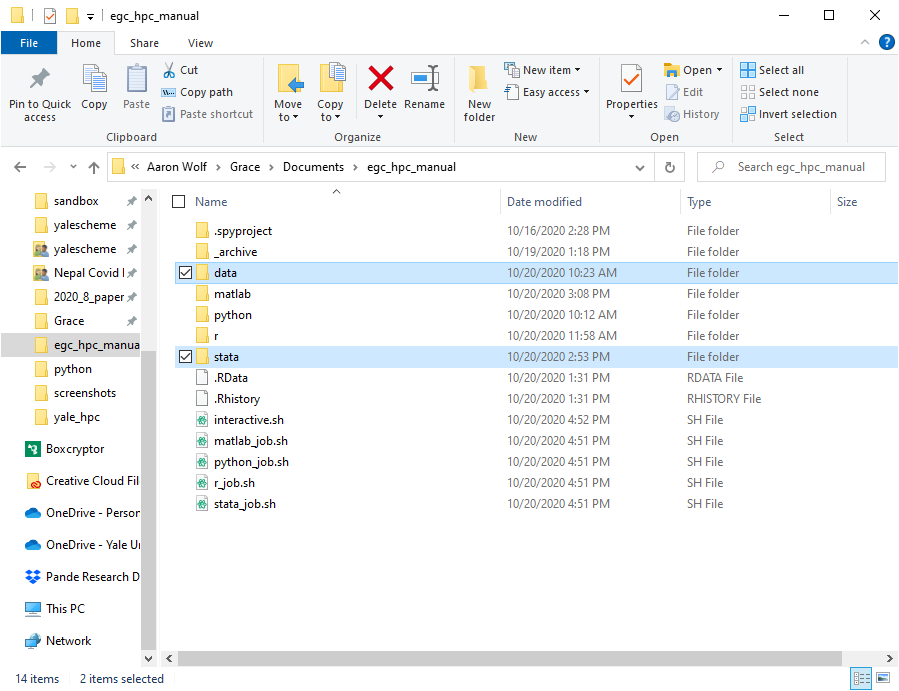
\includegraphics[width=0.7\textwidth]{screenshots/fig9a.PNG} 
\end{frame}

\begin{frame}{Step 2: Create.do file}
\center
Create a master do file, as well as a sub-files (we'll call this one \textit{1\_read.do}, as we will only use it to read in the auto dataset). The following slides will provide the content of these files.
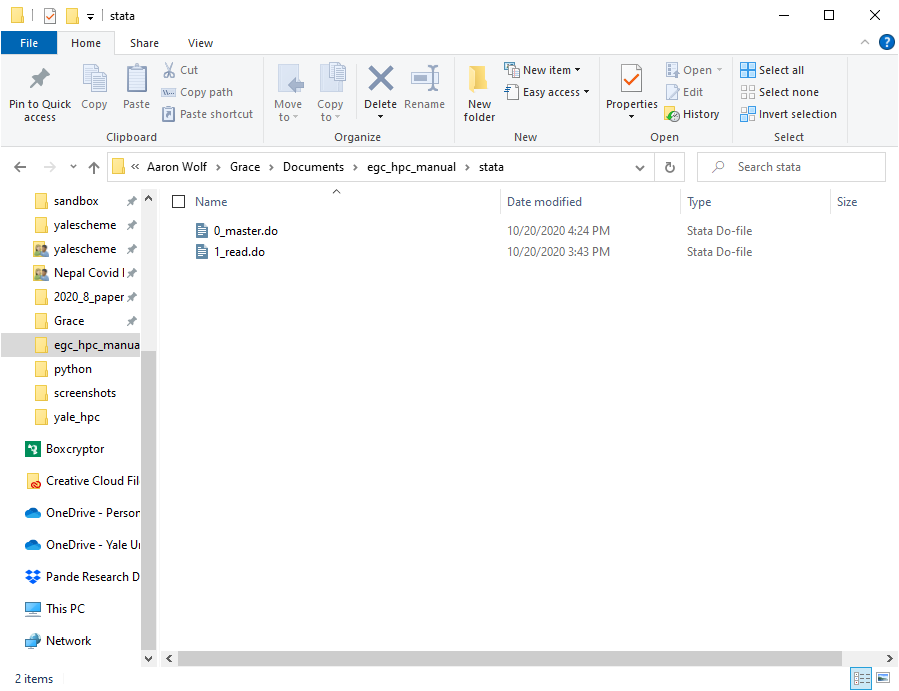
\includegraphics[width=0.8\textwidth]{screenshots/fig9b.PNG} 
\end{frame}


\begin{frame}[fragile]{Step 2: Create.do file - 0\_master.do}
\center
\only<1>{\addtocounter{lstlisting}{0}
\lstinputlisting[linerange={1-13},language=stata,style=stata-editor,caption={0\_master.do},basicstyle=\tiny]{../stata/0_master.do}}
\only<2>{\addtocounter{lstlisting}{-1}
\lstinputlisting[linerange={16-40},language=stata,style=stata-editor,caption={0\_master.do},basicstyle=\tiny]{../stata/0_master.do}}
\end{frame}


\begin{frame}{Step 3: Create sub files}
Now we can make our subfiles. You can put anything you want here as a test. 

For now, we will just load the auto dataset (saved in the data folder).
\end{frame}

\begin{frame}[fragile]{Step 3: Create sub-file 1\_read.do}
\center
\only<1>{\addtocounter{lstlisting}{0}
\lstinputlisting[linerange={1-16},language=stata,style=stata-editor,caption={1\_read.do},basicstyle=\tiny]{../stata/1_read.do}}
\end{frame}

\begin{frame}{Step 4: Create batch script} 
\center
Next we will write a batch script which will run our master do file.

I will place this close in the project root directory, but you can also put it in your default working directory on Grace, as long as you remember where it is when you use \texttt{sbatch} to call it.

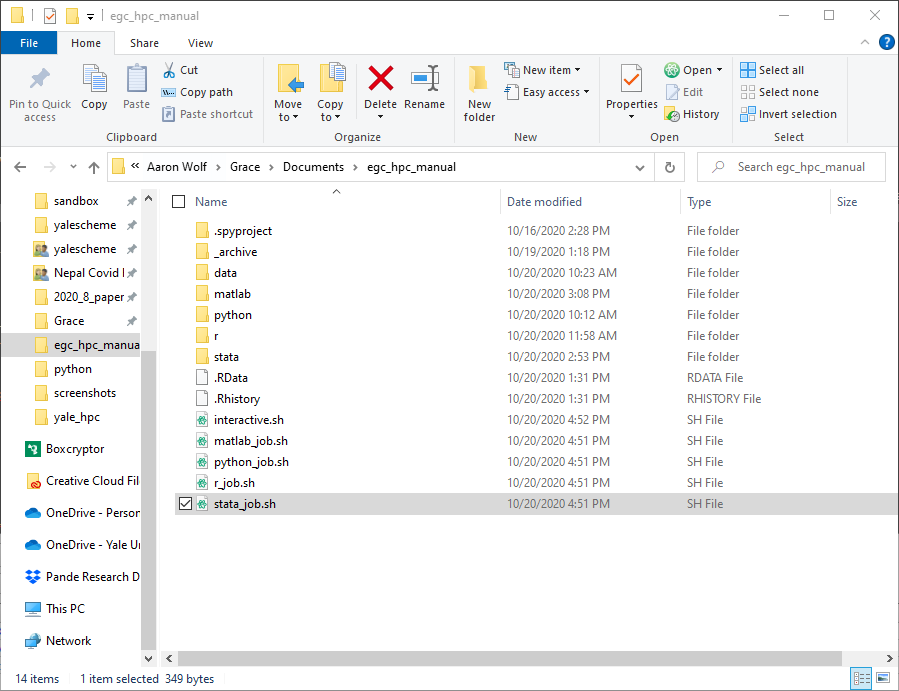
\includegraphics[width=0.7\textwidth]{screenshots/fig10a.PNG} 

\end{frame}


\begin{frame}[fragile]{Step 4: Create batch script - stata\_job.sh}
\center
\lstinputlisting[language=bash,style=bash,caption={stata\_job.sh},basicstyle=\footnotesize]{../stata_job.sh}
\end{frame}

\begin{frame}{Step 6: Synchronize your root folder to your Grace project folder}
\center
\only<1>{Navigate to wherever you want your root directory to exist on Grace in WinSCP and select "Synchronize".}
\only<2>{Choose "Remote" and click "OK".}
\only<3>{Select all files and click "OK".}


\includegraphics<1>[width=0.9\textwidth]{screenshots/fig11a.PNG}
\includegraphics<2>[width=0.6\textwidth]{screenshots/fig11b.PNG}
\includegraphics<3>[width=0.7\textwidth]{screenshots/fig11c.PNG}

\end{frame}

\begin{frame}{Step 7: Run batch file}
\center
\only<1>{Open MobaXterm and input the following code (substituting the path for your .sh file): \\ \texttt{sbatch Documents/egc\_hpc\_manual/stata\_job.sh}}
\only<2>{You should see a message indicating the job was submitted. You can now input the following command (insert your username) to monitor the status of your job requests: \\ \texttt{squeue -u abc123}}
\only<3>{When Grace finishes your file, you will receive an email, and an output file in your home directory with the results (i.e. output screen). This can be used to diagnose errors and ensure everything ran.}


\includegraphics<1>[width=0.7\textwidth]{screenshots/fig11d.PNG}
\includegraphics<2>[width=0.7\textwidth]{screenshots/fig11d.PNG}
\includegraphics<3>[width=0.7\textwidth]{screenshots/fig11e.PNG}

\end{frame}

\begin{frame}{That's it!}
\begin{itemize}
\item When starting out, there are likely to be unforeseen errors/issues.
\item We recommend starting with a similar example project and submitting batch scripts that ask for minimal resources to ensure you get all the paths right.
\item Once the script runs smoothly without errors, switch the .do files called to the real ones and adjust the resource request accordingly.
\end{itemize}
\end{frame}





\section{Python}
\subsection{Getting Started}

\begin{frame}{HPC: but with Python (!)}
\begin{itemize}
\item Python code can be run directly from the command line using the \texttt{python myscrip.py} syntax.
\item However, similar to Stata, where we had to ``load" Stata MP (\texttt{module load Stata/15}), we need to tell Grace to find and use a Python installation.
\item For this, we use an Anaconda Python environment.
\end{itemize}
\end{frame}

\begin{frame}{What's Anaconda?}
\begin{itemize}
\item If you've never used Anaconda think of it this way: Anaconda is to Python (and R!) what the App Store is to Apps. It is a single place to manage your installations of Python and R.
\item Anaconda allows you to set up and control multiple Python ``Environments": Separate installations of Python with different characteristics (e.g. you could have one environment on your computer with Python 2.7, and another with Python 3.6). In each environment, you can install all the packages you usually would with PIP.
\item Anaconda is free for individual use: Check out \href{https://www.anaconda.com/}{https://www.anaconda.com/}.
\item \textbf{Before you can use Python on Grace, you need to first create a Python environment.} You can do this on a login node or an interactive node.
\end{itemize}
\end{frame}

\begin{frame}{Create a new Python Environment called ``py3\_base"}
\center
\only<1>{Open MobaXTerm, login, and start a new interactive session: \\ \texttt{srun --pty -c 4 -p interactive -t 4:00:00 bash}}
\only<2>{Load the \texttt{miniconda} module: \\ \texttt{module load miniconda}}
\only<3>{Create a new Python environment with a few basic data science packages installed by default: \\ \texttt{\tiny conda create -n py3\_base python=3 numpy scipy matplotlib pandas ipython jupyter jupyterlab} }
\only<4>{Now, whenever you want to use Python, whether in an interactive session or batch file, simply load up miniconda, and activate the environment: \\ \texttt{module load miniconda} \\ \texttt{conda activate py3\_base}}
\only<5>{You can even start an ipython session for interactive Python! \\ \texttt{ipython}}
\only<6>{When you're done, deactivate the current environment: \\ \texttt{conda deactivate}}

\includegraphics<1>[width=0.9\textwidth]{screenshots/fig12a.PNG}
\includegraphics<2>[width=0.9\textwidth]{screenshots/fig12b.PNG}
\includegraphics<3>[width=0.9\textwidth]{screenshots/fig12c.PNG}
\includegraphics<4>[width=0.9\textwidth]{screenshots/fig12d.PNG}
\includegraphics<5>[width=0.9\textwidth]{screenshots/fig12e.PNG}
\includegraphics<6>[width=0.9\textwidth]{screenshots/fig12f.PNG}

\end{frame}

\subsection{Example Project}
\begin{frame}[standout]
  Python Example Project
\end{frame}

\begin{frame}{Python Example Project}
Now, let's create a new Python project with a batch script, master .py files, and .py files with the core analysis commands.

We will set it up so that you can run the .py file on your own computer as well as Grace (once the files are synchronized).

Then we will create a batch script that will run the master .py file, which will itself run all the project .py files.
\end{frame}

\begin{frame}{Step 1: Create project folder}
\center
Create a new folder on your PC anywhere you like. This will be your main (root) folder. \\ Add folders for data and python files.
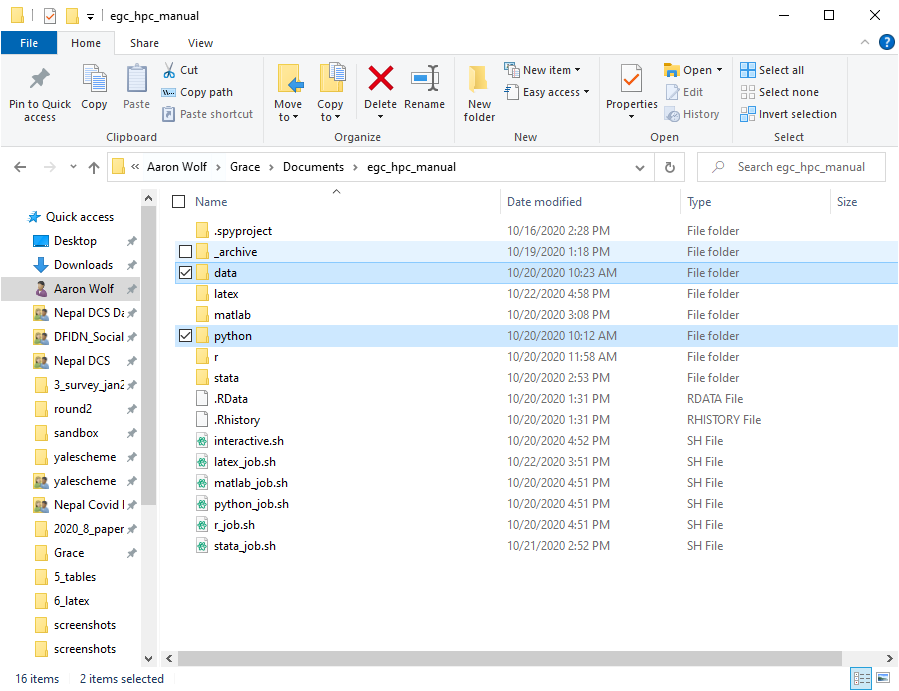
\includegraphics[width=0.7\textwidth]{screenshots/fig13a.PNG} 
\end{frame}

\begin{frame}{Step 2: Create .py files}
\center
Create a master .py file, as well as a sub-files (we'll call this one \textit{1\_read.py}, as we will only use it to read in the auto dataset). The following slides will provide the content of these files.
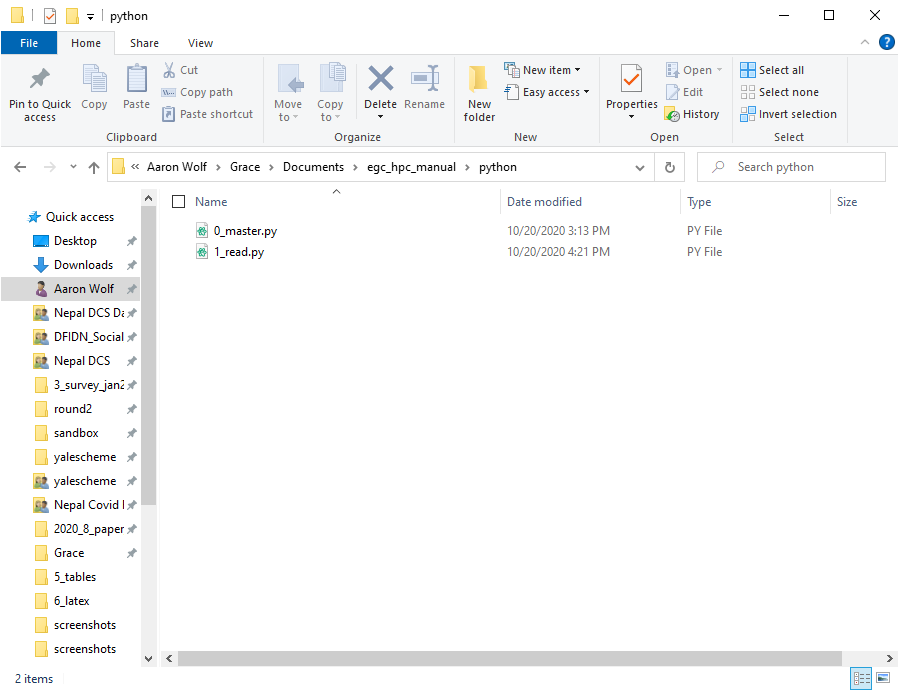
\includegraphics[width=0.8\textwidth]{screenshots/fig13b.PNG} 
\end{frame}


\begin{frame}[fragile]{Step 2: Create .py file - 0\_master.py}
\center
\only<1>{\addtocounter{lstlisting}{0}
\lstinputlisting[linerange={1-13},language=Python,caption={0\_master.py},basicstyle=\tiny]{../python/0_master.py}}
\only<2>{\addtocounter{lstlisting}{-1}
\lstinputlisting[linerange={16-40},language=Python,caption={0\_master.py},basicstyle=\tiny]{../python/0_master.py}}
\end{frame}


\begin{frame}{Step 3: Create sub files}
Now we can make our subfiles. You can put anything you want here as a test. 

For now, we will just load the auto dataset (saved in the data folder).
\end{frame}

\begin{frame}[fragile]{Step 3: Create sub-file 1\_read.py}
\center
\only<1>{\addtocounter{lstlisting}{0}
\lstinputlisting[linerange={1-19},language=Python,caption={1\_read.do},basicstyle=\tiny]{../python/1_read.py}}
\end{frame}

\begin{frame}{Step 4: Create batch script} 
\center
Next we will write a batch script which will run our master .py file.

I will place this close in the project root directory, but you can also put it in your default working directory on Grace, as long as you remember where it is when you use \texttt{sbatch} to call it.

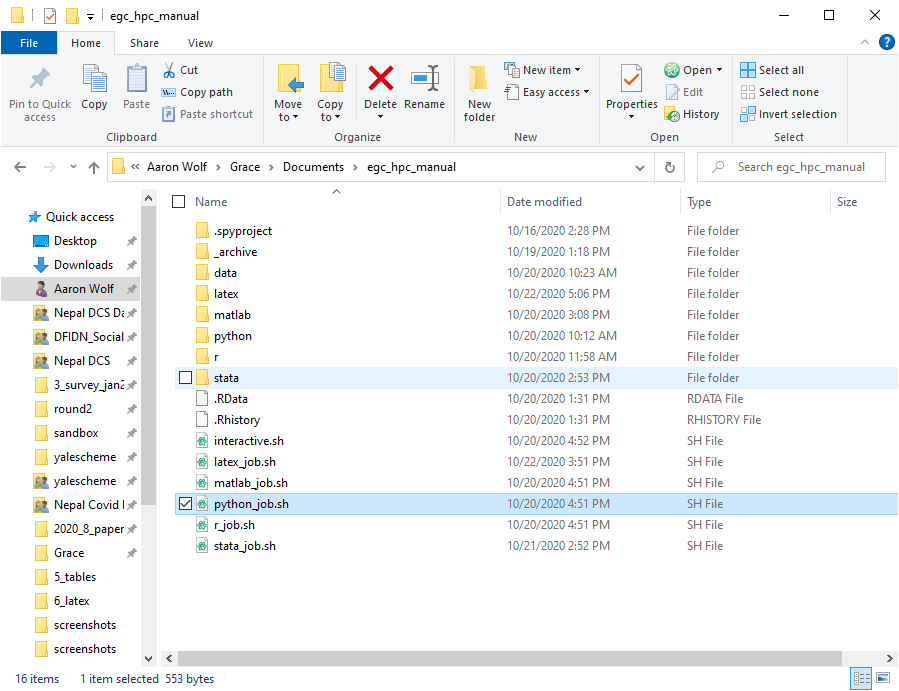
\includegraphics[width=0.7\textwidth]{screenshots/fig13c.PNG} 

\end{frame}


\begin{frame}[fragile]{Step 4: Create batch script - python\_job.sh}
Note: I have included the line to create the new python environment. If you have not already created it, make sure to include this (or create it in a separate interactive session).
\center
\lstinputlisting[language=bash,style=bash,caption={python\_job.sh},basicstyle=\tiny]{../python_job.sh}
\end{frame}

\begin{frame}{Step 6: Synchronize your root folder to your Grace project folder}
\center
\only<1>{Navigate to wherever you want your root directory to exist on Grace in WinSCP and select "Synchronize". Choose your files and click ``OK".}

\includegraphics<1>[width=0.9\textwidth]{screenshots/fig11a.PNG}
\end{frame}

\begin{frame}{Step 7: Run batch file}
\center
\only<1>{Open MobaXterm and input the following code (substituting the path for your .sh file): \\ \texttt{sbatch Documents/egc\_hpc\_manual/python\_job.sh}}
\only<2>{You should see a message indicating the job was submitted. You can now input the following command (insert your username) to monitor the status of your job requests: \\ \texttt{squeue -u abc123}}
\only<3>{When Grace finishes your file, you will receive an email, and an output file in your home directory with the results (i.e. output screen). This can be used to diagnose errors and ensure everything ran.}


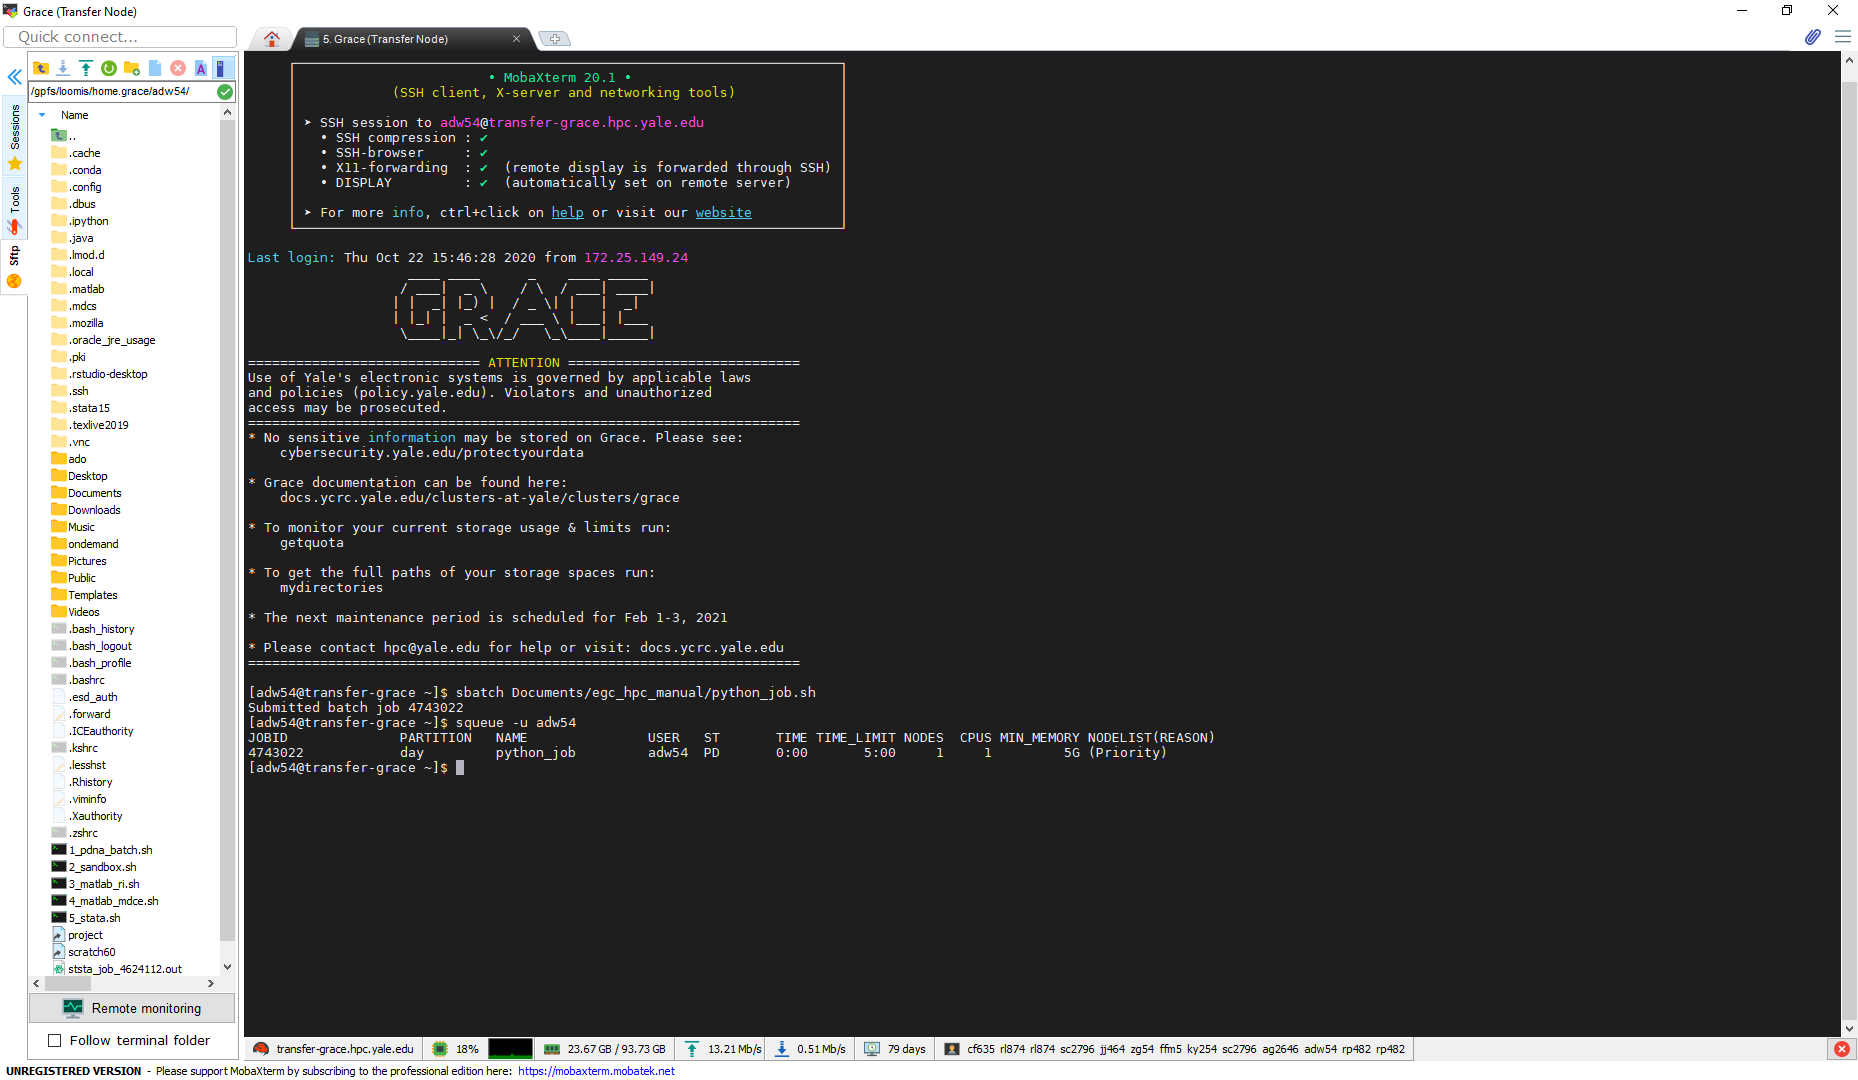
\includegraphics[width=0.9\textwidth]{screenshots/fig13d.PNG}

\end{frame}

\begin{frame}{That's it!}
\begin{itemize}
\item When starting out, there are likely to be unforeseen errors/issues.
\item We recommend starting with a similar example project and submitting batch scripts that ask for minimal resources to ensure you get all the paths right.
\item Once the script runs smoothly without errors, switch the .py files called to the real ones and adjust the resource request accordingly.
\end{itemize}
\end{frame}



\addtocontents{toc}{\newpage}
\section{R}
\subsection{Getting Started}

\begin{frame}{HPC: but with R (!)}
\begin{itemize}
\item R code can be run directly from the command line using the \texttt{R --slave -f myscript.R} syntax.
\item However, similar to Stata, where we had to ``load" Stata MP (\texttt{module load Stata/15}), we need to tell Grace to find and use an R installation.
\item For this, we use an Anaconda R environment.
\end{itemize}
\end{frame}

\begin{frame}{What's Anaconda?}
\begin{itemize}
\item If you've never used Anaconda think of it this way: Anaconda is to Python (and R!) what the App Store is to Apps. It is a single place to manage your installations of Python and R.
\item Anaconda allows you to set up and control multiple R ``Environments": Separate installations of R with different characteristics (e.g. you could have one environment on your computer with r-essentials, and another with specific machine learning libraries installed). In each environment, you can install all the libraries/packages you usually would with \texttt{install.packages}.
\item Anaconda is free for individual use: Check out \href{https://www.anaconda.com/}{https://www.anaconda.com/}.
\item \textbf{Before you can use R on Grace, you need to first create an R environment.} You can do this on a login node or an interactive node.
\end{itemize}
\end{frame}

\begin{frame}{Create a new R Environment called ``r3\_base"}
\center
\only<1>{Open MobaXTerm, login, and start a new interactive session: \\ \texttt{srun --pty -c 4 -p interactive -t 4:00:00 bash}}
\only<2>{Load the \texttt{miniconda} module: \\ \texttt{module load miniconda}}
\only<3>{Create a new R environment with a few basic data science packages installed by default: \\ \texttt{\tiny conda create --name r3\_base r-base r-essentials r-doMC r-Rmpi} }
\only<4>{Now, whenever you want to use R, whether in an interactive session or batch file, simply load up miniconda, and activate the environment: \\ \texttt{module load miniconda} \\ \texttt{conda activate r3\_base}}
\only<5>{You can even start an R session for interactive R! \\ \texttt{R}}
\only<6>{When you're done, deactivate the current environment: \\ \texttt{conda deactivate}}

\includegraphics<1>[width=0.9\textwidth]{screenshots/fig16a.PNG}
\includegraphics<2>[width=0.9\textwidth]{screenshots/fig16b.PNG}
\includegraphics<3>[width=0.9\textwidth]{screenshots/fig16c.PNG}
\includegraphics<4>[width=0.9\textwidth]{screenshots/fig16d.PNG}
\includegraphics<5>[width=0.9\textwidth]{screenshots/fig16e.PNG}
\includegraphics<6>[width=0.9\textwidth]{screenshots/fig16f.PNG}

\end{frame}

\subsection{Example Project}
\begin{frame}[standout]
  R Example Project
\end{frame}

\begin{frame}{R Example Project}
Now, let's create a new R project with a batch script, master .R files, and .R files with the core analysis commands.

We will set it up so that you can run the .R file on your own computer as well as Grace (once the files are synchronized).

Then we will create a batch script that will run the master .R file, which will itself run all the project .R files.
\end{frame}

\begin{frame}{Step 1: Create project folder}
\center
Create a new folder on your PC anywhere you like. This will be your main (root) folder. \\ Add folders for data and R files.
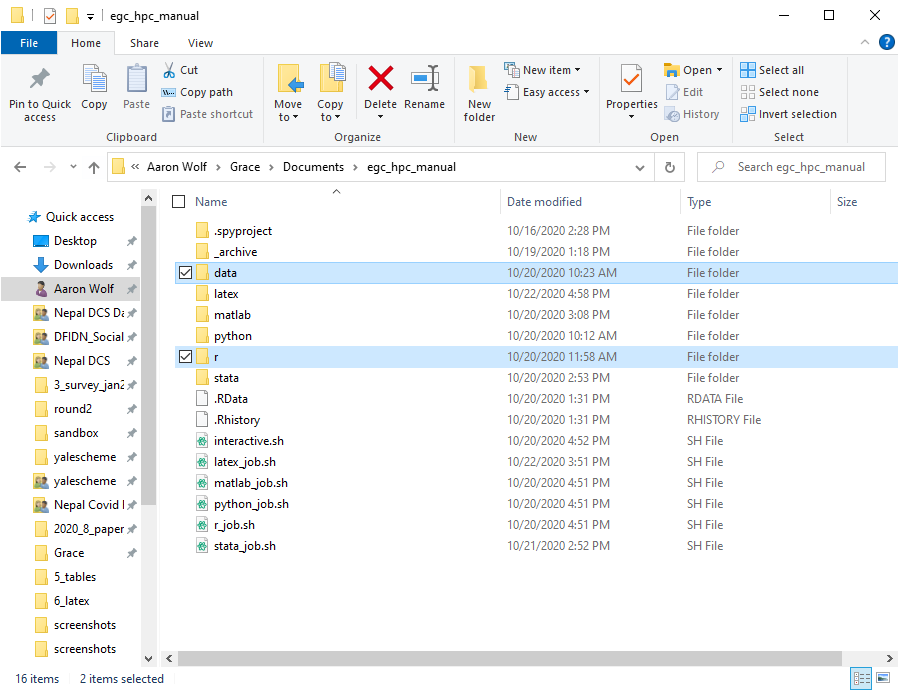
\includegraphics[width=0.7\textwidth]{screenshots/fig14a.PNG} 
\end{frame}

\begin{frame}{Step 2: Create .R files}
\center
Create a master .R file, as well as a sub-files (we'll call this one \textit{1\_read.R}, as we will only use it to read in the auto dataset). The following slides will provide the content of these files.
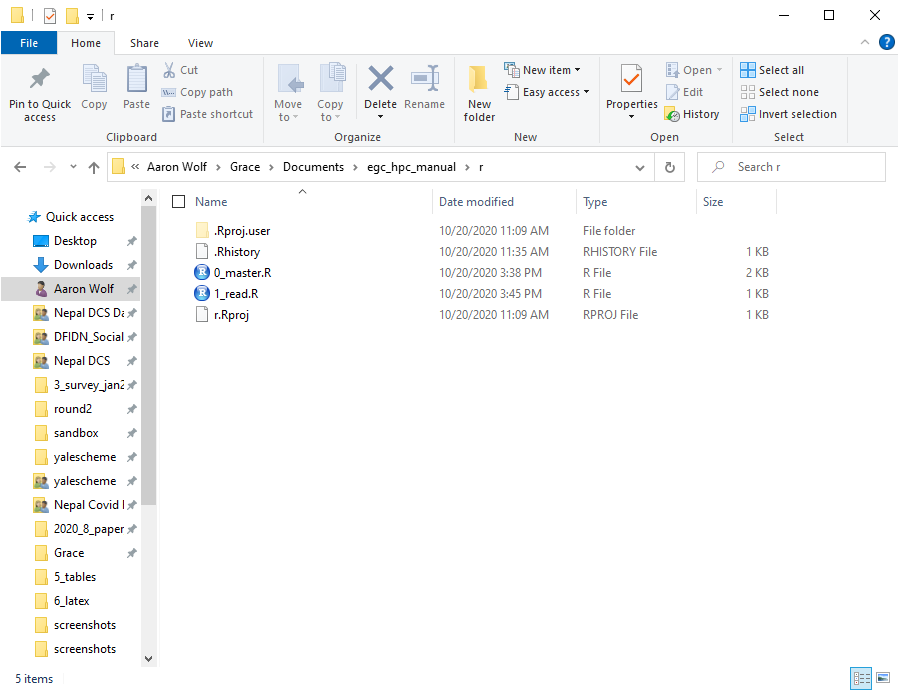
\includegraphics[width=0.8\textwidth]{screenshots/fig14b.PNG} 
\end{frame}


\begin{frame}[fragile]{Step 2: Create .R file - 0\_master.R}
\center
\only<1>{\addtocounter{lstlisting}{0}
\lstinputlisting[linerange={1-13},language=R,caption={0\_master.R},basicstyle=\tiny]{../r/0_master.R}}
\only<2>{\addtocounter{lstlisting}{-1}
\lstinputlisting[linerange={16-40},language=R,caption={0\_master.R},basicstyle=\tiny]{../r/0_master.R}}
\end{frame}


\begin{frame}{Step 3: Create sub files}
Now we can make our subfiles. You can put anything you want here as a test. 

For now, we will just load the auto dataset (saved in the data folder).
\end{frame}

\begin{frame}[fragile]{Step 3: Create sub-file 1\_read.R}
\center
\only<1>{\addtocounter{lstlisting}{0}
\lstinputlisting[linerange={1-19},language=Python,caption={1\_read.do},basicstyle=\tiny]{../r/1_read.R}}
\end{frame}

\begin{frame}{Step 4: Create batch script} 
\center
Next we will write a batch script which will run our master .R file.

I will place this close in the project root directory, but you can also put it in your default working directory on Grace, as long as you remember where it is when you use \texttt{sbatch} to call it.

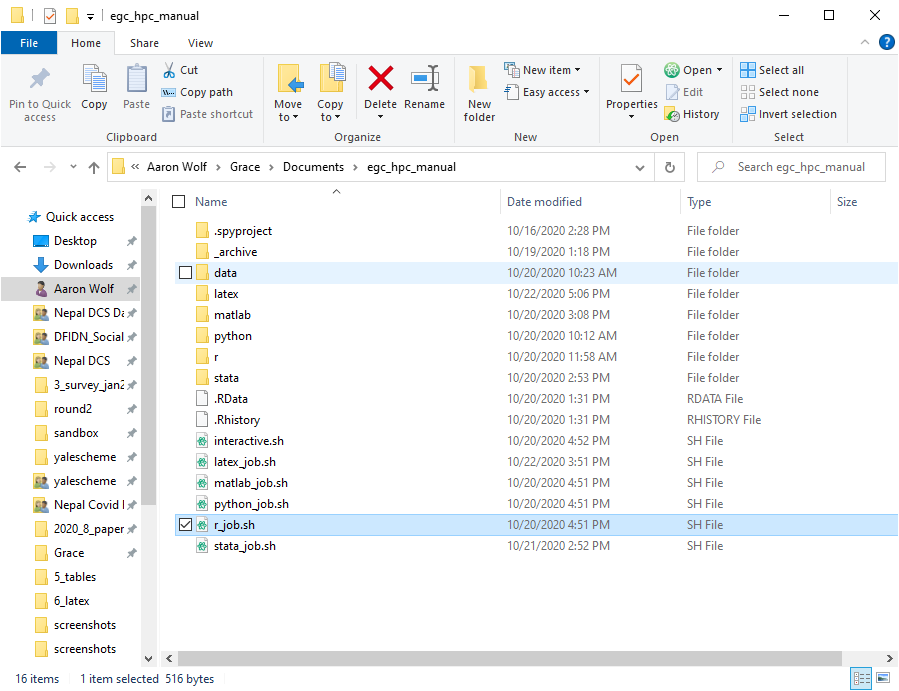
\includegraphics[width=0.7\textwidth]{screenshots/fig14c.PNG} 

\end{frame}


\begin{frame}[fragile]{Step 4: Create batch script - r\_job.sh}
Note: I have included the line to create the new R environment. If you have not already created it, make sure to include this (or create it in a separate interactive session).
\center
\lstinputlisting[language=bash,style=bash,caption={r\_job.sh},basicstyle=\tiny]{../r_job.sh}
\end{frame}

\begin{frame}{Step 6: Synchronize your root folder to your Grace project folder}
\center
\only<1>{Navigate to wherever you want your root directory to exist on Grace in WinSCP and select "Synchronize". Choose your files and click ``OK".}

\includegraphics<1>[width=0.9\textwidth]{screenshots/fig11a.PNG}
\end{frame}

\begin{frame}{Step 7: Run batch file}
\center
\only<1>{Open MobaXterm and input the following code (substituting the path for your .sh file): \\ \texttt{sbatch Documents/egc\_hpc\_manual/r\_job.sh}}
\only<2>{You should see a message indicating the job was submitted. You can now input the following command (insert your username) to monitor the status of your job requests: \\ \texttt{squeue -u abc123}}
\only<3>{When Grace finishes your file, you will receive an email, and an output file in your home directory with the results (i.e. output screen). This can be used to diagnose errors and ensure everything ran.}


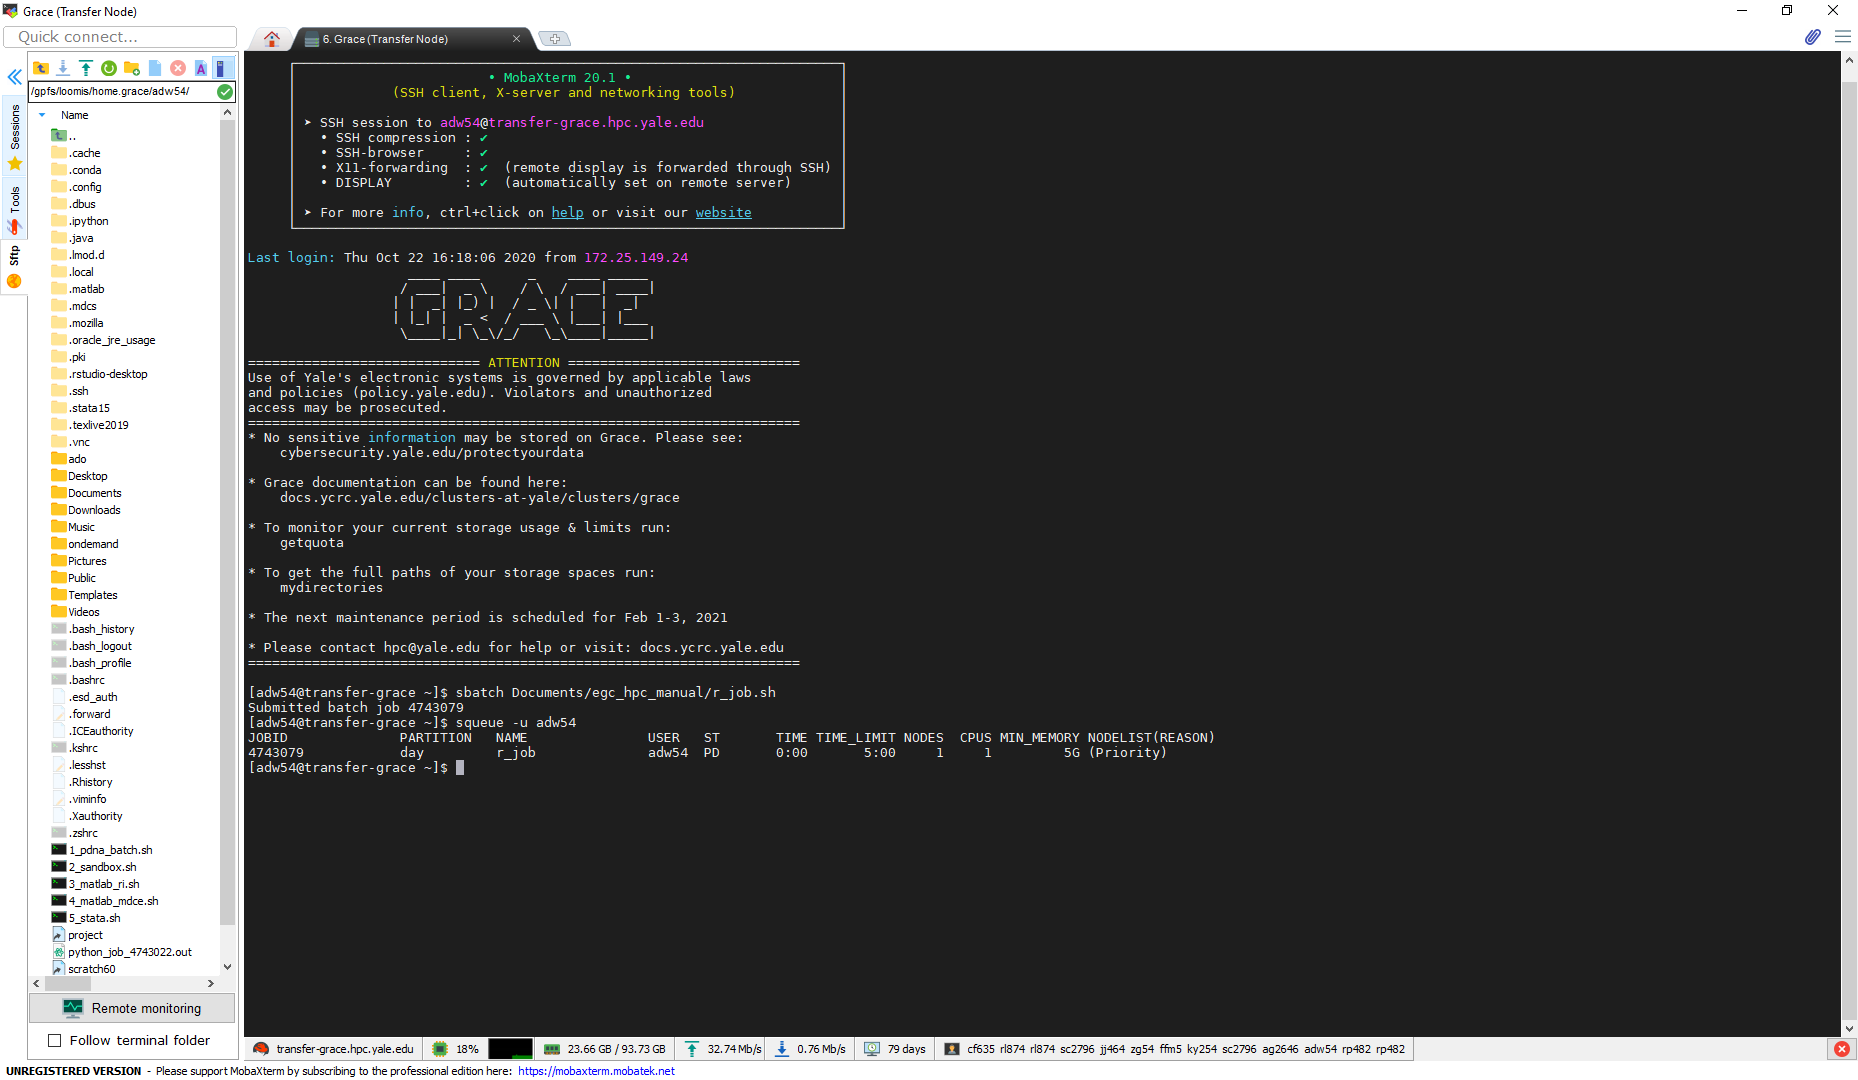
\includegraphics[width=0.9\textwidth]{screenshots/fig14d.PNG}

\end{frame}

\begin{frame}{That's it!}
\begin{itemize}
\item When starting out, there are likely to be unforeseen errors/issues.
\item We recommend starting with a similar example project and submitting batch scripts that ask for minimal resources to ensure you get all the paths right.
\item Once the script runs smoothly without errors, switch the .R files called to the real ones and adjust the resource request accordingly.
\end{itemize}
\end{frame}





\section{Matlab}
\subsection{Getting Started}

\begin{frame}{HPC: but with Matlab (!)}
\begin{itemize}
\item Matlab code can be run directly from the command line using the \texttt{matlab} command (for interactive matlab) or \texttt{matlab -nodisplay < myscript.m} (to run a specific file).
\item However, similar to Stata, where we had to ``load" Stata MP (\texttt{module load Stata/15}), we need to tell Grace to find and use a matlab installation.
\item For this, we simply type in \texttt{module load MATLAB/2020a}.
\item There are actually multiple flavors of Matlab available. You'll likely want to stick with the latest, but if you need to use Matlab parallel, you can use \texttt{module load MATLAB/2019a-parallel}.
\item Check out all available versions of Matlab using \texttt{module spider Matlab}
\item Let's try running Matlab from the command line in Grace...
\end{itemize}
\end{frame}

\begin{frame}
\center
\only<1>{Open MobaXTerm, login, and start a new interactive session: \\ \texttt{srun --pty -c 4 -p interactive -t 4:00:00 bash}}
\only<2>{Load the \texttt{miniconda} module: \\ \texttt{module load MATLAB/2019a-parallel}}
\only<3>{Run \texttt{matlab} and fiddle around! \\ \texttt{matlab} \\ \texttt{pwd}}

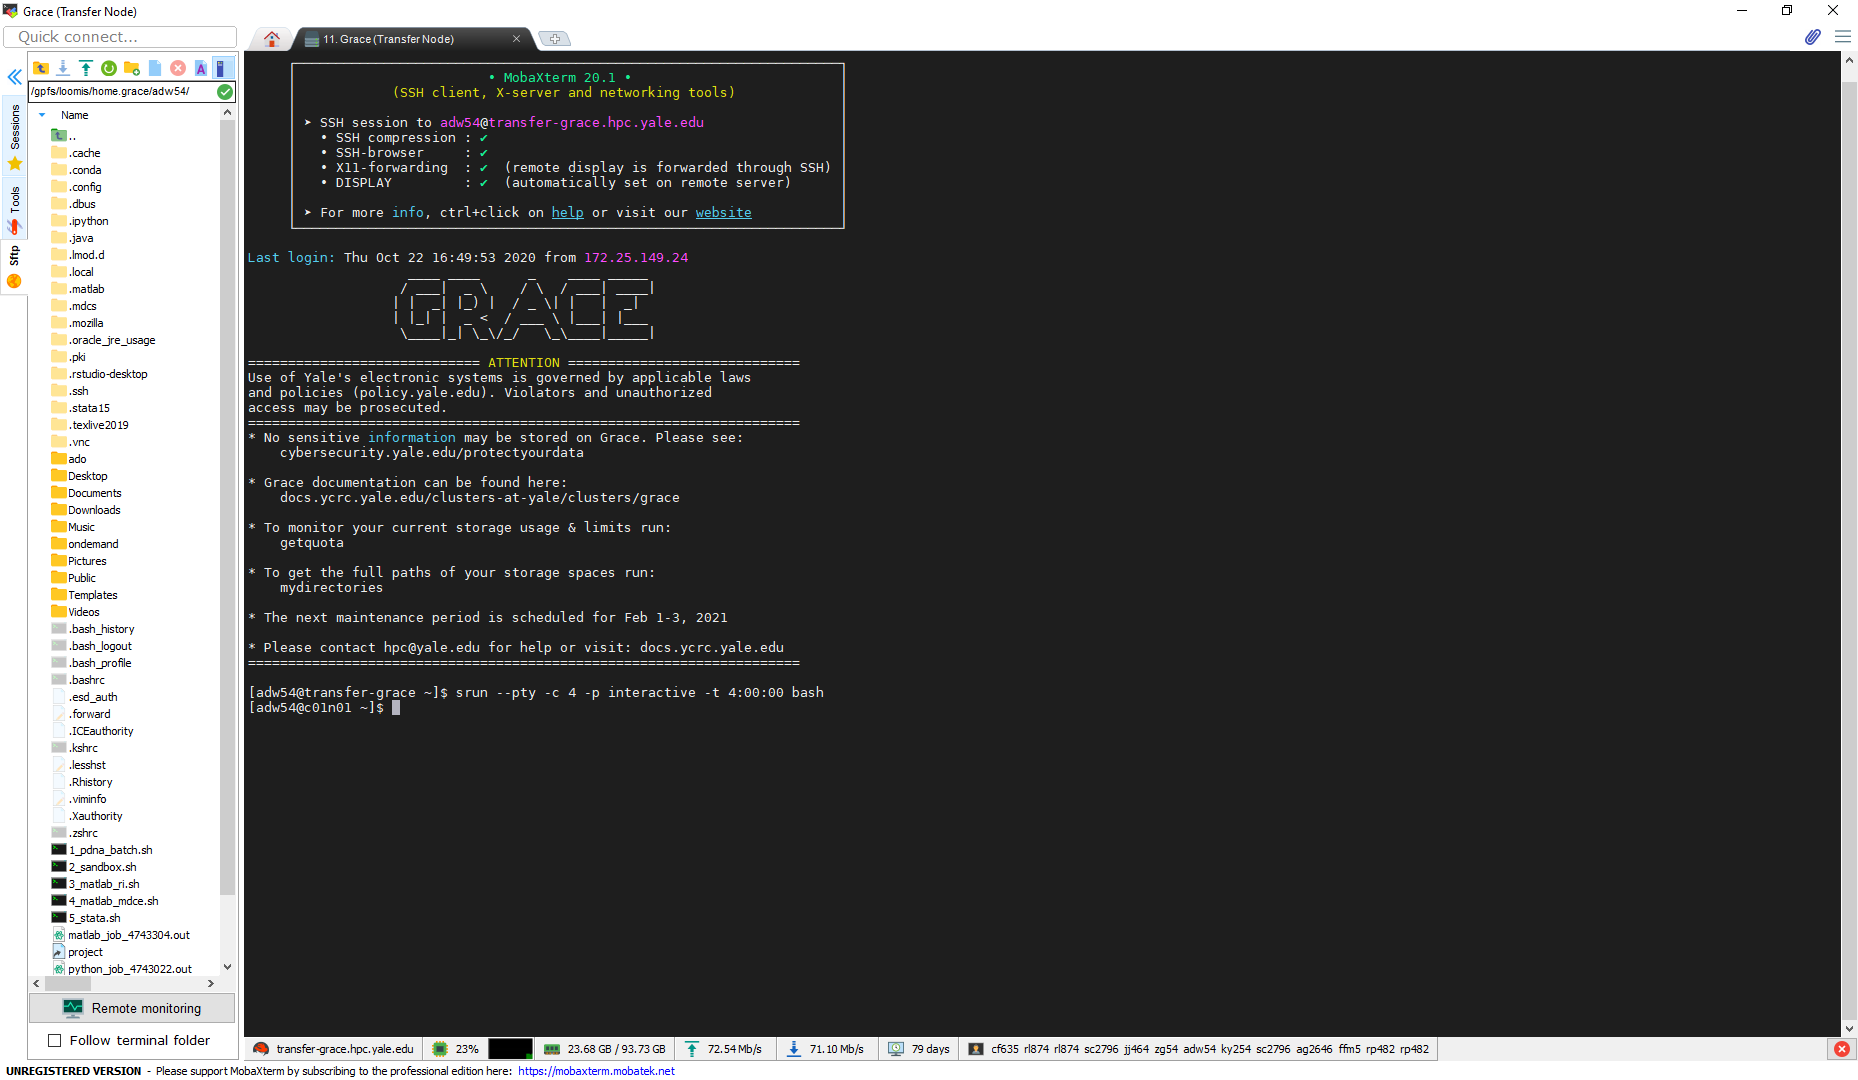
\includegraphics[width=0.9\textwidth]{screenshots/fig17a.PNG}
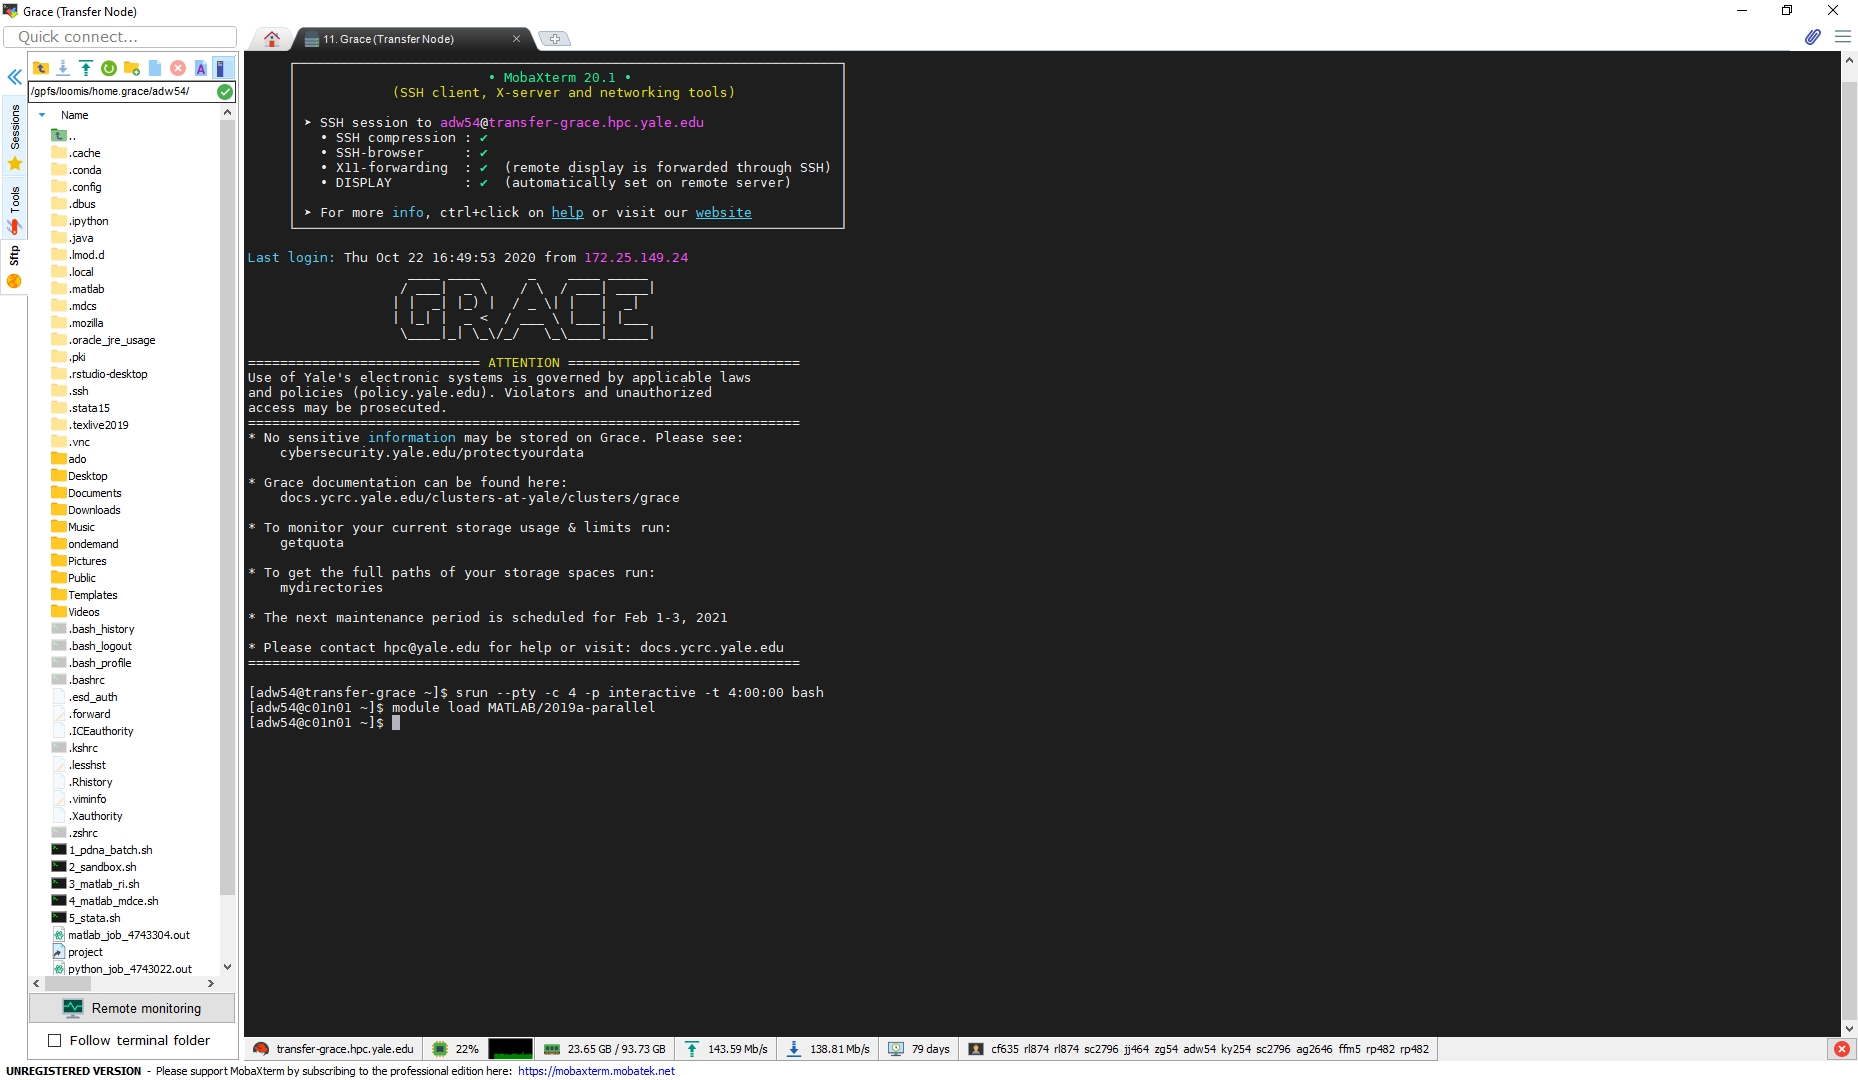
\includegraphics[width=0.9\textwidth]{screenshots/fig17b.PNG}
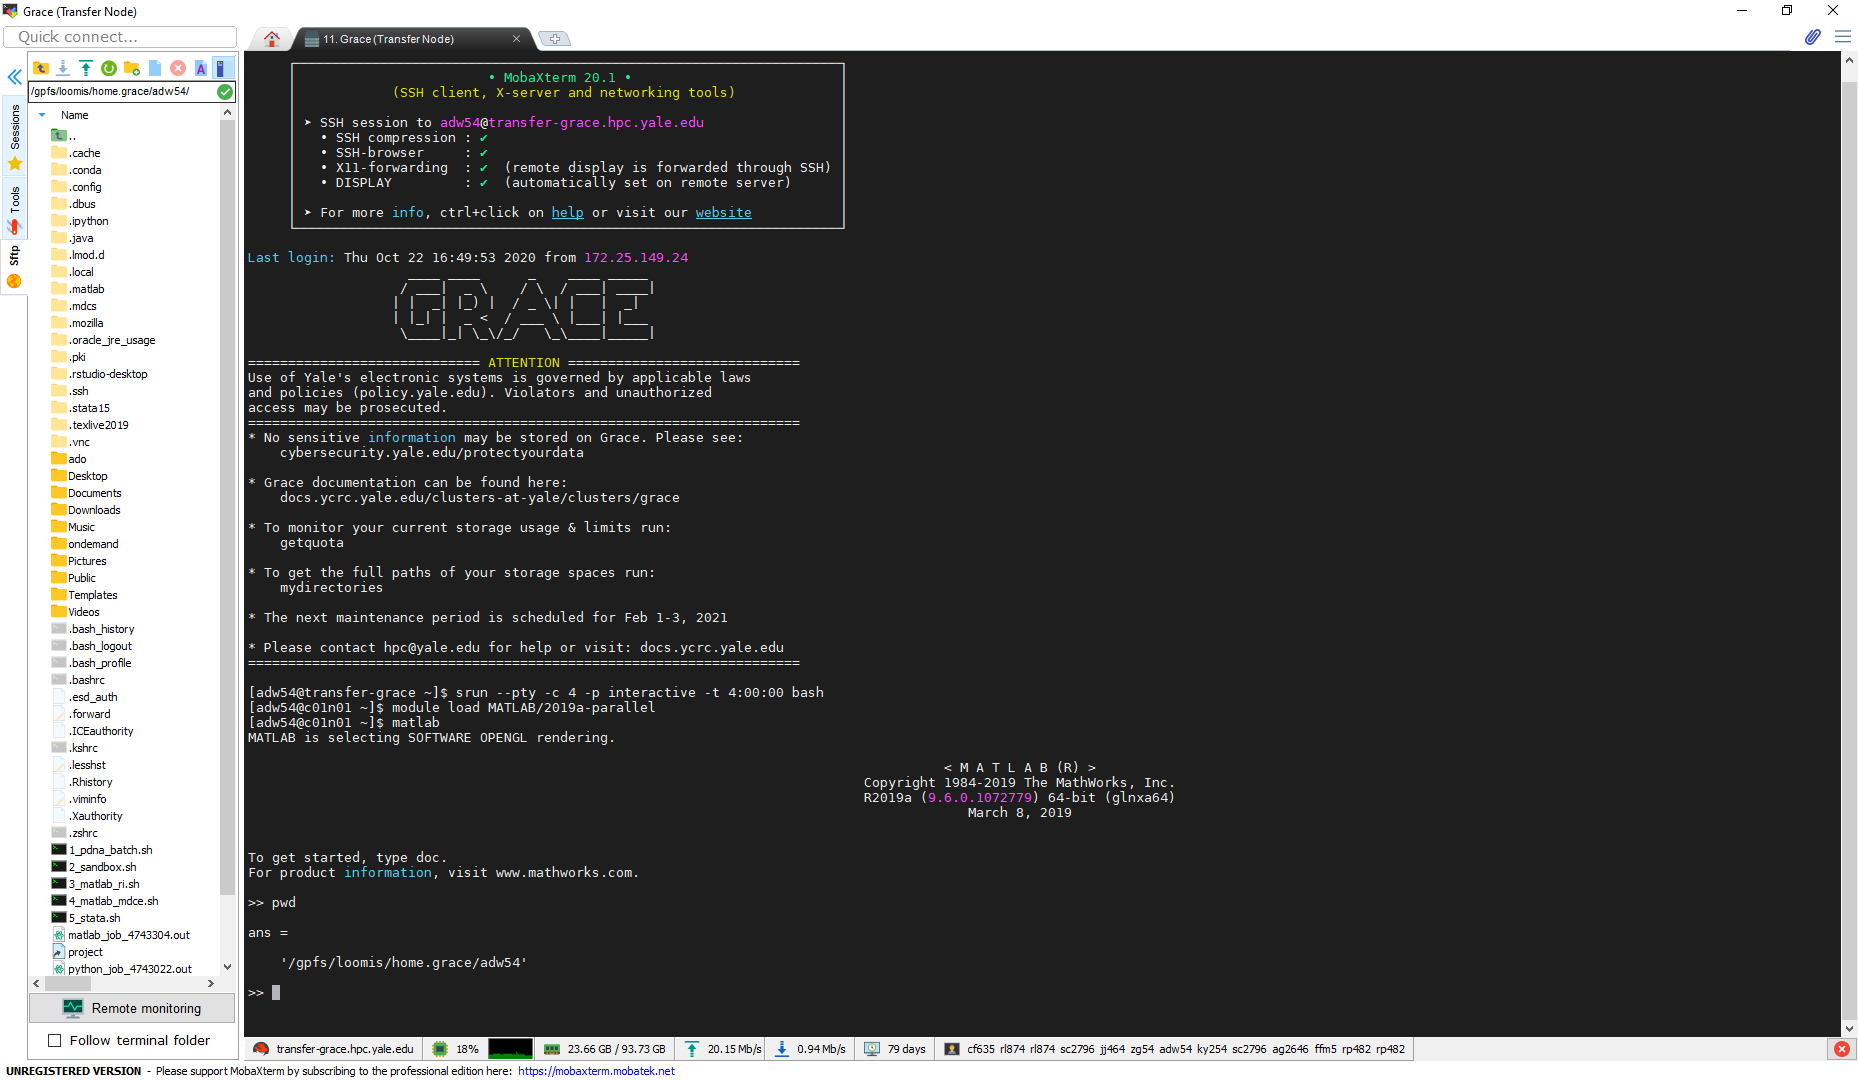
\includegraphics[width=0.9\textwidth]{screenshots/fig17c.PNG}

\end{frame}



\subsection{Example Project}
\begin{frame}[standout]
  Matlab Example Project
\end{frame}

\begin{frame}{Matlab Example Project}
Now, let's create a new R project with a batch script, master .R files, and .R files with the core analysis commands.

We will set it up so that you can run the .R file on your own computer as well as Grace (once the files are synchronized).

Then we will create a batch script that will run the master .R file, which will itself run all the project .R files.
\end{frame}

\begin{frame}{Step 1: Create project folder}
\center
Create a new folder on your PC anywhere you like. This will be your main (root) folder. \\ Add folders for data and .m files.
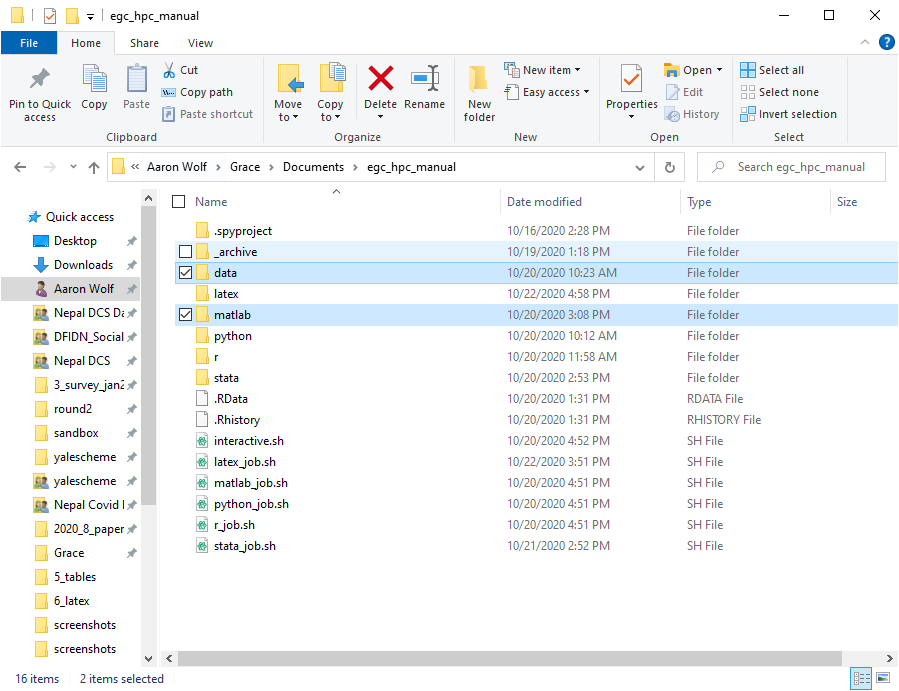
\includegraphics[width=0.7\textwidth]{screenshots/fig15a.PNG} 
\end{frame}

\begin{frame}{Step 2: Create .m files}
\center
Create a master .m file, as well as a sub-files (we'll call this one \textit{read.m}, as we will only use it to read in the auto dataset). The following slides will provide the content of these files.
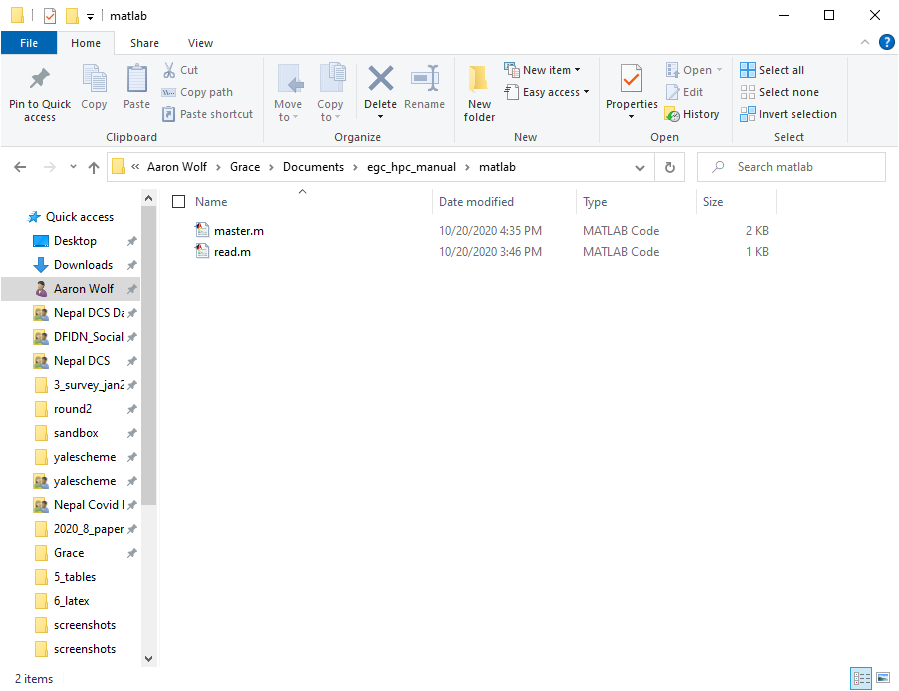
\includegraphics[width=0.8\textwidth]{screenshots/fig15b.PNG} 
\end{frame}


\begin{frame}[fragile]{Step 2: Create .m file - master.m}
\center
\only<1>{\addtocounter{lstlisting}{0}
\lstinputlisting[linerange={1-13},style=Matlab-editor,caption={master.m},basicstyle=\tiny]{../matlab/master.m}}
\only<2>{\addtocounter{lstlisting}{-1}
\lstinputlisting[linerange={16-40},style=Matlab-editor,caption={0\_master.R},basicstyle=\tiny]{../matlab/master.m}}
\end{frame}


\begin{frame}{Step 3: Create sub files}
Now we can make our subfiles. You can put anything you want here as a test. 

For now, we will just load the auto dataset (saved in the data folder).
\end{frame}

\begin{frame}[fragile]{Step 3: Create sub-file read.m}
\center
\only<1>{\addtocounter{lstlisting}{0}
\lstinputlisting[linerange={1-19},style=Matlab-editor,caption={read.m},basicstyle=\tiny]{../matlab/read.m}}
\end{frame}

\begin{frame}{Step 4: Create batch script} 
\center
Next we will write a batch script which will run our master .m file.

I will place this close in the project root directory, but you can also put it in your default working directory on Grace, as long as you remember where it is when you use \texttt{sbatch} to call it.

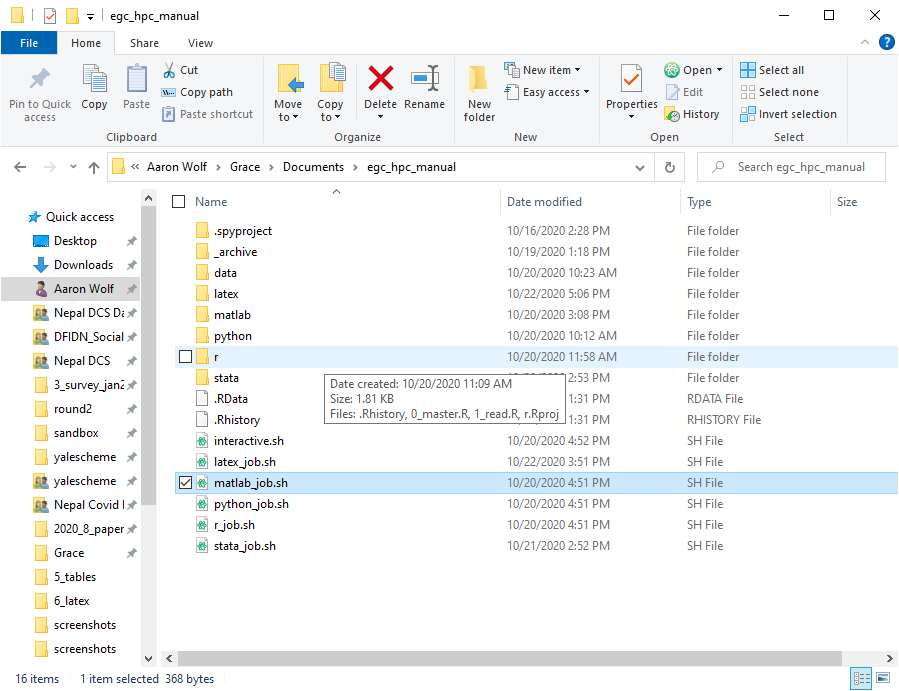
\includegraphics[width=0.7\textwidth]{screenshots/fig15c.PNG} 

\end{frame}


\begin{frame}[fragile]{Step 4: Create batch script - matlab\_job.sh}
\center
\lstinputlisting[language=bash,style=bash,caption={matlab\_job.sh},basicstyle=\footnotesize]{../matlab_job.sh}
\end{frame}

\begin{frame}{Step 6: Synchronize your root folder to your Grace project folder}
\center
\only<1>{Navigate to wherever you want your root directory to exist on Grace in WinSCP and select "Synchronize". Choose your files and click ``OK".}

\includegraphics<1>[width=0.9\textwidth]{screenshots/fig11a.PNG}
\end{frame}

\begin{frame}{Step 7: Run batch file}
\center
\only<1>{Open MobaXterm and input the following code (substituting the path for your .sh file): \\ \texttt{sbatch Documents/egc\_hpc\_manual/matlab\_job.sh}}
\only<2>{You should see a message indicating the job was submitted. You can now input the following command (insert your username) to monitor the status of your job requests: \\ \texttt{squeue -u abc123}}
\only<3>{When Grace finishes your file, you will receive an email, and an output file in your home directory with the results (i.e. output screen). This can be used to diagnose errors and ensure everything ran.}


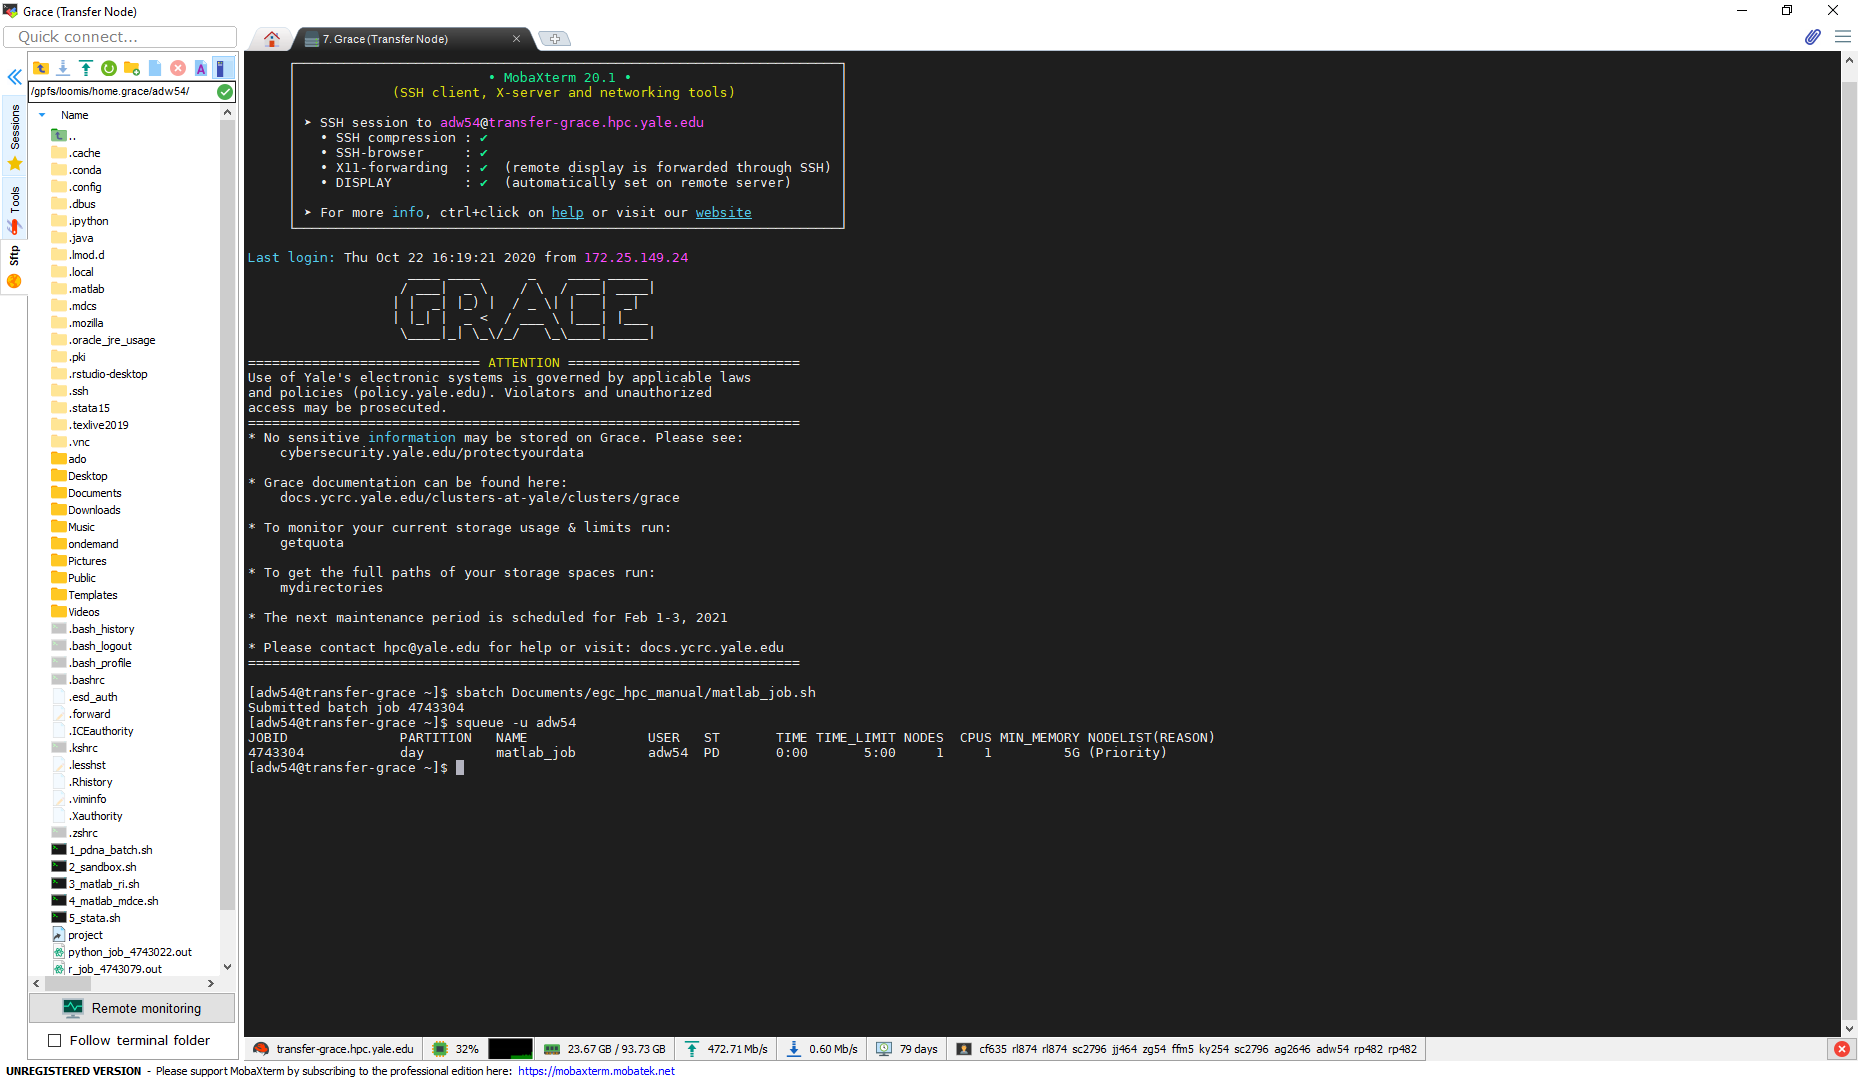
\includegraphics[width=0.9\textwidth]{screenshots/fig15d.PNG}

\end{frame}

\begin{frame}{That's it!}
\begin{itemize}
\item When starting out, there are likely to be unforeseen errors/issues.
\item We recommend starting with a similar example project and submitting batch scripts that ask for minimal resources to ensure you get all the paths right.
\item Once the script runs smoothly without errors, switch the .m files called to the real ones and adjust the resource request accordingly.
\end{itemize}
\end{frame}




\section{\LaTeX}
\begin{frame}{Yup. \LaTeX}
\begin{itemize}
\item You can use \LaTeX~ on Grace to compile your documents!
\item Grace has TeXLive available, and you can use the usual \LaTeX~ commands.
\item Since \LaTeX~ documents are finicky, lets start by simply compiling the base sample2e.tex document.
\end{itemize}
\end{frame}

\begin{frame}{Load \LaTeX~ and compile sample2e document}
\center
\only<1>{Open MobaXTerm, login, and start a new interactive session: \\ \texttt{srun --pty -c 4 -p interactive -t 4:00:00 bash}}
\only<2>{Load the \texttt{TeXLive} module: \\ \texttt{module load TeXLive/2019}}
\only<3>{CD to the directory where your \LaTeX~ document is located, or where you want the sample2e document saved. \\ \texttt{cd Documents/egc\_hpc\_manual/latex}}
\only<4>{Compile your document \\ \texttt{pdflatex sample2e.tex}}
\only<5>{When the document is finished compiling you will see it in the directory you specified.}

\includegraphics<1>[width=0.9\textwidth]{screenshots/fig18a.PNG}
\includegraphics<2>[width=0.9\textwidth]{screenshots/fig18b.PNG}
\includegraphics<3>[width=0.9\textwidth]{screenshots/fig18c.PNG}
\includegraphics<4>[width=0.9\textwidth]{screenshots/fig18d.PNG}
\includegraphics<5>[width=0.9\textwidth]{screenshots/fig18e.PNG}

\end{frame}

\begin{frame}[fragile]{Create a \LaTeX~ batch script - latex\_job.sh}
\center
\lstinputlisting[language=bash,style=bash,caption={latex\_job.sh},basicstyle=\footnotesize]{../latex_job.sh}
\end{frame}


\section{Zoo (Undergrads/CS Students)}

\begin{frame}{Zoo vs HPC?}
\begin{itemize}
\item For undergrads, there are two options in terms of setting up! (a) HPC Grace and (b) the zoo
\item If you already have a zoo account, which you should if you've taken at least one CS class at Yale, using the Zoo will require less setup time
\item Essentially, the following few slides will walk through how to set up the zoo virtual environment and use tmux!
\end{itemize}
\end{frame}

\begin{frame}[fragile]{Zoo: Setup Commands}
After logging into your zoo account, create/go to your dedicated ECG folder and set up a virtual environment: \newline
  
\begin{lstlisting}[language=bash,style=bash]
python -m venv venv 
source venv/bin/activate
pip install selenium bs4 lxml webdrivermanager pandas
\end{lstlisting}

This virtual environment is necessary so you can install the dependencies. Webdrivermanager allows you to use drivers (chromedriver, geckodriver) without needing to wget them! 
\end{frame}

\begin{frame}[fragile]{Zoo: Tmux Commands}
Tmux can be used so you can run multiple jobs within the Zoo. \newline
The commands below detail how to use tmux; do so within the virtual environment. Once in tmux, run job normally then ctrl b, then d to exit. This is the Yale guide: https://docs.ycrc.yale.edu/clusters-at-yale/guides/tmux/ but the two commands below are effectively what you'll need!\newline

\begin{lstlisting}[language=bash,style=bash]
tmux new -s selDemo 
tmux attach -t selDemo

\end{lstlisting}

\end{frame}

\begin{frame}[fragile]{Using Selenium within a Zoo Virtual Env}
Pro tip: you need to specify some initial options for your driver when within a virtual environment. Not all of these are absolutely necessary, but these are the one's I'd recommend:  \newline
\end{frame}

\begin{frame}[fragile]{Using Selenium within a Zoo Virtual Env}
\footnotesize
\begin{lstlisting}[language=python]
chromeOptions = webdriver.ChromeOptions()
chromeOptions.add\textunderscore argument("start-maximized")
chromeOptions.add\textunderscore argument("enable-automation")
chromeOptions.add\textunderscore argument("--headless")
chromeOptions.add\textunderscore argument("--no-sandbox")
chromeOptions.add\textunderscore argument("--disable-infobars")
chromeOptions.add\textunderscore argument("--disable-dev-shm-usage")
chromeOptions.add\textunderscore argument("--disable-browser-side-navigation")
chromeOptions.add\textunderscore argument("--disable-gpu")
driver = webdriver.Chrome(executable\textunderscore path=ChromeDriverManager().install(), options=chromeOptions)
driver.get("insert url")
\end{lstlisting}
\end{frame}


\addtocontents{toc}{\newpage}
\section{Quick Start Guides}
\begin{frame}{Quick Start Guides}
Each of the following slides provides a quick set of commands for those who are familiar with Grace, but need a refresher on the exact commands to run.

\end{frame}


\subsection{Interactive Sessions}
\begin{frame}{Interactive Sessions}
\begin{itemize}
\item Request an interactive session: \\ \alert{\texttt{ srun --pty -c 4 -p interactive -t 4:00:00 bash}}
\item Request an interactive session with X11 (GUI) forwarding: \\ \alert{\texttt{ srun --pty -x11 -c 4 -p interactive -t 4:00:00 bash}}
\end{itemize}
\end{frame}

\subsection{Batch Scripts}
\begin{frame}{Batch Scripts}
\begin{itemize}
\item Run a batch script from the terminal:  \\ \alert{\texttt{ sbatch your\_batch\_script.sh}}
\item Monitor job status: \\ \alert{\texttt{ squeue -u abc123}}
\end{itemize}
\end{frame}

\begin{frame}[fragile]{Batch Scripts}
\lstinputlisting[language=bash,style=bash,caption={stata\_job.sh},basicstyle=\footnotesize]{../stata_job.sh}
\end{frame}


\subsection{Stata}
\begin{frame}{Stata: Interactive}
\alert{\texttt{srun --pty -x11 -c 4 -p interactive -t 4:00:00 bash}}, then \\ 
\alert{\texttt{module load Stata/15}},  followed by  \\ 
\alert{\texttt{stata-mp}} (command-line) or \\ \alert{\texttt{xtata-mp}} (GUI)
\end{frame}

\begin{frame}{Stata: Batch}
\lstinputlisting[language=bash,style=bash,caption={stata\_job.sh},basicstyle=\footnotesize]{../stata_job.sh}
\end{frame}

\subsection{Python}
\begin{frame}{Python: Interactive}
\alert{\texttt{srun --pty -x11 -c 4 -p interactive -t 4:00:00 bash}}, then \\ 
\alert{\texttt{module load miniconda}},  followed by  \\ 
\alert{\texttt{conda create -n py3\_base}} (if not already done), then
\alert{\texttt{conda activate py3\_base}}, then \\
\alert{\texttt{ipython}}
\end{frame}

\begin{frame}{Python: Batch}
\lstinputlisting[language=bash,style=bash,caption={python\_job.sh},basicstyle=\tiny]{../python_job.sh}
\end{frame}

\subsection{R}
\begin{frame}{R: Interactive}
\alert{\texttt{srun --pty -x11 -c 4 -p interactive -t 4:00:00 bash}}, then \\ 
\alert{\texttt{module load miniconda}},  followed by  \\ 
\alert{\texttt{conda create -n r3\_base}} (if not already done), then
\alert{\texttt{conda activate r3\_base}}, then \\
\alert{\texttt{R}}
\end{frame}

\begin{frame}{R: Batch}
\lstinputlisting[language=bash,style=bash,caption={r\_job.sh},basicstyle=\tiny]{../r_job.sh}
\end{frame}

\subsection{Matlab}
\begin{frame}{Matlab: Interactive}
\alert{\texttt{srun --pty -x11 -c 4 -p interactive -t 4:00:00 bash}}, then \\ 
\alert{\texttt{module load MATLAB/2019a-parallel}}, then \\
\alert{\texttt{matlab}}
\end{frame}

\begin{frame}{Matlab: Batch}
\lstinputlisting[language=bash,style=bash,caption={matlab\_job.sh},basicstyle=\footnotesize]{../matlab_job.sh}
\end{frame}

\subsection{\LaTeX}
\begin{frame}{\LaTeX: Interactive}
\alert{\texttt{srun --pty -x11 -c 4 -p interactive -t 4:00:00 bash}}, then \\ 
\alert{\texttt{module load module load TeXLive/2019}}, then \\
\alert{\texttt{pdflatex sample2e.tex}}
\end{frame}

\begin{frame}{\LaTeX: Batch}
\lstinputlisting[language=bash,style=bash,caption={latex\_job.sh},basicstyle=\footnotesize]{../latex_job.sh}
\end{frame}


\end{document}
